\clearpage
\section{Entities}
\label{sec:builder-feature-entities}

An entity in KayanOS is a type of record the organization defines, such as “Maintenance requests” or “Equipment”. The “Entities” page lists every record type grouped by app and section, so you can create a new type or open an existing one to edit it. The “Builder” workspace calls an entity a “record type”; both words mean the same thing.

\textbf{Path and who uses it:} “Builder” → “Core” → “Entities”. Used by the system administrator, or anyone with entity permissions, when the organization needs a record the ready-made apps do not provide.

\begin{rcnote}[Example: Horizon]
Horizon's system administrator searches for a record type for branch visit requests and finds none, so they create a new entity called “Visit requests” and place it in the “Branch services” app. On the image, they start with search ① and then press “Add Entity” ③.
\end{rcnote}

\begin{figure}[H]
\centering
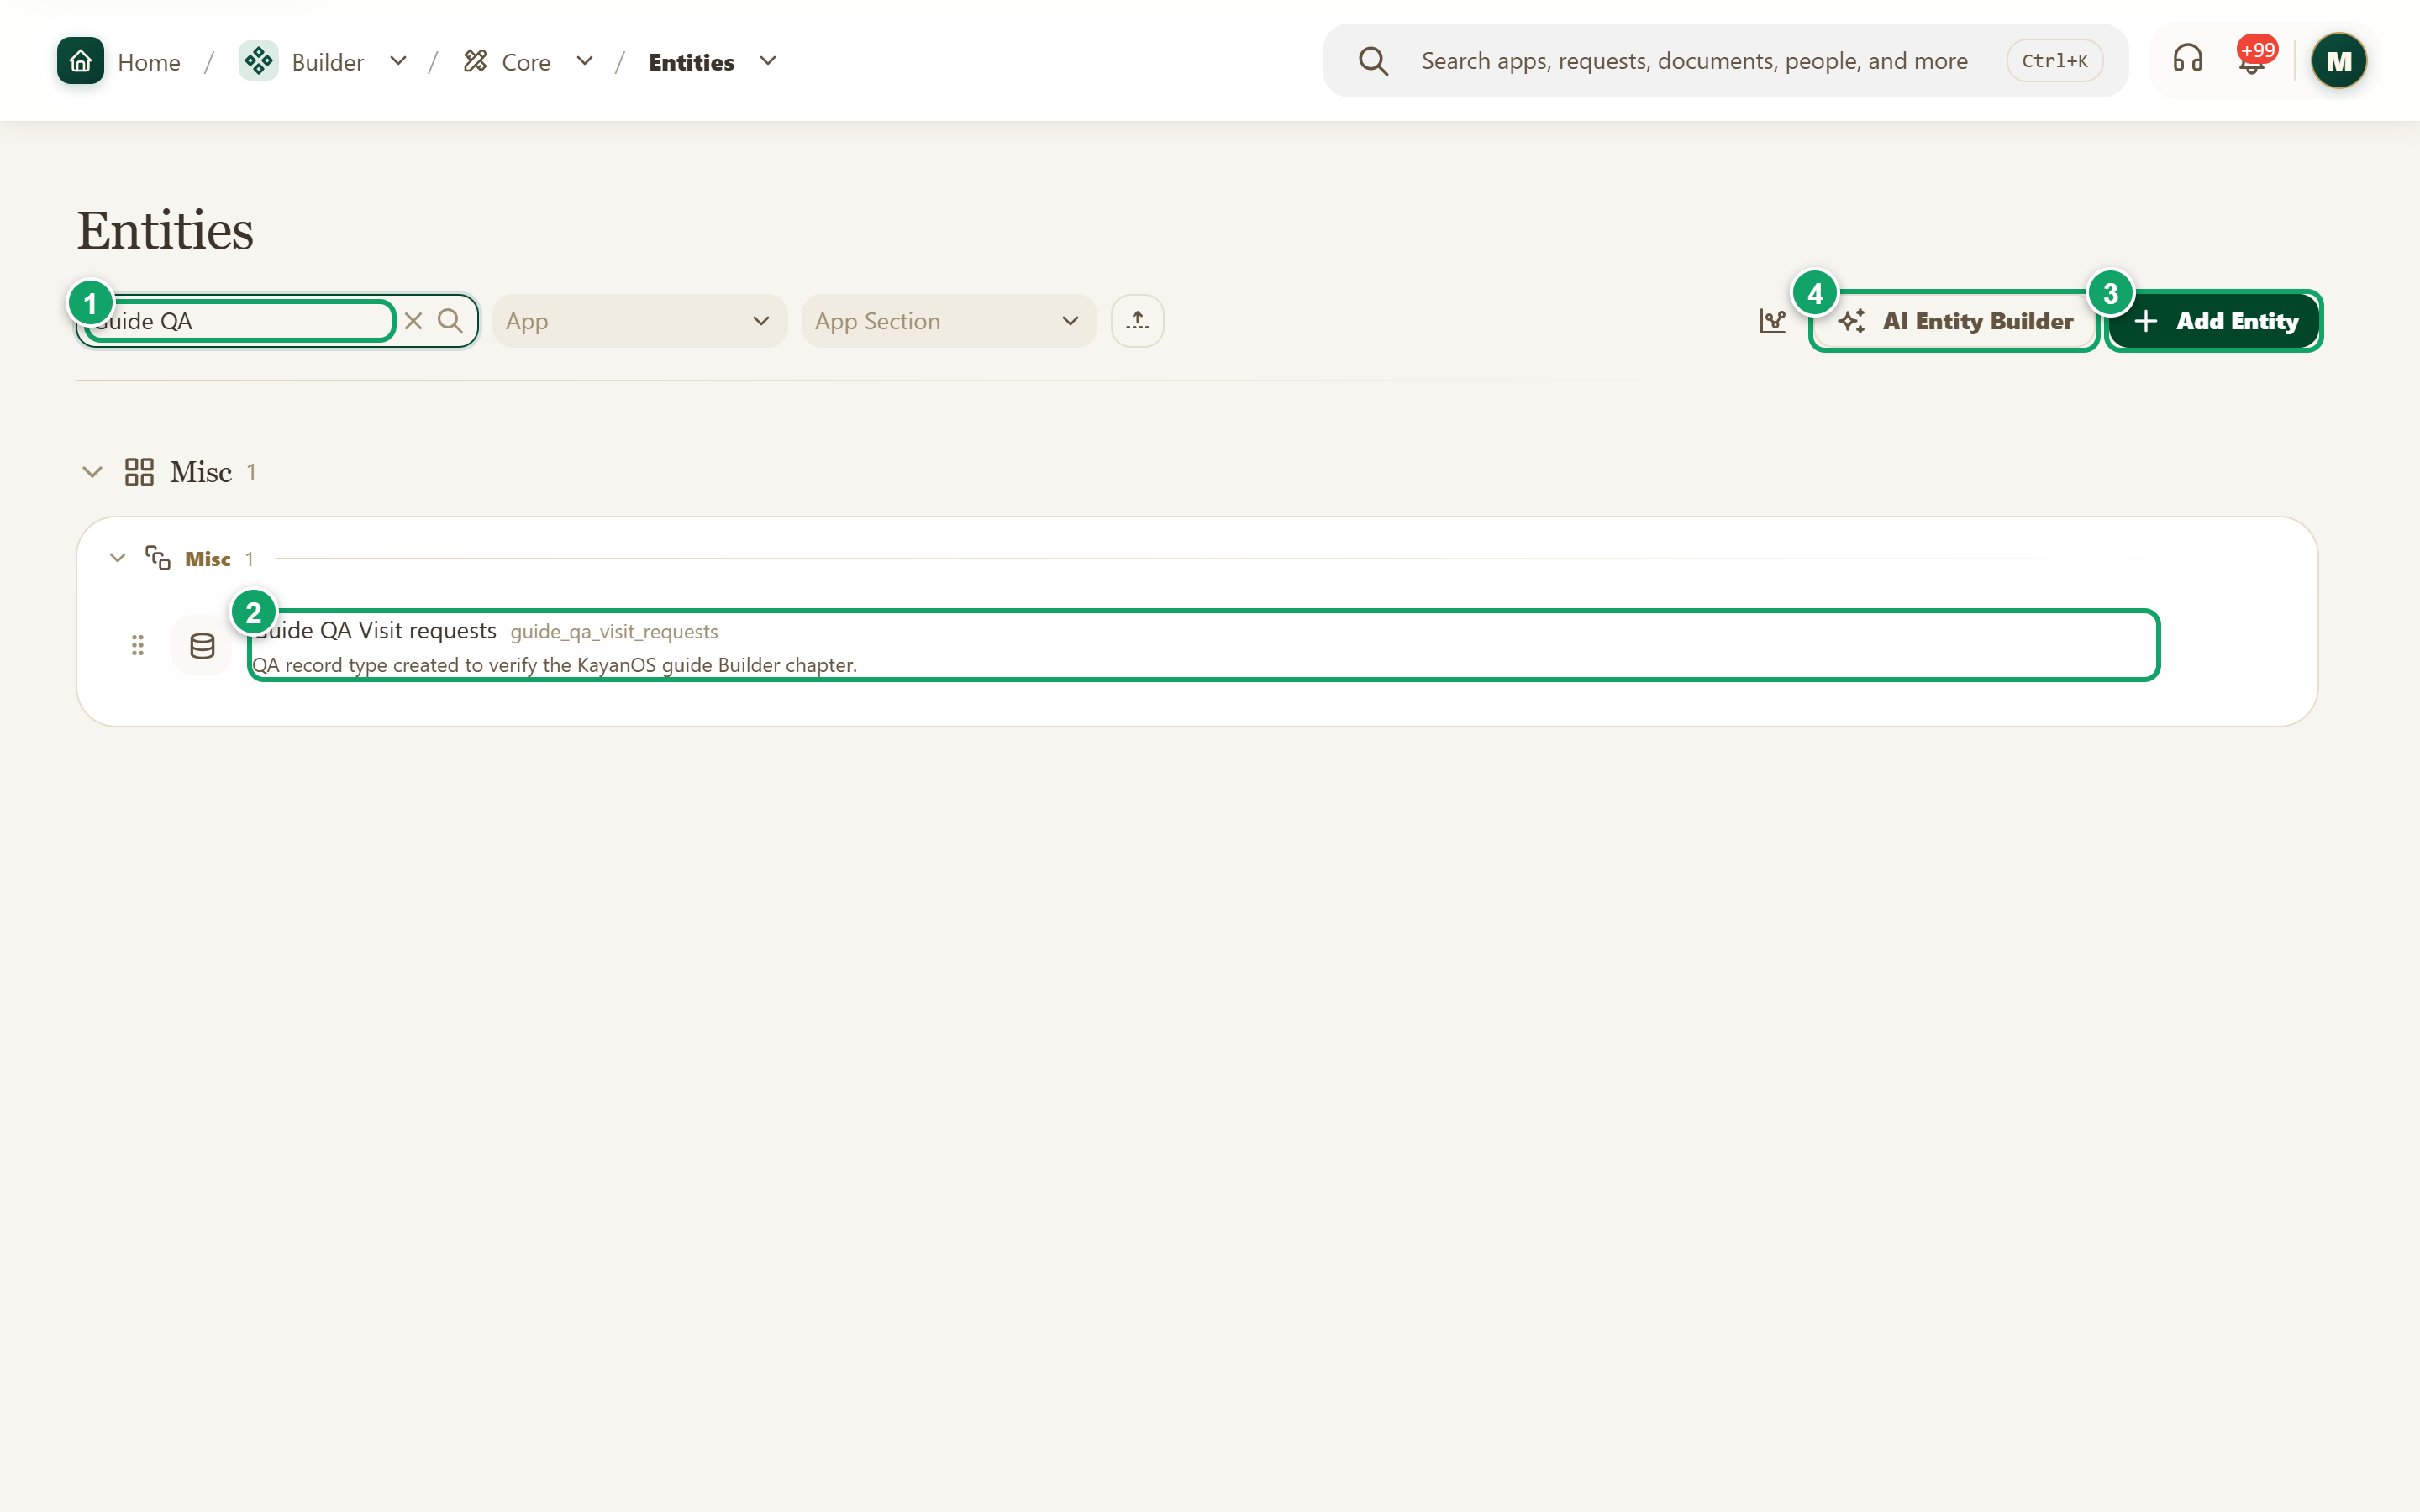
\includegraphics[width=0.95\linewidth,height=0.72\textheight,keepaspectratio]{figures/screens/ch06-entities-en.png}
\caption{The “Entities” page after searching for a record type}
\label{fig:builder-entities-screen}
\shotnote{The page lists record types grouped by app; here search narrowed it to one test record type created on test2 to verify this chapter. ① The search box: type part of the type’s name before creating a new one. ② The type you found: press it to open it in the “Builder” workspace. ③ “Add Entity”: creates a new type when you find nothing suitable. ④ “AI Entity Builder”: proposes fields from a description you write.}
\end{figure}


\begin{table}[H]
\centering
\caption{What do you find here?}
\label{tab:builder-entities-data}
\begin{tabularx}{\linewidth}{R{3.6cm} Y}
\rcHeaderRow
\thh{Section} & \thh{Content and action}\\
List of types & Record types grouped by app and section, each with its name, key and description. Narrow the list with search or the “App” and “App Section” filters.\\
Add Entity & Opens a page where you write the type's title, description and first fields, then press “Create Entity”.\\
AI Entity Builder & Describe the type you need in your own words and the system proposes its fields for you to review before saving. The button appears only when the organization has enabled AI in Builder.\\
View ERD Diagram & Draws the record types and the relationships between them, so you know what a type is linked to before you change it.\\
Open an existing type & Pressing a type opens it in the “Builder” workspace, where you edit its fields, page and lists and publish the changes.\\
\end{tabularx}
\end{table}

\begin{figure}[H]
\centering
\begin{tikzpicture}[node distance=0.5cm]
\node[stepBox] (a) {Look for a similar type};
\node[stepBox,below=of a] (b) {Add Entity, write its title};
\node[stepBox,below=of b] (c) {Create Entity};
\node[stepBox,below=of c] (d) {Open it in Builder};
\draw[flowsTo] (a) -- (b);
\draw[flowsTo] (b) -- (c);
\draw[flowsTo] (c) -- (d);
\end{tikzpicture}
\rclegend
\caption{Creating a record type}
\label{fig:builder-entities-flow}
\shotnote{The diagram starts with a search because the type you need may already exist in a ready-made app, and a second copy splits the data between two places. After “Create Entity” you return to the entity list and open the new type in the “Builder” workspace to finish it; creating the type does not mean the application is ready for the team.}
\end{figure}

\subsection{Steps and check}
\begin{enumerate}
\item Open “Entities”, type a name close to what you need into search, and review the results before creating a new type.
\item Press “Add Entity”, write a plural title that describes the records, such as “Maintenance requests”, and add a short description.
\item Name the suggested first field or change its type, and press “Add New Field” for each other essential piece of information.
\item Press the settings button next to “Create Entity” to choose the app and section where the type appears, then press “Create Entity”.
\end{enumerate}

\textbf{Check and recovery:} a success message should appear and the new type should show in the “Entities” list under the app you chose. If “Create Entity” stays disabled, write the type's title first; if you cannot find the type in the list, clear the app and section filters and search by its name.

\clearpage
\section{AI Entity Builder and relationship diagram}
\label{sec:builder-feature-ai-builder}

Instead of adding fields one by one, you can describe the record type you need in your own words: the “AI Entity Builder” proposes its fields, tabs and sections, and you review and edit the proposal before saving it. This helps when the type is large or when you want a quick starting point. “View ERD Diagram” draws the existing record types and the relationships between them, so before any change you know what is linked to the type you are about to edit.

\textbf{Path and who uses it:} “Entities” → “AI Entity Builder”, or the “View ERD Diagram” button in the header of the same page. The AI button shows when “AI in builders” is on in the organization's settings, and saving needs permissions to create and update entities and to create fields.

\begin{rcnote}[Example: Horizon]
Horizon's system administrator writes: “Create a record type for branch visit requests, with the branch, the visit date, its purpose and the requester.” They answer two questions the assistant asks, review the proposed fields, and press “Validate” before “Save Entity”.
\end{rcnote}

\begin{figure}[H]
\centering
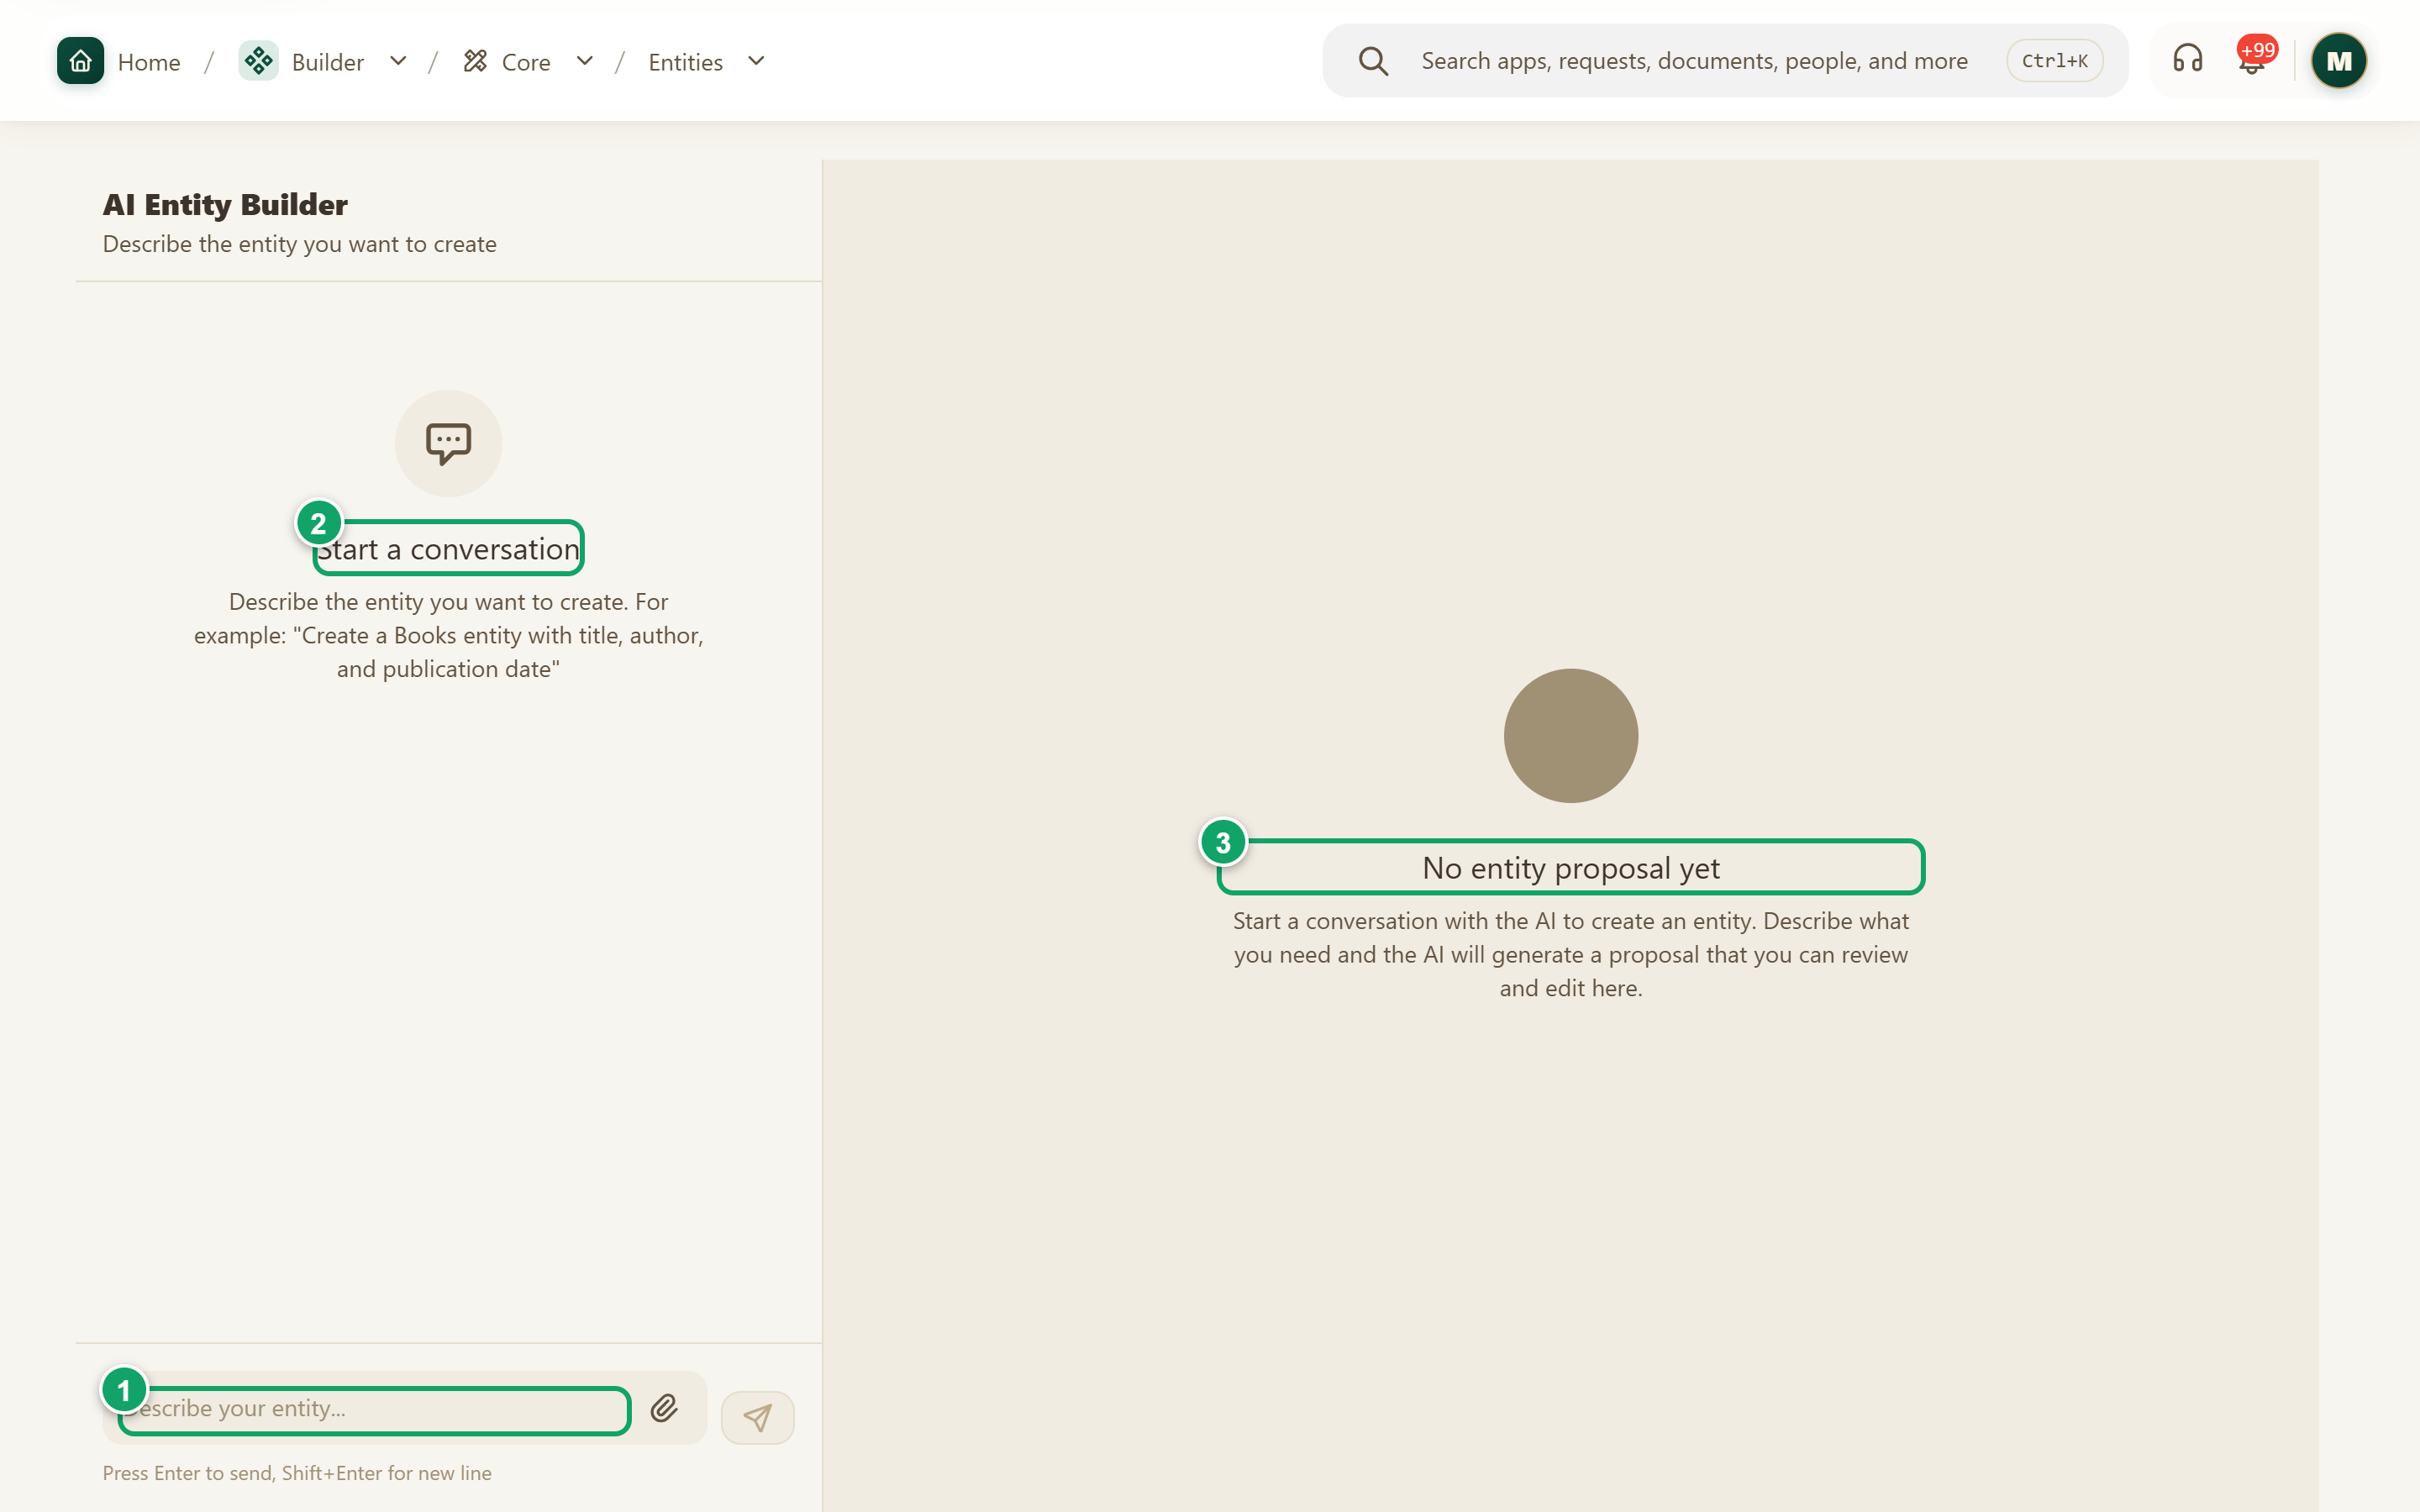
\includegraphics[width=0.95\linewidth,height=0.72\textheight,keepaspectratio]{figures/screens/ch06-ai-builder-en.png}
\caption{The AI Entity Builder before the conversation starts}
\label{fig:builder-ai-builder-screen}
\shotnote{The screen shows the assistant before any conversation: the chat on one side and the proposal preview on the other, empty until the assistant proposes a type. It shows where you write and where you review the result before saving. ① The “Describe your entity...” box: write the type description here. ② “Start a conversation”: an example of a suitable description to follow. ③ “No entity proposal yet”: the place of the “Entity Preview”, which fills after the first proposal.}
\end{figure}

\begin{table}[H]
\centering
\caption{What is in the AI Entity Builder?}
\label{tab:builder-ai-builder-parts}
\begin{tabularx}{\linewidth}{R{3.6cm} Y}
\rcHeaderRow
\thh{Part} & \thh{What it offers}\\
Chat & You describe the type in the “Describe your entity...” box, and you may attach a file that explains your work. The assistant may ask clarifying questions; you answer them and press “Submit Answers”.\\
Entity Preview & Shows the whole proposal: key, title and description, tabs and sections, custom actions, and the fields table. You can edit any part before saving.\\
Validate & Checks the proposal and lists what it finds under “Validation Issues”, with a suggestion for each. Errors block saving; warnings do not.\\
Ask AI to Fix & Sends the issues to the chat, so the assistant corrects its proposal instead of you editing it by hand.\\
Save Entity & Creates the type and its fields after “Confirm Save”. The button works only after a successful validation without errors, made after your last edit.\\
Download JSON & Saves the proposal as a file to keep or to share with a colleague for review.\\
Relationship diagram & Shows each type with its fields and draws relationships as arrows labelled with the linking field. Clicking a type highlights its links, and “Download Structure” saves a text description of all types and their relationships.\\
\end{tabularx}
\end{table}

\begin{rcwarn}[Saving here skips the draft]
Unlike the Builder workspace, the type and its fields are created directly after “Confirm Save”, and you return to the “Entities” list. So review the proposal carefully before saving, then open the type in the Builder workspace to complete its page, rules and access. When the proposal modifies an existing type, saving only adds new fields and leaves existing ones unchanged.
\end{rcwarn}

\begin{figure}[H]
\centering
\begin{tikzpicture}[node distance=0.5cm]
\node[stepBox] (a) {Describe the type in chat};
\node[stepBox,below=of a] (b) {Answer the questions};
\node[stepBox,below=of b] (c) {Review the Entity Preview};
\node[stepBox,below=of c] (d) {Validate};
\node[stepBox,below=of d] (e) {Save Entity};
\node[stepBox,below=of e] (f) {Complete it in the workspace};
\draw[flowsTo] (a) -- (b);
\draw[flowsTo] (b) -- (c);
\draw[flowsTo] (c) -- (d);
\draw[flowsTo] (d) -- (e);
\draw[flowsTo] (e) -- (f);
\end{tikzpicture}
\rclegend
\caption{Creating a record type with AI assistance}
\label{fig:builder-ai-builder-flow}
\shotnote{The diagram places “Validate” before saving because the button does not work without it, and every edit in the preview needs a new validation. The last step reminds you that the assistant only proposes fields and tabs; the record page, rules and access are set afterwards in the Builder workspace.}
\end{figure}

\subsection{Steps and check}
\begin{enumerate}
\item Open “Entities” and press “View ERD Diagram”, then look for a type close to what you need so you do not duplicate an existing one.
\item Press “AI Entity Builder”, write a description of what one record represents and the information it keeps, then press \en{Enter}.
\item Answer the clarifying questions if they appear, and press “Submit Answers”.
\item Review the “Entity Preview”: the type's name and key, the field types and the tabs. Edit what is needed directly or ask for the change in the chat.
\item Press “Validate”, fix errors yourself or with “Ask AI to Fix”, then press “Save Entity” and “Confirm Save”.
\end{enumerate}

\textbf{Check and recovery:} the message “Entity saved successfully” should appear and the type should show in the “Entities” list. If “Save Entity” stays disabled, press “Validate” again after your last edit, or hover over it to see missing permissions. If the AI button does not appear at all, ask the organization's administrator to turn on “AI in builders”.

\clearpage
\section{The Builder workspace and Overview}
\label{sec:builder-feature-workspace}

The Builder workspace is where you edit a record type after creating it; you open it by pressing the type on the “Entities” page. Its sections appear in a side menu in this order: “Overview”, “Fields”, “Record page”, “Lists \& views”, “Rules”, “Access”, “Movement”, “Evidence”, “Actions \& automations”, “Import” and “Advanced”. The “Overview” section summarizes the whole type in one place and tells you what must be fixed before publishing.

\textbf{Path and who uses it:} “Entities” → press the record type → “Overview”. The person who builds the type uses it every time they return, to know what changed and what is still missing.

\begin{rcnote}[Example: Horizon]
The administrator opens “Visit requests” and sees in “Overview” that three fields are not on any page yet, and that “Before you publish” shows a warning for a label with no English text. They place the fields on the page and translate the label, then press “Review \& publish”.
\end{rcnote}

\begin{figure}[H]
\centering
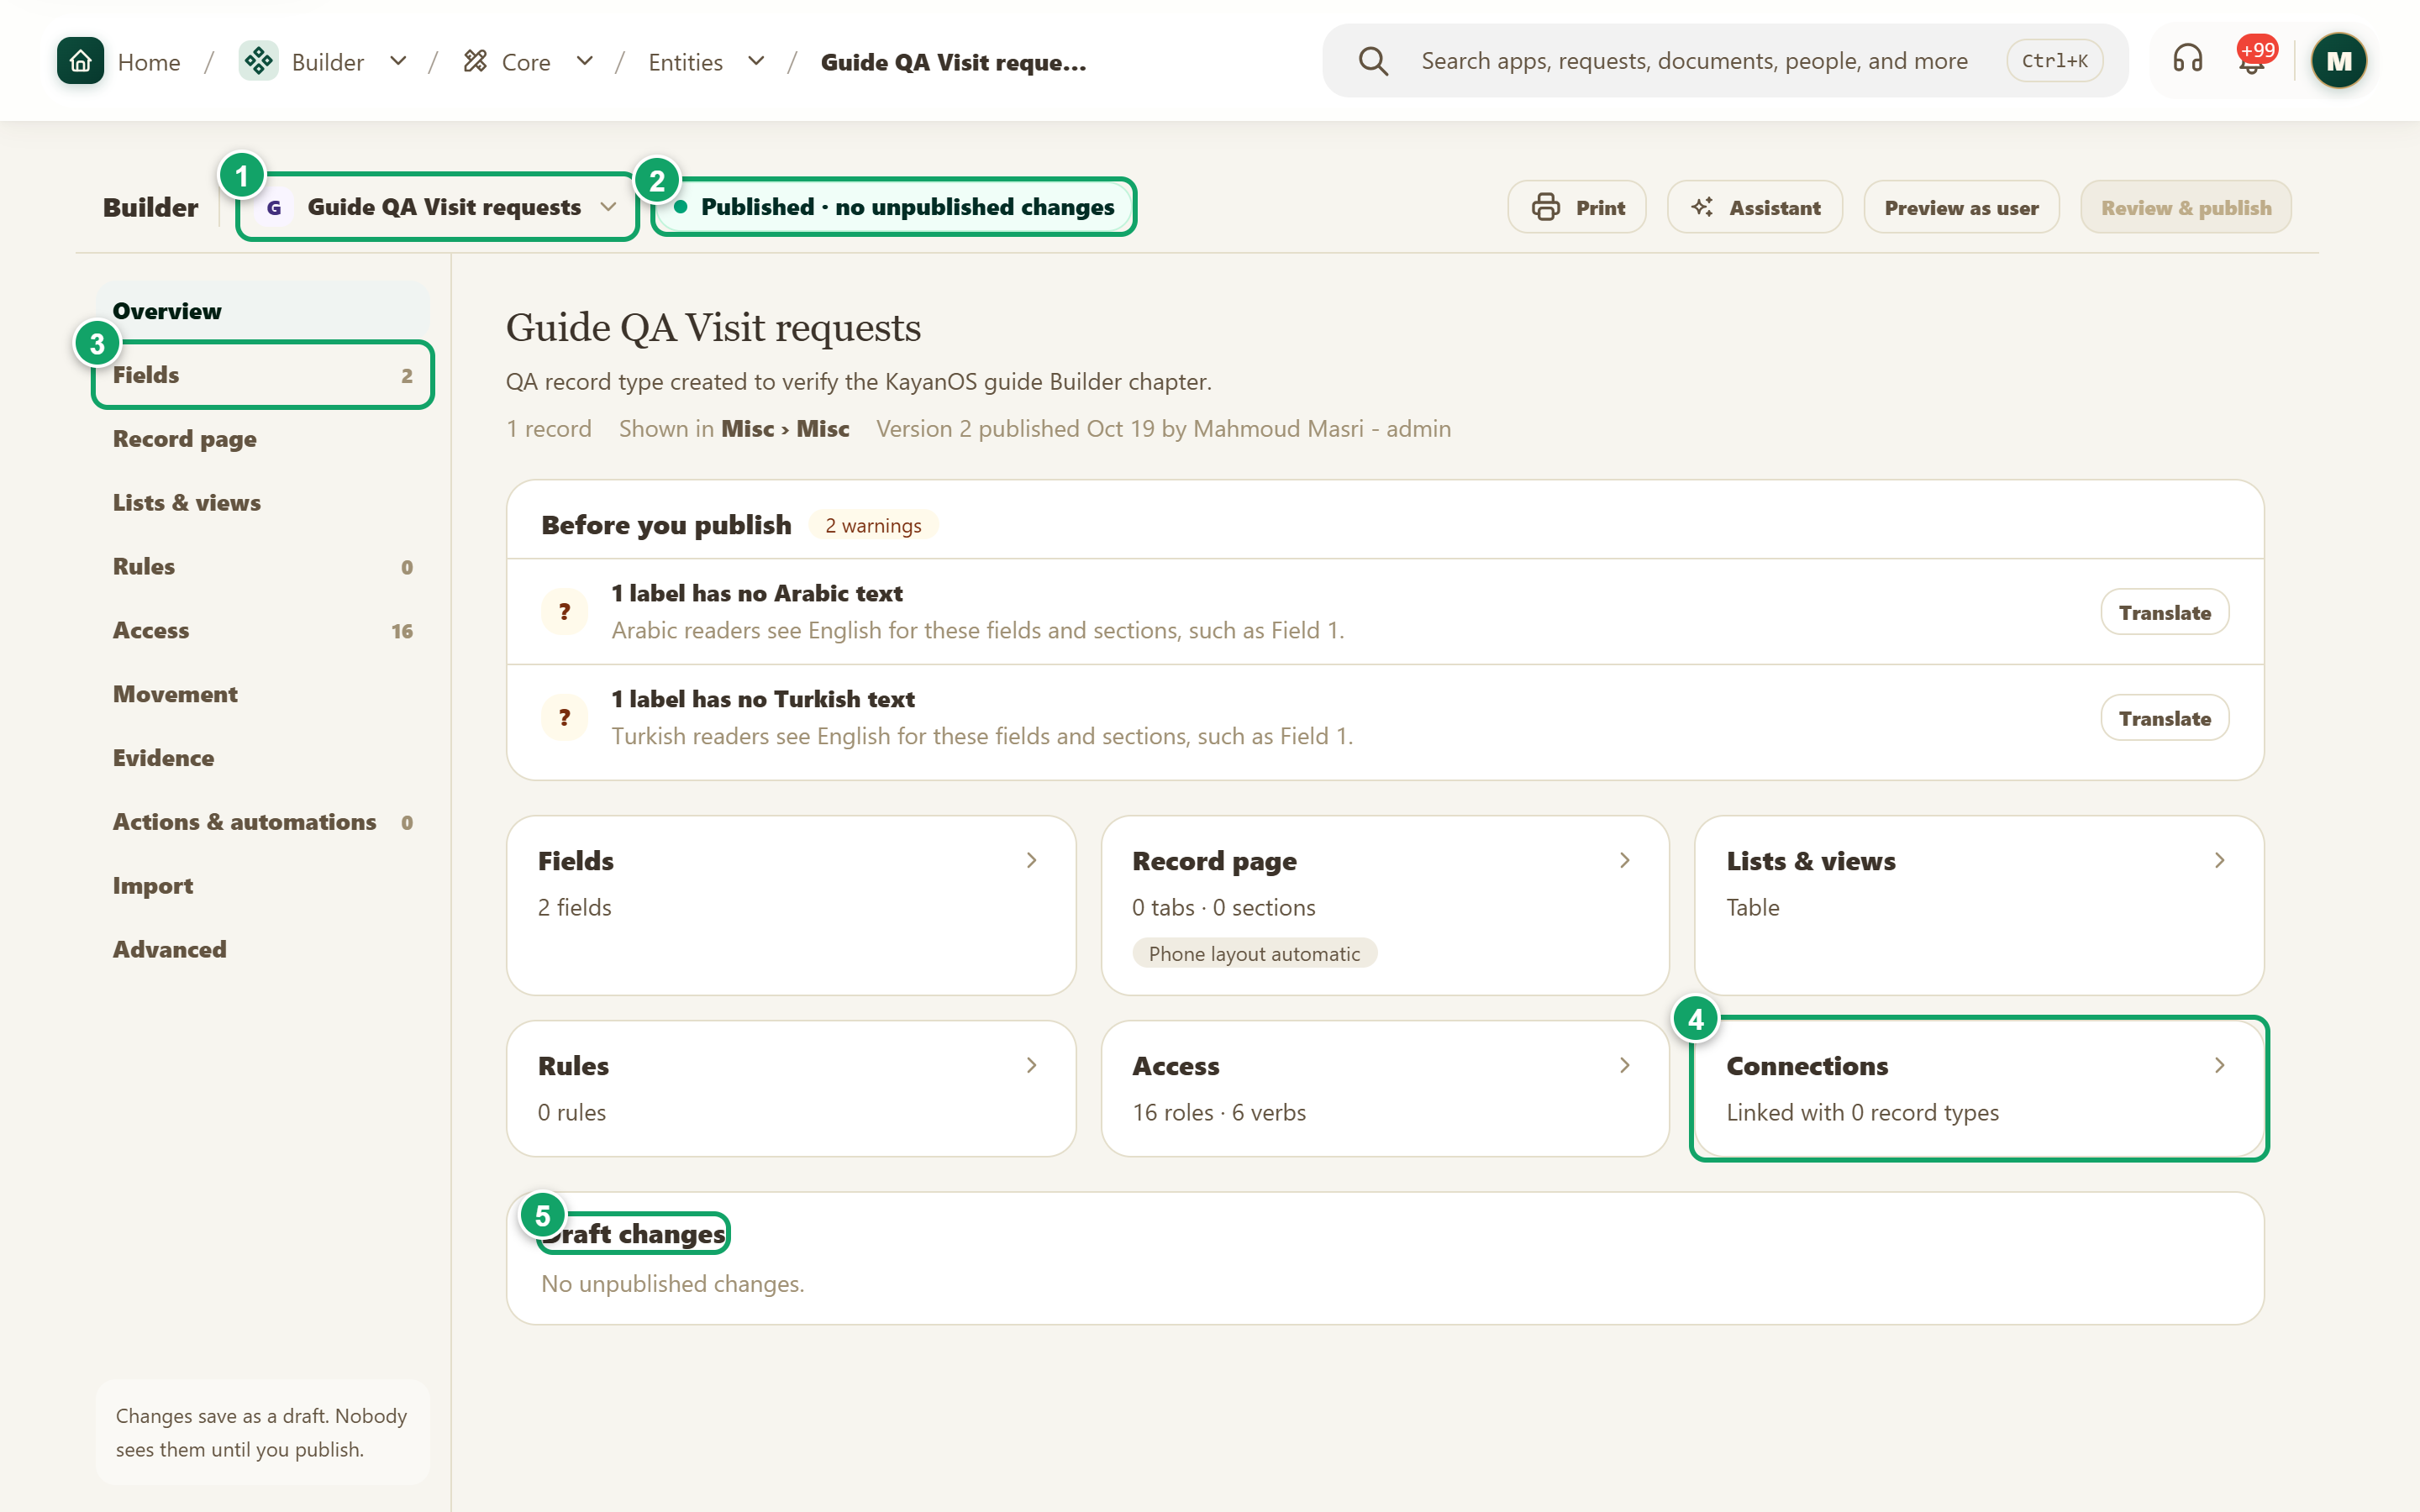
\includegraphics[width=0.95\linewidth,height=0.72\textheight,keepaspectratio]{figures/screens/ch06-ws-header-en.png}
\caption{The workspace header and the “Overview” section of a test record type}
\label{fig:builder-workspace-screen}
\shotnote{The image shows the test record type created on test2 to verify this guide, open in the Builder workspace on “Overview”. The header, side menu and cards gather what you need to know before any change. ① The record-type switcher. ② The status pill: says the type is published with no pending changes. ③ “Fields” in the side menu: the number next to it is the field count. ④ The “Connections” card. ⑤ “Draft changes”: what is not published yet.}
\end{figure}

\begin{table}[H]
\centering
\caption{The workspace header}
\label{tab:builder-workspace-header}
\begin{tabularx}{\linewidth}{R{3.6cm} Y}
\rcHeaderRow
\thh{Item} & \thh{What it offers}\\
Record-type switcher & Moves you to another type without returning to the list, with a “Find a record type” search.\\
Status pill & Says “Published · no unpublished changes” when the type matches what the team sees, or “Draft” with the number of unpublished changes and the time of the last save.\\
Print & Opens the record type's print templates; their number shows on the button when there are any.\\
Assistant & Opens the “Builder assistant”: you ask it for a field, a rule or a formula, it proposes changes to the draft, and you apply the ones you want. Nothing is published until you review and publish.\\
Preview as user & Shows the record page as a given role or person sees it, without saving anything.\\
Review \& publish · N & Opens the review dialog; the number is the count of changes in the draft. The button is disabled when there are no changes.\\
\end{tabularx}
\end{table}

\begin{table}[H]
\centering
\caption{The parts of “Overview”}
\label{tab:builder-workspace-cards}
\begin{tabularx}{\linewidth}{R{3.6cm} Y}
\rcHeaderRow
\thh{Part} & \thh{What it tells you}\\
Page header & The type's name and description, the number of records, the app and section under “Shown in”, and the published version and who published it. “Open list” opens the list of records.\\
Fields & The number of fields, how many are calculated or rolled up, and the fields not placed on any page.\\
Record page & The number of tabs and sections, and whether overview blocks are on.\\
Lists \& views & The available views and the default one, and the number of figures and saved views.\\
Rules & The number of rules by kind, such as show or hide, editing and required.\\
Access & The number of roles, verbs and custom verbs, and the fields with their own access.\\
Connections & The number of record types linked with this type, so you know what an edit may affect.\\
Draft changes & The unpublished changes since the draft started; “Review all” opens the review.\\
Before you publish & The problems that block publishing and the warnings, each with a button that opens the place to fix it.\\
\end{tabularx}
\end{table}

\subsection{The “Before you publish” list}

This list checks the draft whenever you edit it. Some problems block publishing because records would not work with them, such as a rule or formula that points to a deleted field, an expression with a mistake, empty or duplicate choices, or deleting the field that holds the record's name. Warnings do not block publishing but deserve a look, such as a tab that is always empty, a field placed in a tab that does not exist, or labels without a translation. When the list is clear it shows “Nothing to fix. The draft can be published.”.

\begin{rcwarn}[When two people edit the same draft]
If someone else saves the draft after you opened it, “Someone else changed this draft” appears and your edits are not saved until you choose. Press “Reload their draft” to see their version and lose your unsaved edits, or “Overwrite with mine” to save your version over theirs. While testing this guide the message appeared for an older copy of the same session, so if you are sure nobody else is editing the type with you, choose “Overwrite with mine”.
\end{rcwarn}

\begin{figure}[H]
\centering
\begin{tikzpicture}[node distance=0.5cm]
\node[stepBox] (a) {Open the type from Entities};
\node[stepBox,below=of a] (b) {Read Overview};
\node[stepBox,below=of b] (c) {Edit in the sections};
\node[stepBox,below=of c] (d) {Fix Before you publish};
\node[stepBox,below=of d] (e) {Review and publish};
\draw[flowsTo] (a) -- (b);
\draw[flowsTo] (b) -- (c);
\draw[flowsTo] (c) -- (d);
\draw[flowsTo] (d) -- (e);
\end{tikzpicture}
\rclegend
\caption{A working session in the Builder workspace}
\label{fig:builder-workspace-flow}
\shotnote{The diagram starts by reading “Overview” because it shows the type's state before you change anything, and ends with publishing because edits stay in the draft until then. “Before you publish” comes right before the review, because a single problem blocks the whole publication until you fix it.}
\end{figure}

\subsection{Steps and check}
\begin{enumerate}
\item Open “Entities” and press the record type; the Builder workspace opens on “Overview”.
\item Read the status pill: if it says “Draft”, earlier changes have not been published, so review them in “Draft changes” before adding more.
\item Move to the section you want to edit from the side menu and make your changes; each edit is saved to the draft automatically.
\item Return to “Overview” and press the fix button next to each problem in “Before you publish” until no errors remain.
\end{enumerate}

\textbf{Check and recovery:} after each edit the status pill should change to “Draft” with the number of changes, and “Review \& publish” should become available. If “couldn't save, retrying on next change” appears, check your connection, then change any value so the save is retried.

\clearpage
\section{Fields}
\label{sec:builder-feature-fields}

A field defines one piece of information each record stores, such as a date, an amount or the person responsible. Choosing the right field type matters: it decides how the value is entered and checked, and allows sorting, filtering and calculation later. You add fields in the “Fields” section of the “Builder” workspace.

\textbf{Path and who uses it:} “Entities” → open the record type → “Fields”. Used by whoever builds the record type, before arranging its page and lists.

\begin{rcnote}[Example: Horizon]
The system administrator adds a “Serial ID” field to “Visit requests” that gives each request a number such as \en{HZN-VR-0001}, then a “Relation” field linking the request to the branch, a “Date” field for the visit date and a “Long Text” field for its purpose. Their steps match numbers ① and ③ on the image.
\end{rcnote}

\begin{figure}[H]
\centering
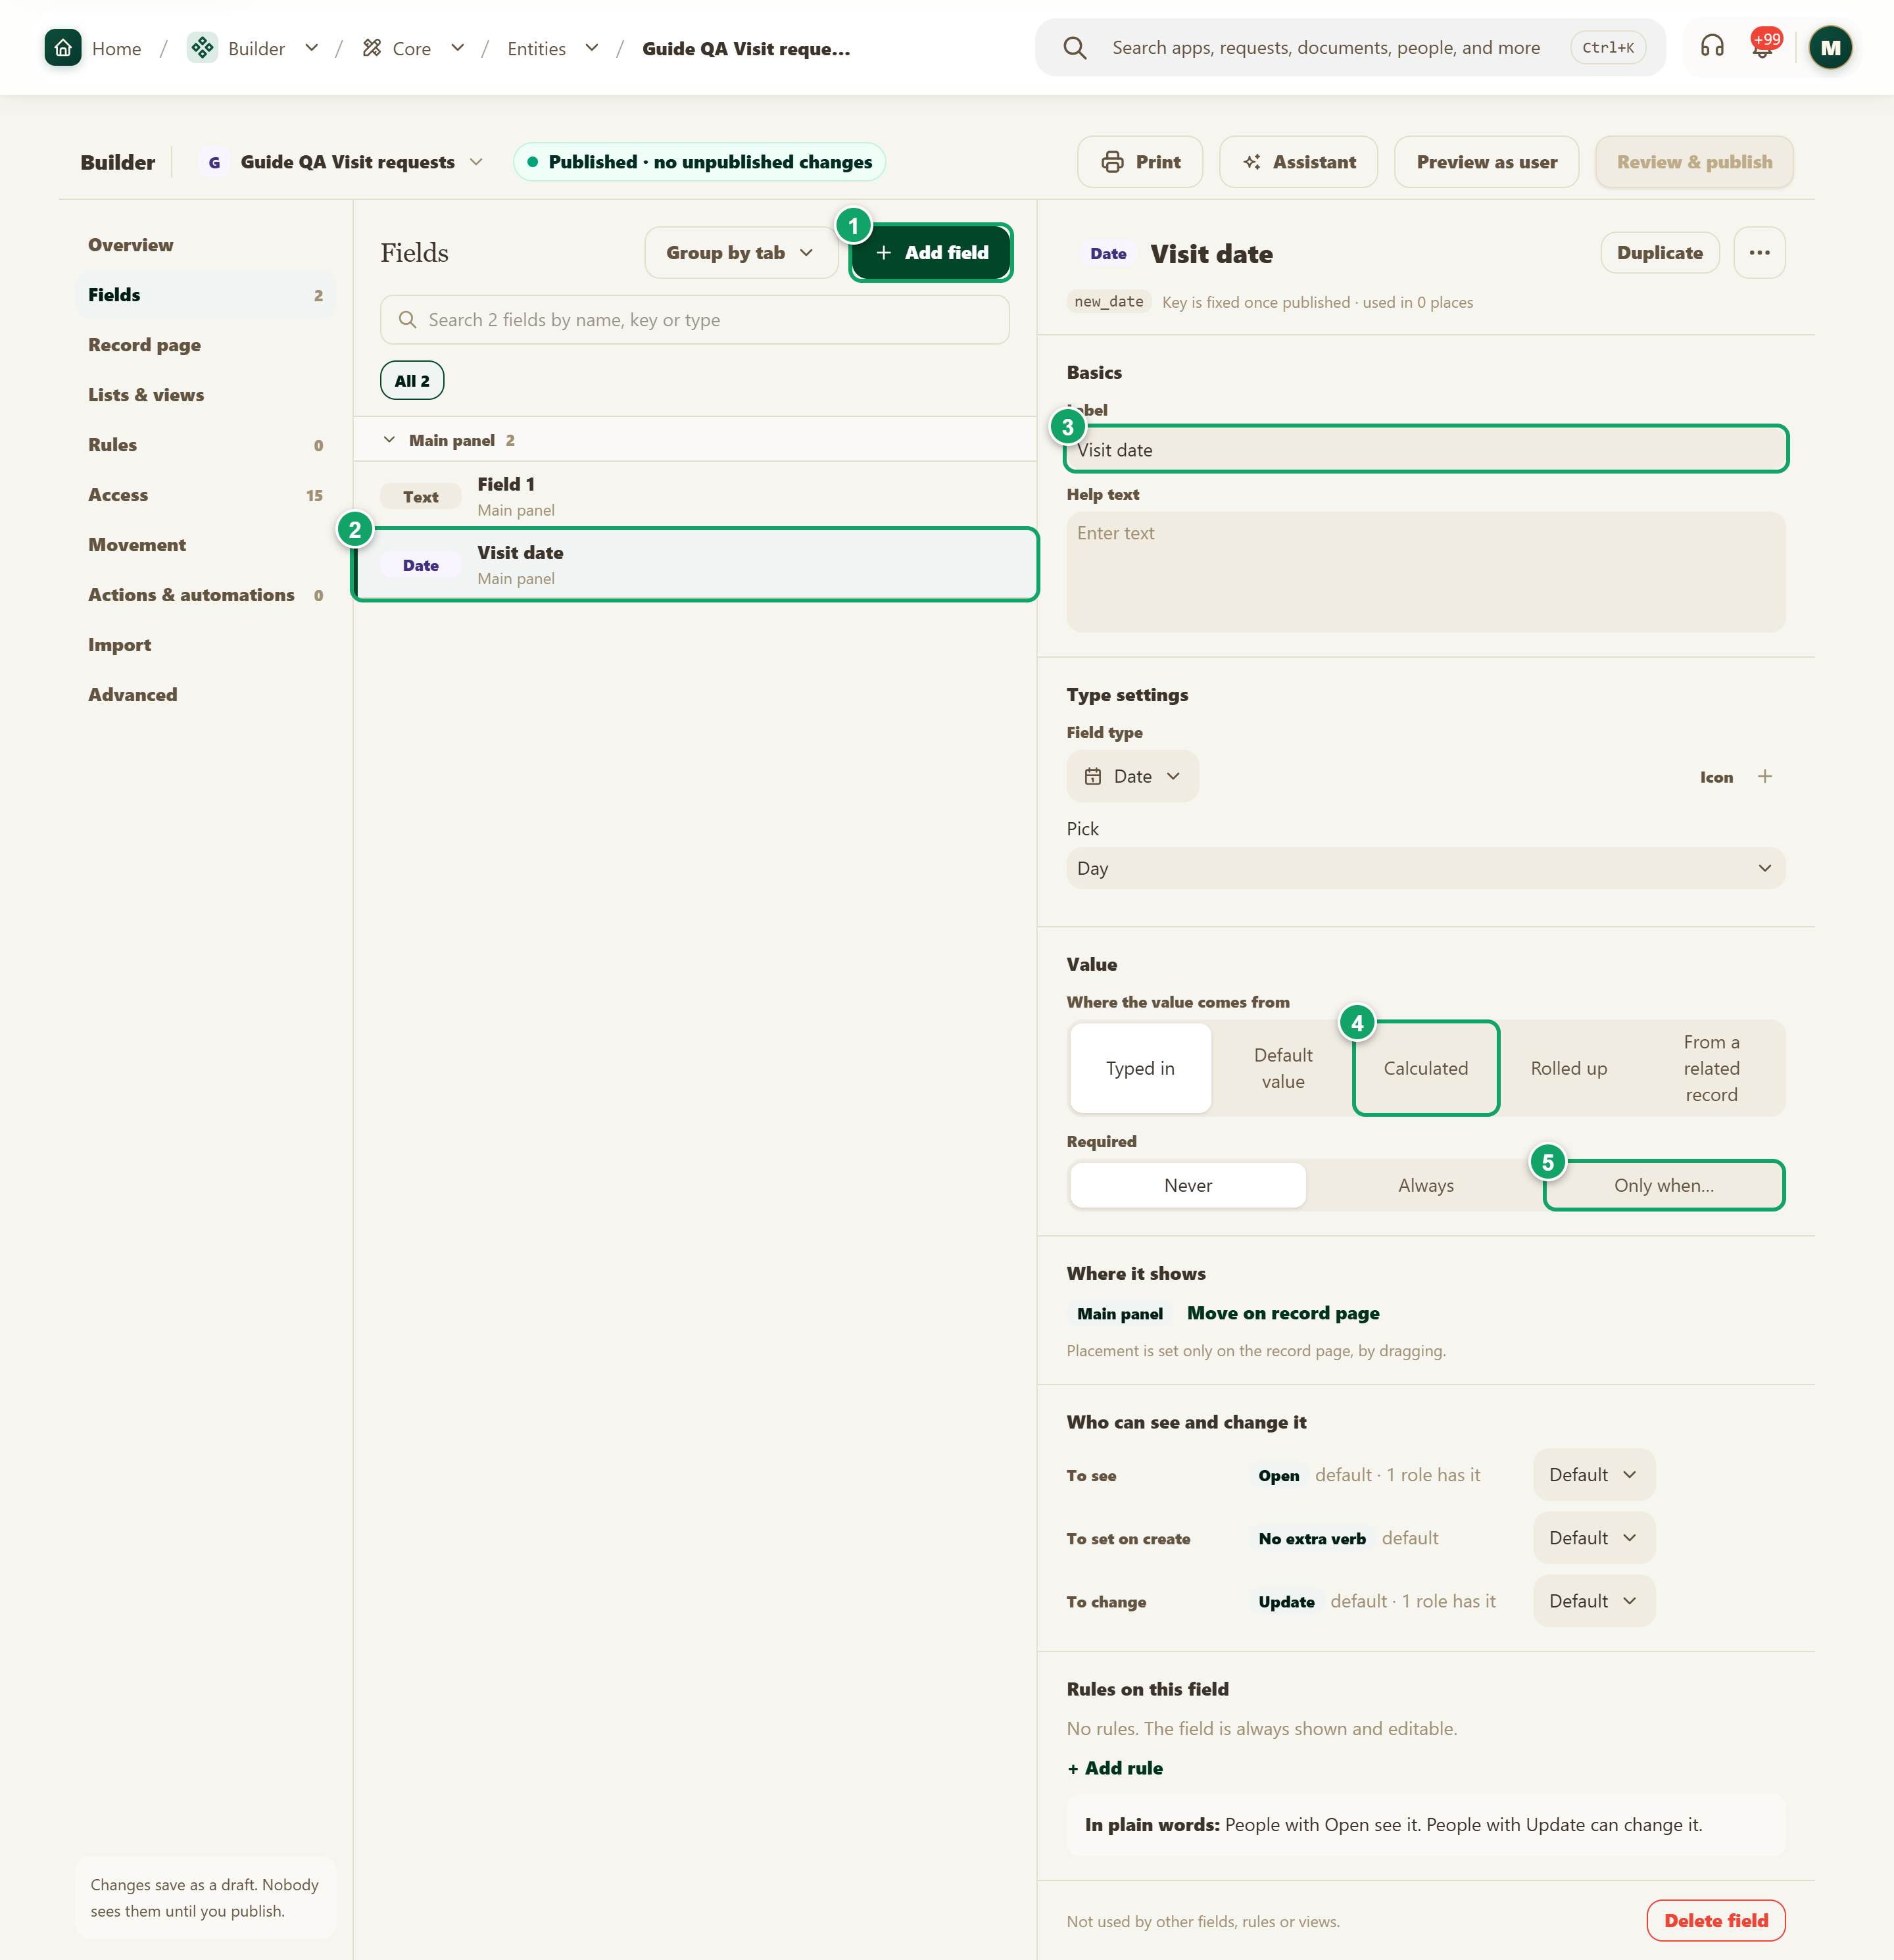
\includegraphics[width=0.95\linewidth,height=0.72\textheight,keepaspectratio]{figures/screens/ch06-ws-fields-en.png}
\caption{The “Fields” section and the settings of a date field}
\label{fig:builder-fields-screen}
\shotnote{The section lists the record type’s fields, and choosing one shows its settings beside it. The selected field is a “Date” field added and published while testing this chapter on test2. ① “Add field”. ② The selected field in the list. ③ “Label”. ④ “Calculated”: makes the value the result of a formula instead of something users type. ⑤ “Only when…”: makes the field required in a given situation.}
\end{figure}


\begin{table}[H]
\centering
\caption{Field types}
\label{tab:builder-fields-types}
\begin{tabularx}{\linewidth}{R{3.6cm} Y}
\rcHeaderRow
\thh{Group} & \thh{Types and when to use them}\\
Text & “Text” for a short value, “Long Text” for a description, “Rich Text” for formatted text and “Phone” for a phone number.\\
Numbers and IDs & “Number” for quantities and amounts, “Duration” for time spent and “Serial ID” for a reference number the system generates for each record.\\
Dates and times & “Date”, “Date \& Time” and “Time”, plus ranges such as “Date Range” when the information has a start and an end.\\
Choice and status & “Select” for a fixed list of values, “Boolean” for a yes-or-no answer and “Status” for work stages based on a status template.\\
Files and images & “File” for attachments and “Avatar” for an image that represents the record.\\
Links and people & “Relation” to link the record to a record of another type, and “Member Selector” to pick a member of the organization.\\
Maps & “Location” for a point on the map and “Boundary” for a drawn area such as a plot or facility boundary.\\
Action & An advanced field that works with the “Actions \& automations” section.\\
Calculated, lookup and rolled up & Values the user does not type: “Calculated” uses a formula over the record's fields, a lookup shows a value from a related record, and “Rolled up” sums or counts the values of related records.\\
\end{tabularx}
\end{table}

\begin{table}[H]
\centering
\caption{What do you set on each field?}
\label{tab:builder-fields-settings}
\begin{tabularx}{\linewidth}{R{3.6cm} Y}
\rcHeaderRow
\thh{Setting} & \thh{Meaning}\\
Label & The name the user sees; it can be written in more than one language.\\
Key & A fixed name the system uses in formulas and templates. Choose a clear one from the start, because references depend on it.\\
Help text & A short sentence telling the user what to enter in the field.\\
Required & Prevents saving the record while the field is empty. Use it only for information the work cannot be completed without.\\
\end{tabularx}
\end{table}

\begin{figure}[H]
\centering
\begin{tikzpicture}[node distance=0.5cm]
\node[stepBox] (a) {Add field};
\node[stepBox,below=of a] (b) {Choose the field type};
\node[stepBox,below=of b] (c) {Label and key};
\node[stepBox,below=of c] (d) {Required and help text};
\draw[flowsTo] (a) -- (b);
\draw[flowsTo] (b) -- (c);
\draw[flowsTo] (c) -- (d);
\end{tikzpicture}
\rclegend
\caption{Adding a field}
\label{fig:builder-fields-flow}
\shotnote{The diagram puts the type before the label because the type decides which settings follow, such as the options of a “Select” field or the linked type of a “Relation” field. Each addition is saved to the draft at once, but users do not see the new field until you publish the changes.}
\end{figure}

\subsection{Steps and check}
\begin{enumerate}
\item Open the record type from “Entities”, then choose the “Fields” section.
\item Press “Add field” and choose the type that matches the information; a date, for example, belongs in a “Date” field, not in “Text”.
\item Write the label and review the key, add help text when needed, then decide whether the field is required.
\item For a field computed from others, choose “Calculated” and write the formula; for a value from a related record, choose “Lookup field” after adding a “Relation” field.
\end{enumerate}

\textbf{Check and recovery:} the field should appear in the field list, and “Overview” should show the field count together with fields not yet placed on any page. If you picked the wrong type, fix it before publishing and before entering real records, because changing a type after data builds up is harder.

\clearpage
\section{Field types and their settings}
\label{sec:builder-feature-field-types}

A field's type decides how the value is entered, how it is checked, and what can be done with it later: sorting, filtering and calculating. This page therefore explains every type available in “Add field”, then the extra settings that appear under “Type settings” for some of them. Choose the type before entering real data, because changing it after records accumulate is harder.

\textbf{Path and who uses it:} Builder workspace → “Fields” → “Add field”, then “Type settings” in the field's settings panel. Used by the person who builds the record type.

\begin{rcnote}[Example: Horizon]
For the request number, the system administrator chooses the “Serial ID” type in “Automatic” mode and gives it a format that starts with \en{HZN-VR-}, so the first request is numbered \en{HZN-VR-0001}. For the branch they choose a “Relation” field linked to the branches record type.
\end{rcnote}

\begin{figure}[H]
\centering
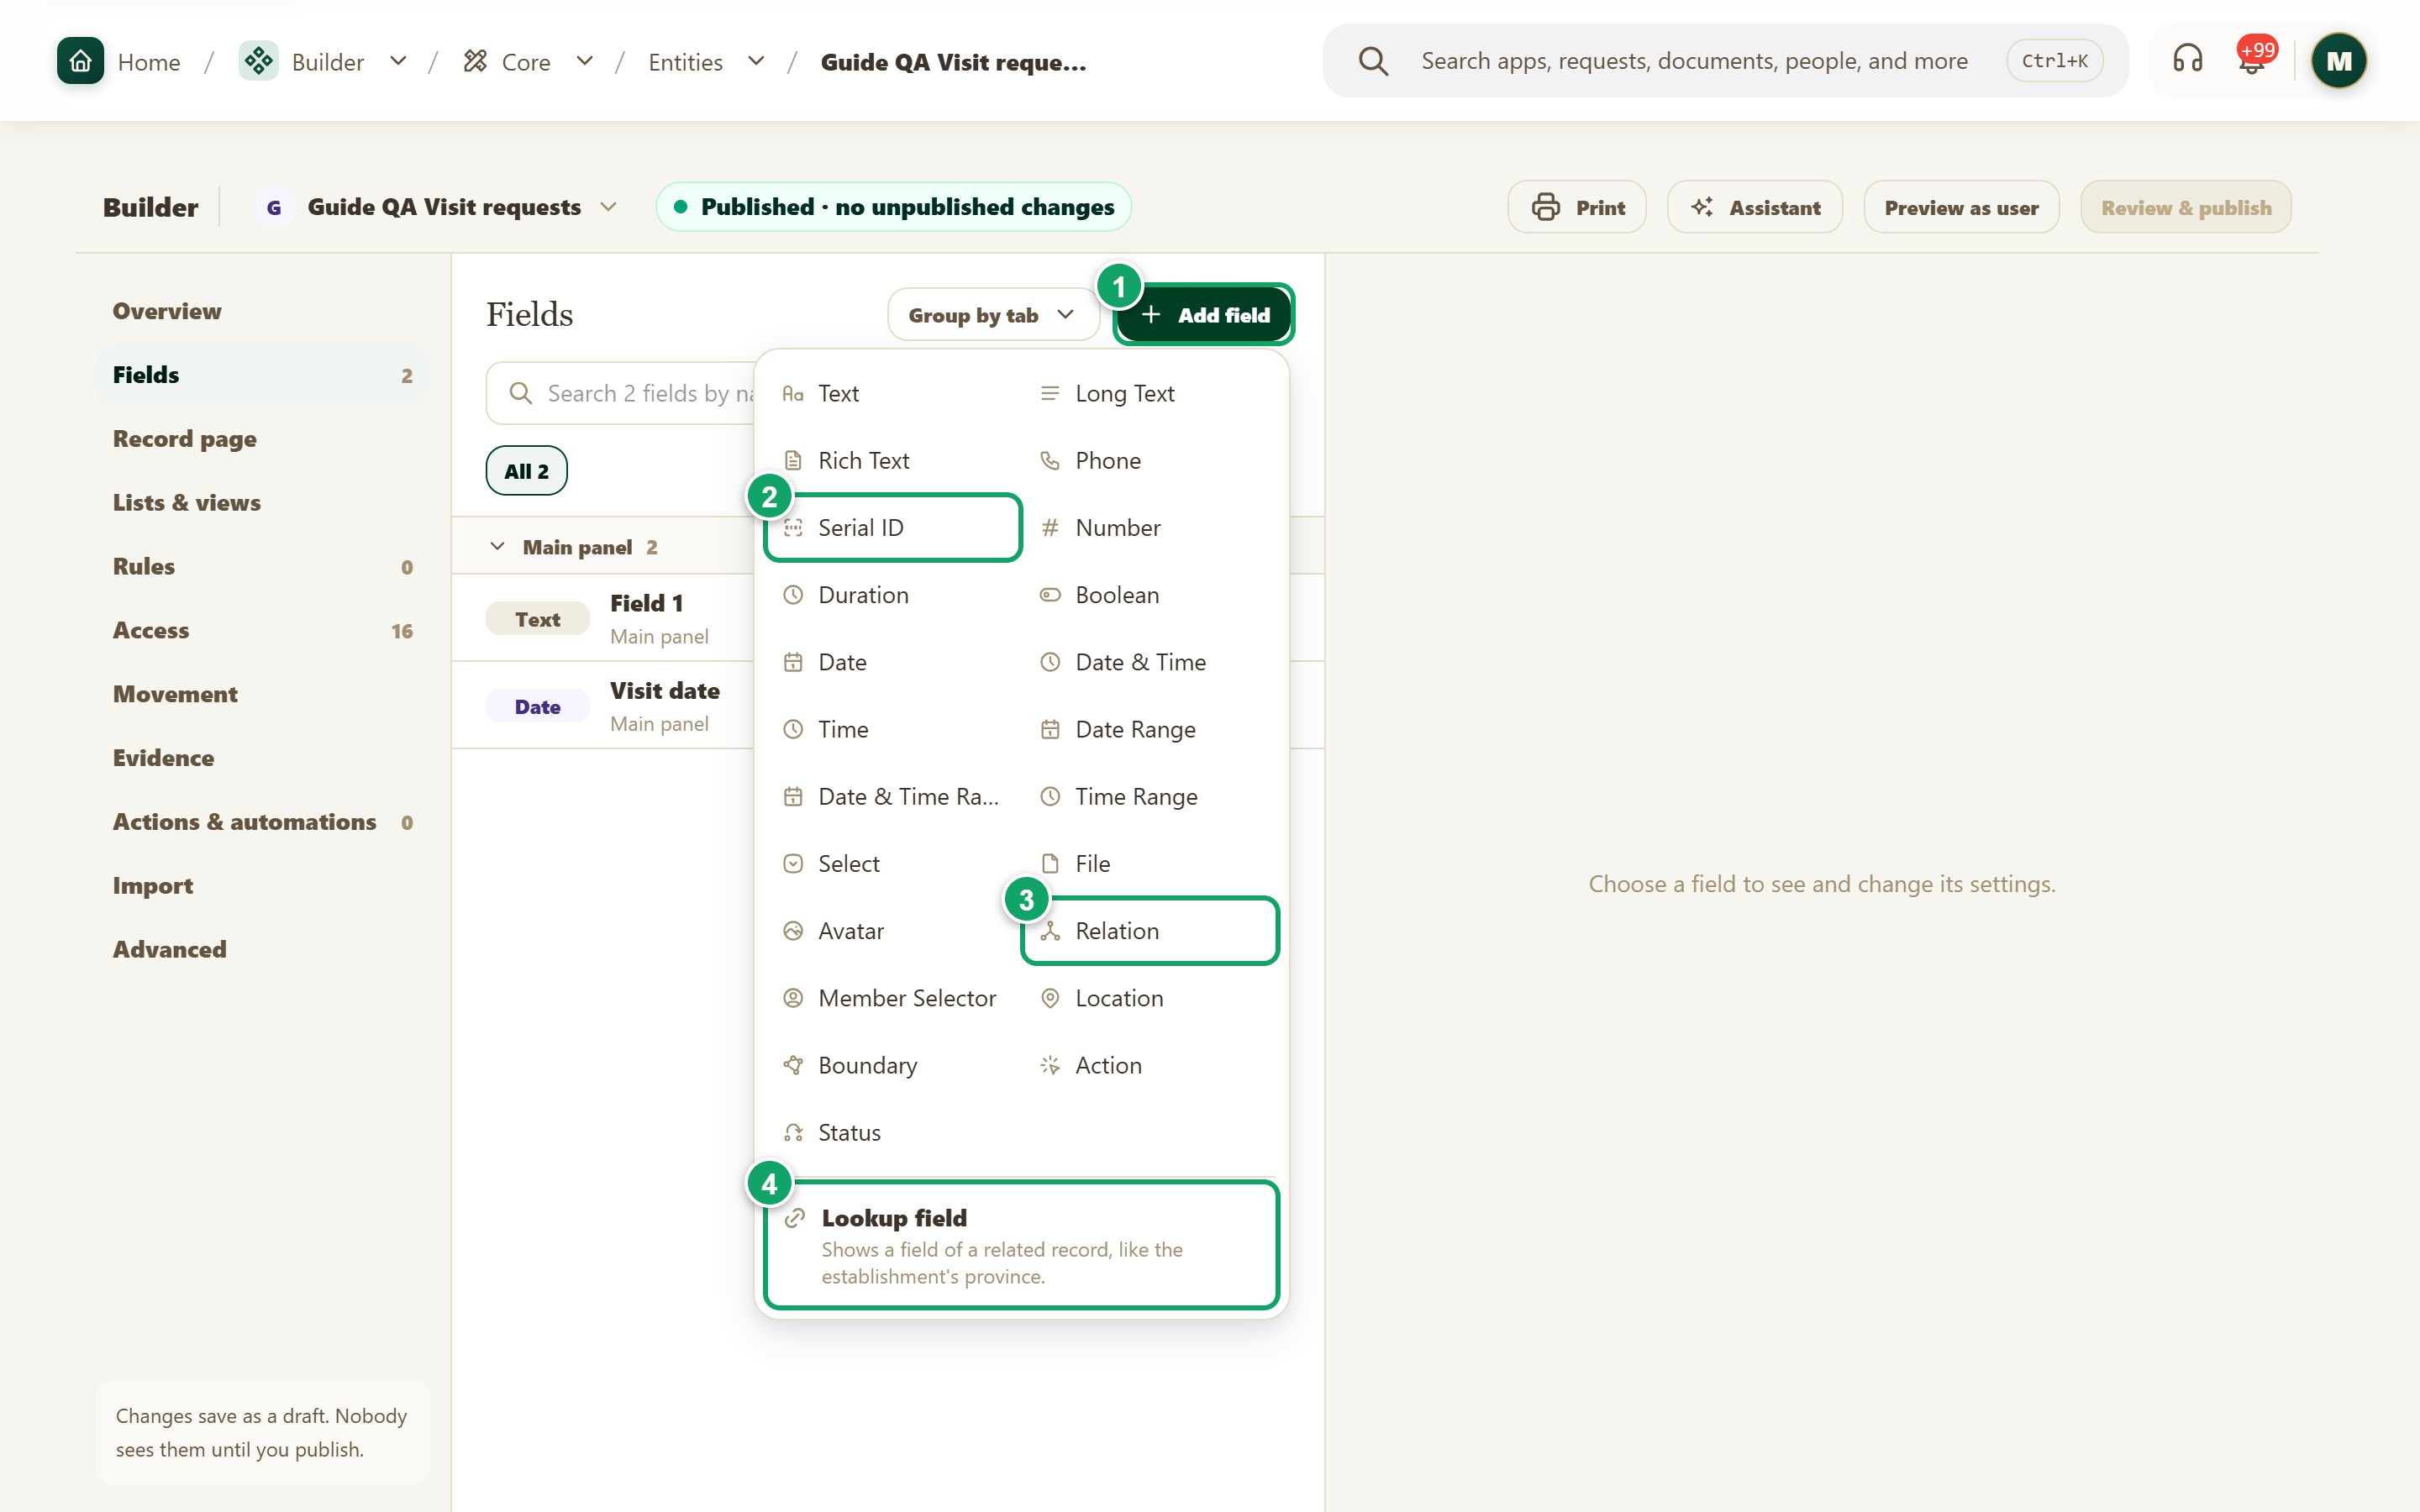
\includegraphics[width=0.95\linewidth,height=0.72\textheight,keepaspectratio]{figures/screens/ch06-ws-add-field-en.png}
\caption{The list of field types after pressing “Add field”}
\label{fig:builder-field-types-screen}
\shotnote{The image shows the list that opens when you add a field, with every available type in the order shown. It helps you choose the right type from the start instead of changing it after data is entered. ① “Add field”. ② “Serial ID”: a reference number the system generates. ③ “Relation”: links the record to a record of another type. ④ “Lookup field”: shows information from a related record.}
\end{figure}

\begin{table}[H]
\centering
\caption{Types available in “Add field”}
\label{tab:builder-field-types-all}
\begin{tabularx}{\linewidth}{R{3.6cm} Y}
\rcHeaderRow
\thh{Group} & \thh{Types and when to use each}\\
Text & “Text” for a short value such as a name, “Long Text” for a description or note, “Rich Text” for text with headings and lists, and “Phone” for a phone number.\\
Numbers and IDs & “Number” for quantities and amounts, “Duration” for time spent such as two hours, and “Serial ID” for a reference number the system generates for each record.\\
Yes or no & “Boolean” for a question answered yes or no, such as “Needs a car?”.\\
Dates and times & “Date”, “Date \& Time” and “Time” for a single value, and “Date Range”, “Date \& Time Range” and “Time Range” for information with a start and an end.\\
Choice and status & “Select” for a fixed list of values, and “Status” for work stages following a status template, such as “New”, then “Under review”, then “Approved”.\\
Links and people & “Relation” to link the record to a record of another type, “Member Selector” to pick a member of the organization, and “Lookup field” to show information from a related record without typing it again.\\
Files and images & “File” for attachments, and “Avatar” for an image that represents the record in lists and cards.\\
Maps & “Location” for a point on the map, and “Boundary” for an area drawn on the map with its area and perimeter, such as a plot or facility boundary.\\
Action & A button inside the record that creates a Word document or an Excel sheet, opens a link, or starts a workflow.\\
\end{tabularx}
\end{table}

\begin{table}[H]
\centering
\caption{Extra settings by type}
\label{tab:builder-field-types-settings}
\begin{tabularx}{\linewidth}{R{3.6cm} Y}
\rcHeaderRow
\thh{Type} & \thh{What you set in “Type settings”}\\
Select and Status & “Choices” and their colours, “Allow adding options” if users may add a new value, and a number for each option when you need calculations.\\
Relation & “Links to” to choose the other record type, and what happens to the record when the linked record is deleted: block the deletion, clear the field, or delete the dependent records with it. “Show relation in tab” and “Relations display” choose how these records appear on the other record's page, including a “Checklist” answered in place.\\
Serial ID & “Serial mode”: “Automatic”, “On request” or both, “Manual serial entry”, the “Format JEXL” that sets the number's shape, “Start at” and “Timezone”.\\
Status & The status template that defines the stages: a “Fixed template” for all records, or a “Per-record template” chosen from another field.\\
Member Selector & “Display As”: the member's details as fields inside the section, or as a separate tab on the record page.\\
File & File limits narrower than the organization's, such as the allowed file types.\\
Location and Boundary & The coordinate format: latitude and longitude, \en{MGRS} or \en{UTM}.\\
All types & “Allow several values” to keep more than one value in the same field, and “Text per language” for text written in Arabic and English.\\
\end{tabularx}
\end{table}

\begin{figure}[H]
\centering
\begin{tikzpicture}[node distance=0.5cm]
\node[stepBox] (a) {Add field};
\node[stepBox,below=of a] (b) {Choose the matching type};
\node[stepBox,below=of b] (c) {Type settings};
\node[stepBox,below=of c] (d) {One value or several};
\node[stepBox,below=of d] (e) {Try it in a record};
\draw[flowsTo] (a) -- (b);
\draw[flowsTo] (b) -- (c);
\draw[flowsTo] (c) -- (d);
\draw[flowsTo] (d) -- (e);
\end{tikzpicture}
\rclegend
\caption{Choosing and setting a field type}
\label{fig:builder-field-types-flow}
\shotnote{The diagram makes “Type settings” a step of its own because some types do not work without it: a “Relation” field needs the linked type, and a “Select” field needs its choices. The last step reminds you to try the field in a real record after publishing, because the input only shows fully there.}
\end{figure}

\subsection{Steps and check}
\begin{enumerate}
\item In “Fields” press “Add field”, and choose the type that matches the information, not its look; a phone number is “Phone”, not “Number”.
\item Open “Type settings” and complete what the type requires: the choices for “Select”, the linked type for “Relation”, and the format for “Serial ID”.
\item Turn on “Allow several values” only if one record really needs more than one value, such as several attachments.
\item Publish the changes, then create a test record and enter a value in the new field.
\end{enumerate}

\textbf{Check and recovery:} the field should accept the right value in the expected form, such as a date picker in a “Date” field. If “Before you publish” shows an error about empty or duplicate choices, open “Choices” and complete the values or delete the duplicate.

\clearpage
\section{Where the value comes from: calculated, lookup and rolled-up fields}
\label{sec:builder-feature-field-values}

Users do not type every value themselves; some values are calculated from the record's fields, taken from a related record, or rolled up from the records linked to it. The “Where the value comes from” setting in the field's panel decides the source, so there are fewer mistakes and the same information is not kept in more than one place. This page also explains the “Required” setting, because it depends on how the value is obtained.

\textbf{Path and who uses it:} Builder workspace → “Fields” → choose the field → “Value” → “Where the value comes from”. Used by the person who builds the type. The setting does not appear for “Action”, “Status” and “Serial ID” fields.

\begin{rcnote}[Example: Horizon]
The administrator adds a “Branch province” field to “Visit requests” whose source is “From a related record”, so it takes the province from the branch record automatically. On the branches type they add a “Number of visits” field whose source is “Rolled up”, counting the visit requests linked to each branch.
\end{rcnote}

\begin{figure}[H]
\centering
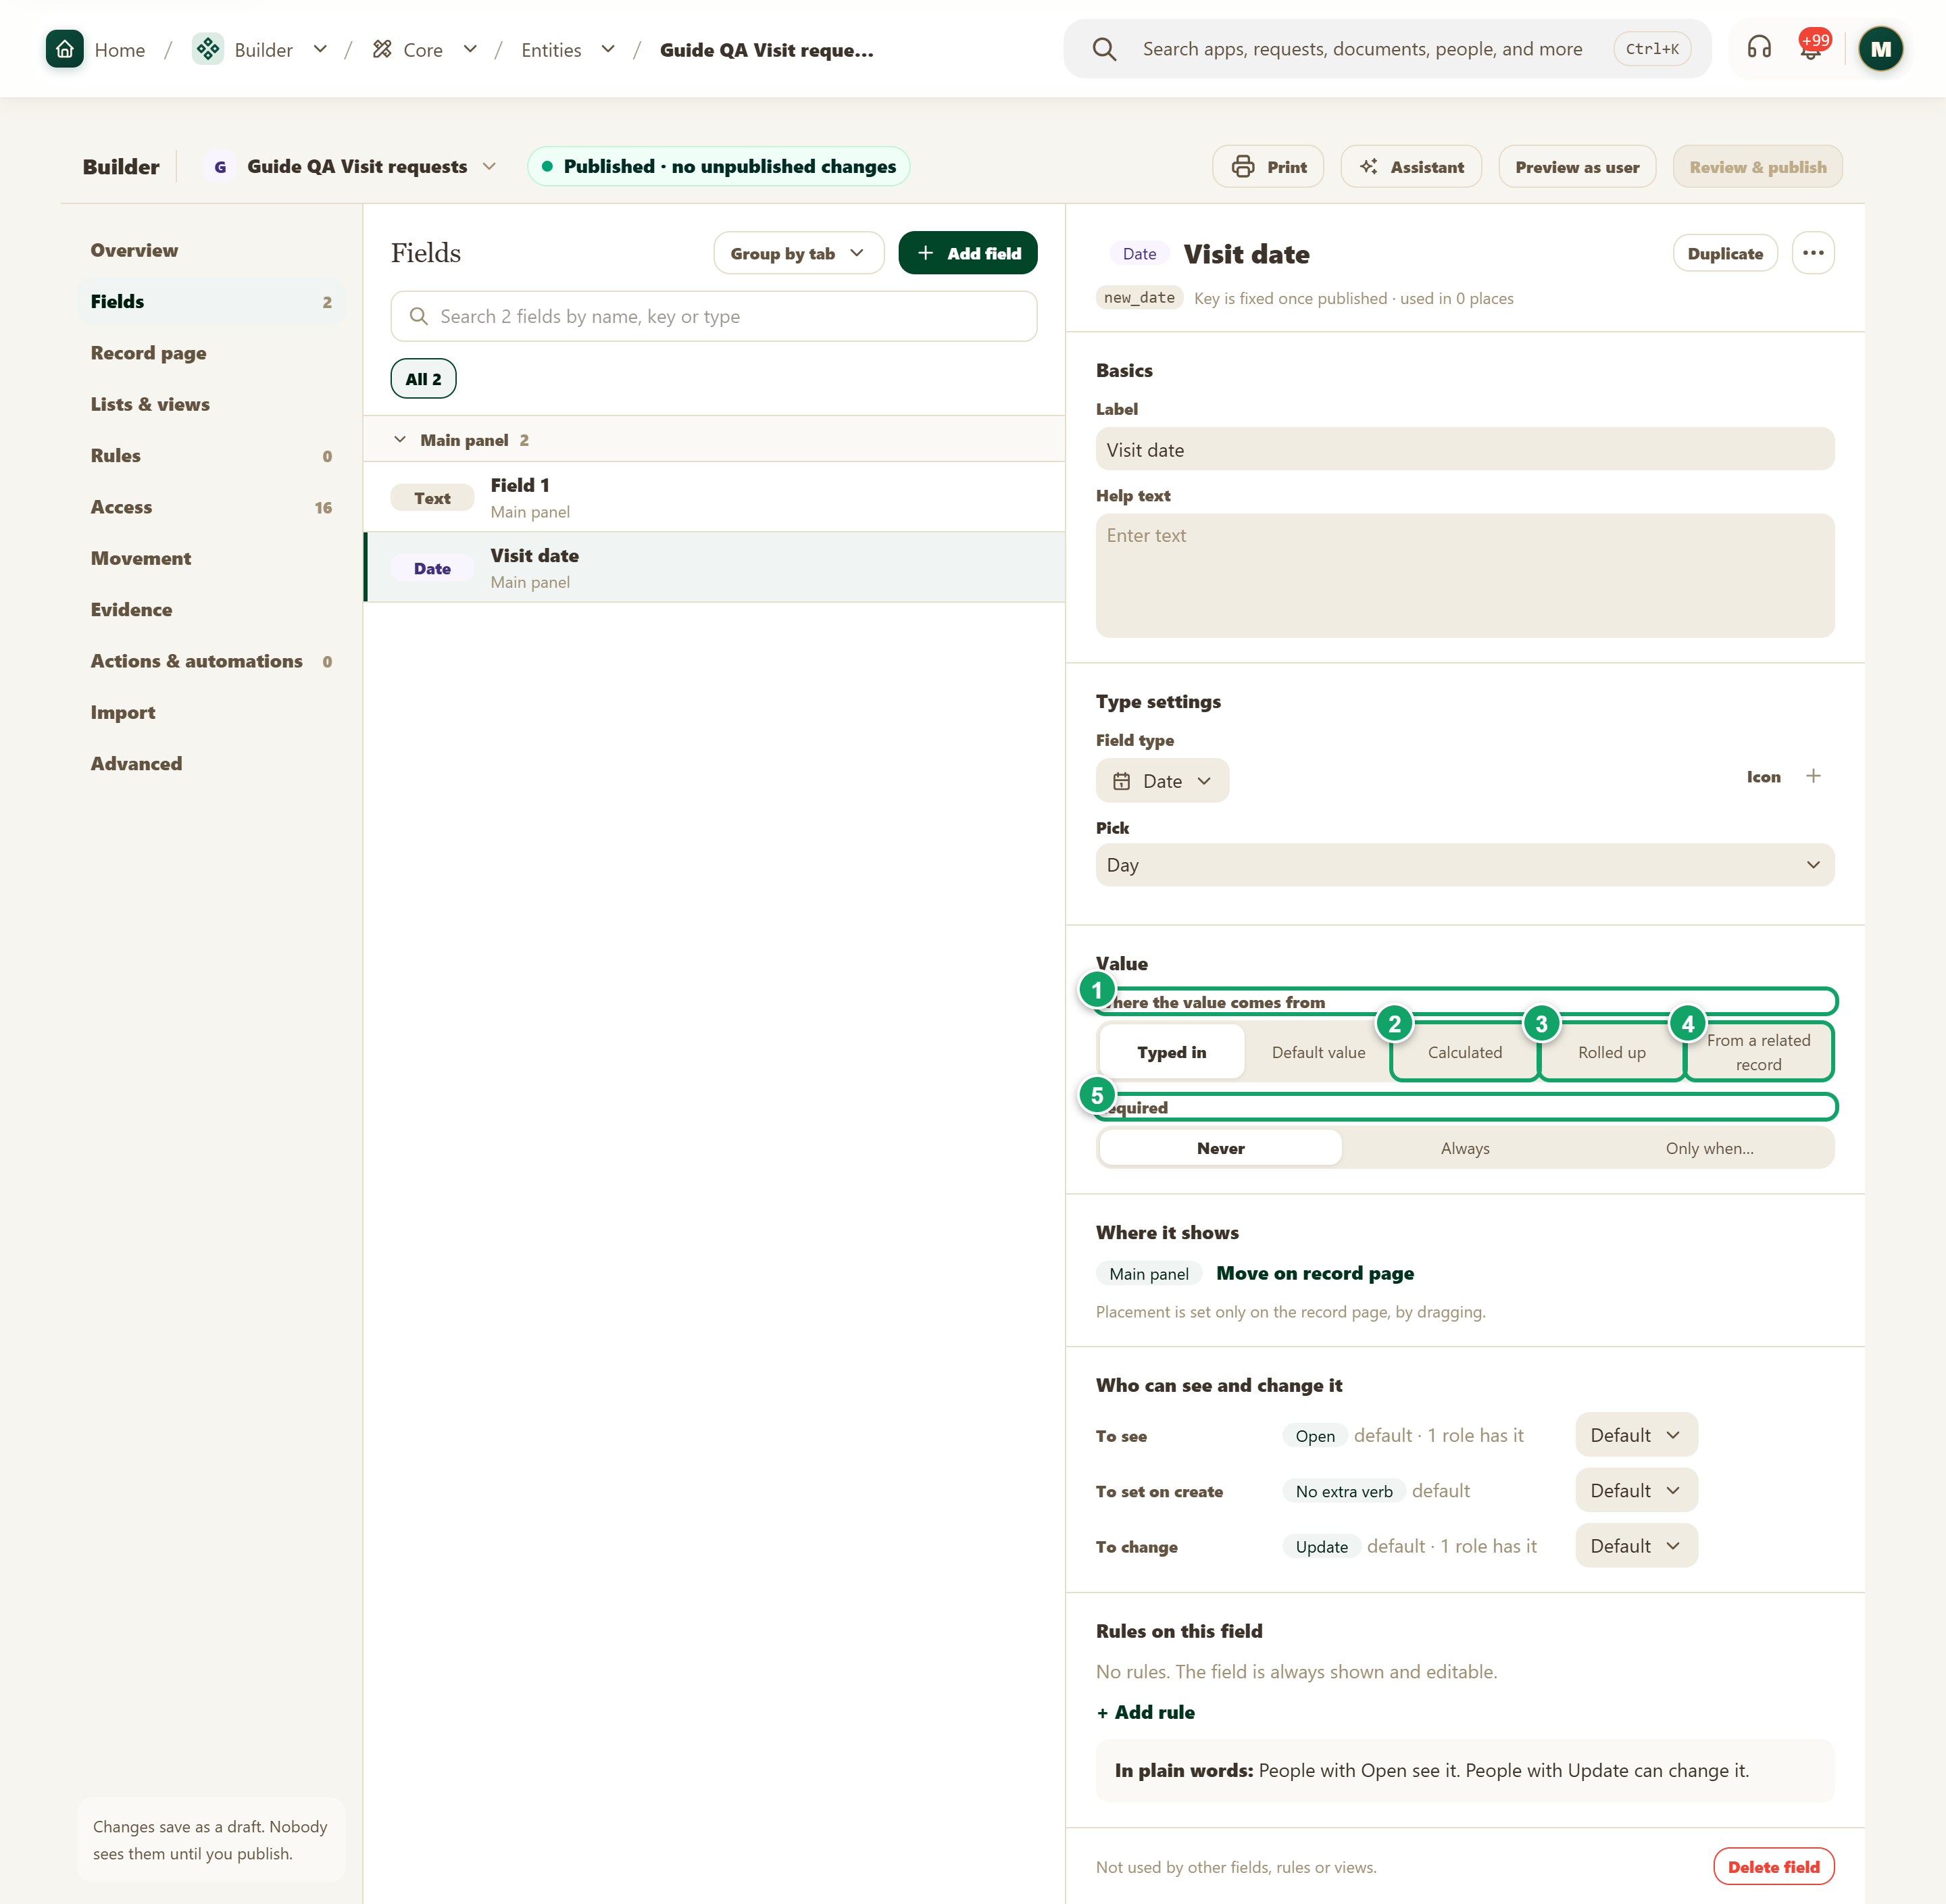
\includegraphics[width=0.95\linewidth,height=0.72\textheight,keepaspectratio]{figures/screens/ch06-ws-value-source-en.png}
\caption{The “Where the value comes from” setting in a date field’s panel}
\label{fig:builder-field-values-screen}
\shotnote{The image shows the settings of the “Visit date” field in the test type, with the “Value” section and its options. It shows that the value source and whether the field is required are set in one place in the field panel. ① “Where the value comes from”. ② “Calculated”: the value is a formula result. ③ “Rolled up”: the value comes from linked records. ④ “From a related record”: the value comes from a field of a related record. ⑤ “Required”: when saving is blocked if the field is empty.}
\end{figure}

\begin{table}[H]
\centering
\caption{“Where the value comes from” options}
\label{tab:builder-field-values-sources}
\begin{tabularx}{\linewidth}{R{3.6cm} Y}
\rcHeaderRow
\thh{Option} & \thh{When to use it}\\
Typed in & The user types the value. This is the usual choice for most fields.\\
Default value & The value starts with one you choose and the user can change it, such as an initial status or today's date.\\
Calculated & The value is calculated by a formula from fields of the same record or its related records, such as quantity times price. In “Automatic refresh” you choose whether it is recalculated only when the record's data changes, or daily, weekly or monthly.\\
Rolled up & The value is gathered from the records that link to this record, or from its linked tasks: their count, or the sum, average, lowest or highest of a field, or the earliest and latest date.\\
From a related record & Shows the value of a field in a related record, such as the branch's province, and updates automatically when it changes there.\\
\end{tabularx}
\end{table}

\subsection{Building a rolled-up value}

When you choose “Rolled up”, an editor guides you step by step. You start with “Roll up from” and choose the records that link to this record, then choose the operation in “Calculate”, such as “Count”, “Sum” or “Average”. You can narrow the records with conditions in “Only include records where”, and divide the result by the number of records to show it as a percentage. The preview shows the result on a sample record, then you press “Use this rollup”.

\subsection{Showing a value from a related record}

When you choose “From a related record”, the “Where does the value come from?” window appears: you choose the relation, then the field to show. If the record has more than one related record, “Calculation” decides whether to show the first, a list of values, their count or their sum. You also decide what shows when there is no related record: a blank field or text you write. Archived records are not counted, and this field cannot be required; make the relation field itself required instead.

\subsection{Required: never, always or only when}

The “Required” setting decides when saving the record is blocked if the field is empty: “Never”, “Always”, or “Only when…” for a given situation. The last option takes you to “Rules” to build a “Require” rule with its condition. The setting is not available for calculated and lookup fields, because users do not type their values.

\begin{figure}[H]
\centering
\begin{tikzpicture}[node distance=0.5cm]
\node[stepBox] (a) {Choose Rolled up};
\node[stepBox,below=of a] (b) {Roll up from};
\node[stepBox,below=of b] (c) {Calculate};
\node[stepBox,below=of c] (d) {Only include records where};
\node[stepBox,below=of d] (e) {Preview on a record};
\node[stepBox,below=of e] (f) {Use this rollup};
\draw[flowsTo] (a) -- (b);
\draw[flowsTo] (b) -- (c);
\draw[flowsTo] (c) -- (d);
\draw[flowsTo] (d) -- (e);
\draw[flowsTo] (e) -- (f);
\end{tikzpicture}
\rclegend
\caption{Building a rolled-up value}
\label{fig:builder-field-values-flow}
\shotnote{The diagram follows the editor's own order: you choose the records first because the available operations depend on their fields, then the calculation, then the conditions that narrow them. The preview comes before saving so you see the number on a real record and catch a wrong condition or operation before the team sees it.}
\end{figure}

\subsection{Steps and check}
\begin{enumerate}
\item Add a field of the right type for the result, such as “Number” for a count or sum, then open “Value” and choose “Where the value comes from”.
\item For a calculated value, choose “Calculated”, write the formula in the editor, then choose the suitable “Automatic refresh”.
\item For a rolled-up value, follow the editor from “Roll up from” to “Use this rollup”.
\item For a value from a related record, make sure a “Relation” field exists, then choose “From a related record” and select the relation and the field.
\item Publish the changes, then open a record linked to other records and compare the value with what you expect.
\end{enumerate}

\textbf{Check and recovery:} the value should appear without anyone typing it, and change when its sources change. If “Before you publish” shows the field's name followed by “can’t be calculated”, the formula points to a field that does not exist; press “Fix formula” and choose the right field. If you switch a lookup field to “Typed in”, its current values stay but no longer update.

\clearpage
\section{Status fields and lifecycle rules}
\label{sec:builder-feature-lifecycle}

A “Status” field follows the work stages of a status template, such as “New”, then “Under review”, then “Approved”. “Lifecycle rules” add controls to it: when a move from one status to another is allowed, who may not make it, which fields are set automatically during the move, and whether the record is locked in a given status. So following the procedure does not depend on employees remembering it.

\textbf{Path and who uses it:} Builder workspace → “Fields” → choose the status field → “Lifecycle rules”. The rules need a “Fixed template” in the field's settings and are not available on built-in record types. Status templates themselves are explained in the Tasks chapter, on page \ref{sec:tasks-feature-statuses}.

\begin{rcnote}[Example: Horizon]
The administrator forbids the requester from moving a “Visit requests” record to “Approved”, so Omar Haddad cannot approve his own request. They add an effect that writes the approval date and approver, then lock the approved request so its data does not change after Sarah Al-Khatib approves it.
\end{rcnote}

\begin{table}[H]
\centering
\caption{What you set for each transition}
\label{tab:builder-lifecycle-transitions}
\begin{tabularx}{\linewidth}{R{3.6cm} Y}
\rcHeaderRow
\thh{Setting} & \thh{Meaning}\\
Only when & A condition that must hold before the transition, such as a visit date being present.\\
Message when blocked & The text the user sees when the condition is not met, so they know what is missing.\\
Can't be done by members in & Member fields in the record whose people may not make the transition, such as the requester.\\
When the transition runs & Effects written in the same save: “Set” a field to “Now”, “Current member”, a fixed value or an expression, or “Clear” it. These fields are written even when the record is locked.\\
\end{tabularx}
\end{table}

\begin{table}[H]
\centering
\caption{What you set for each status}
\label{tab:builder-lifecycle-states}
\begin{tabularx}{\linewidth}{R{3.6cm} Y}
\rcHeaderRow
\thh{Setting} & \thh{Meaning}\\
Editing & “Not locked”, “Locked”, or “Locked except…” fields that stay editable.\\
Block delete & Prevents deleting the record while it is in this status.\\
Also lock records pointing here & Also locks the records linked to it, such as the lines of an approved request.\\
Freeze a version on entering & Saves a copy of the record under a name you choose when it enters the status, to return to later.\\
\end{tabularx}
\end{table}

\begin{rcwarn}[Status changes only through transitions]
When “Status changes only through transitions” is on, forms, imports and automations cannot set the status directly, and every new record starts at the first status. If an automation changes the status, review it before turning this option on.
\end{rcwarn}

\begin{figure}[H]
\centering
\begin{tikzpicture}[node distance=0.5cm]
\node[stepBox] (a) {Fixed status template};
\node[stepBox,below=of a] (b) {Transition conditions};
\node[stepBox,below=of b] (c) {Who may not move it};
\node[stepBox,below=of c] (d) {Transition effects};
\node[stepBox,below=of d] (e) {Locking per status};
\draw[flowsTo] (a) -- (b);
\draw[flowsTo] (b) -- (c);
\draw[flowsTo] (c) -- (d);
\draw[flowsTo] (d) -- (e);
\end{tikzpicture}
\rclegend
\caption{Setting a record's lifecycle}
\label{fig:builder-lifecycle-flow}
\shotnote{The diagram starts with the fixed template because all rules are built on its transitions and do not appear without it. Each transition is then set on its own, and locking comes last because it protects the record after it reaches the status, giving the order: when the record moves, who moves it, and what happens next.}
\end{figure}

\subsection{Steps and check}
\begin{enumerate}
\item Open the status field in “Fields”, and in “Type settings” choose “Fixed template” and the suitable status template.
\item Open “Lifecycle rules”, choose the transition to set, add its condition in “Only when” and its message in “Message when blocked”.
\item In “Can't be done by members in”, choose the requester field if requesters may not approve their own request.
\item In “When the transition runs”, add an effect that writes the date or the current member, then set editing lock for the final status.
\item Publish the changes and try the transition with a test record, once with the condition missing and once with it met.
\end{enumerate}

\textbf{Check and recovery:} the transition should be blocked with your message when the condition is missing, and go through and write the chosen fields when it is met. If “Lifecycle rules” do not appear, choose “Fixed template” first; if the type is built into the system, these rules are not available for it.

\clearpage
\section{Record page}
\label{sec:builder-feature-record-page}

The record page is what a user sees when opening a single record. The “Record page” section arranges the fields into tabs and sections, so related information appears together instead of in one long list. You can also add blocks at the top of the first tab and lists of related records.

\textbf{Path and who uses it:} record type → “Record page”. Used by whoever builds the type, after adding its fields.

\begin{rcnote}[Example: Horizon]
The system administrator gives the visit request page two tabs: “Request” for the branch, date and purpose, and “Review” for Sarah Al-Khatib's notes and decision, so Omar Haddad finds what concerns him in the first tab. They create the two tabs from ② and then drag the fields into them.
\end{rcnote}

\begin{figure}[H]
\centering
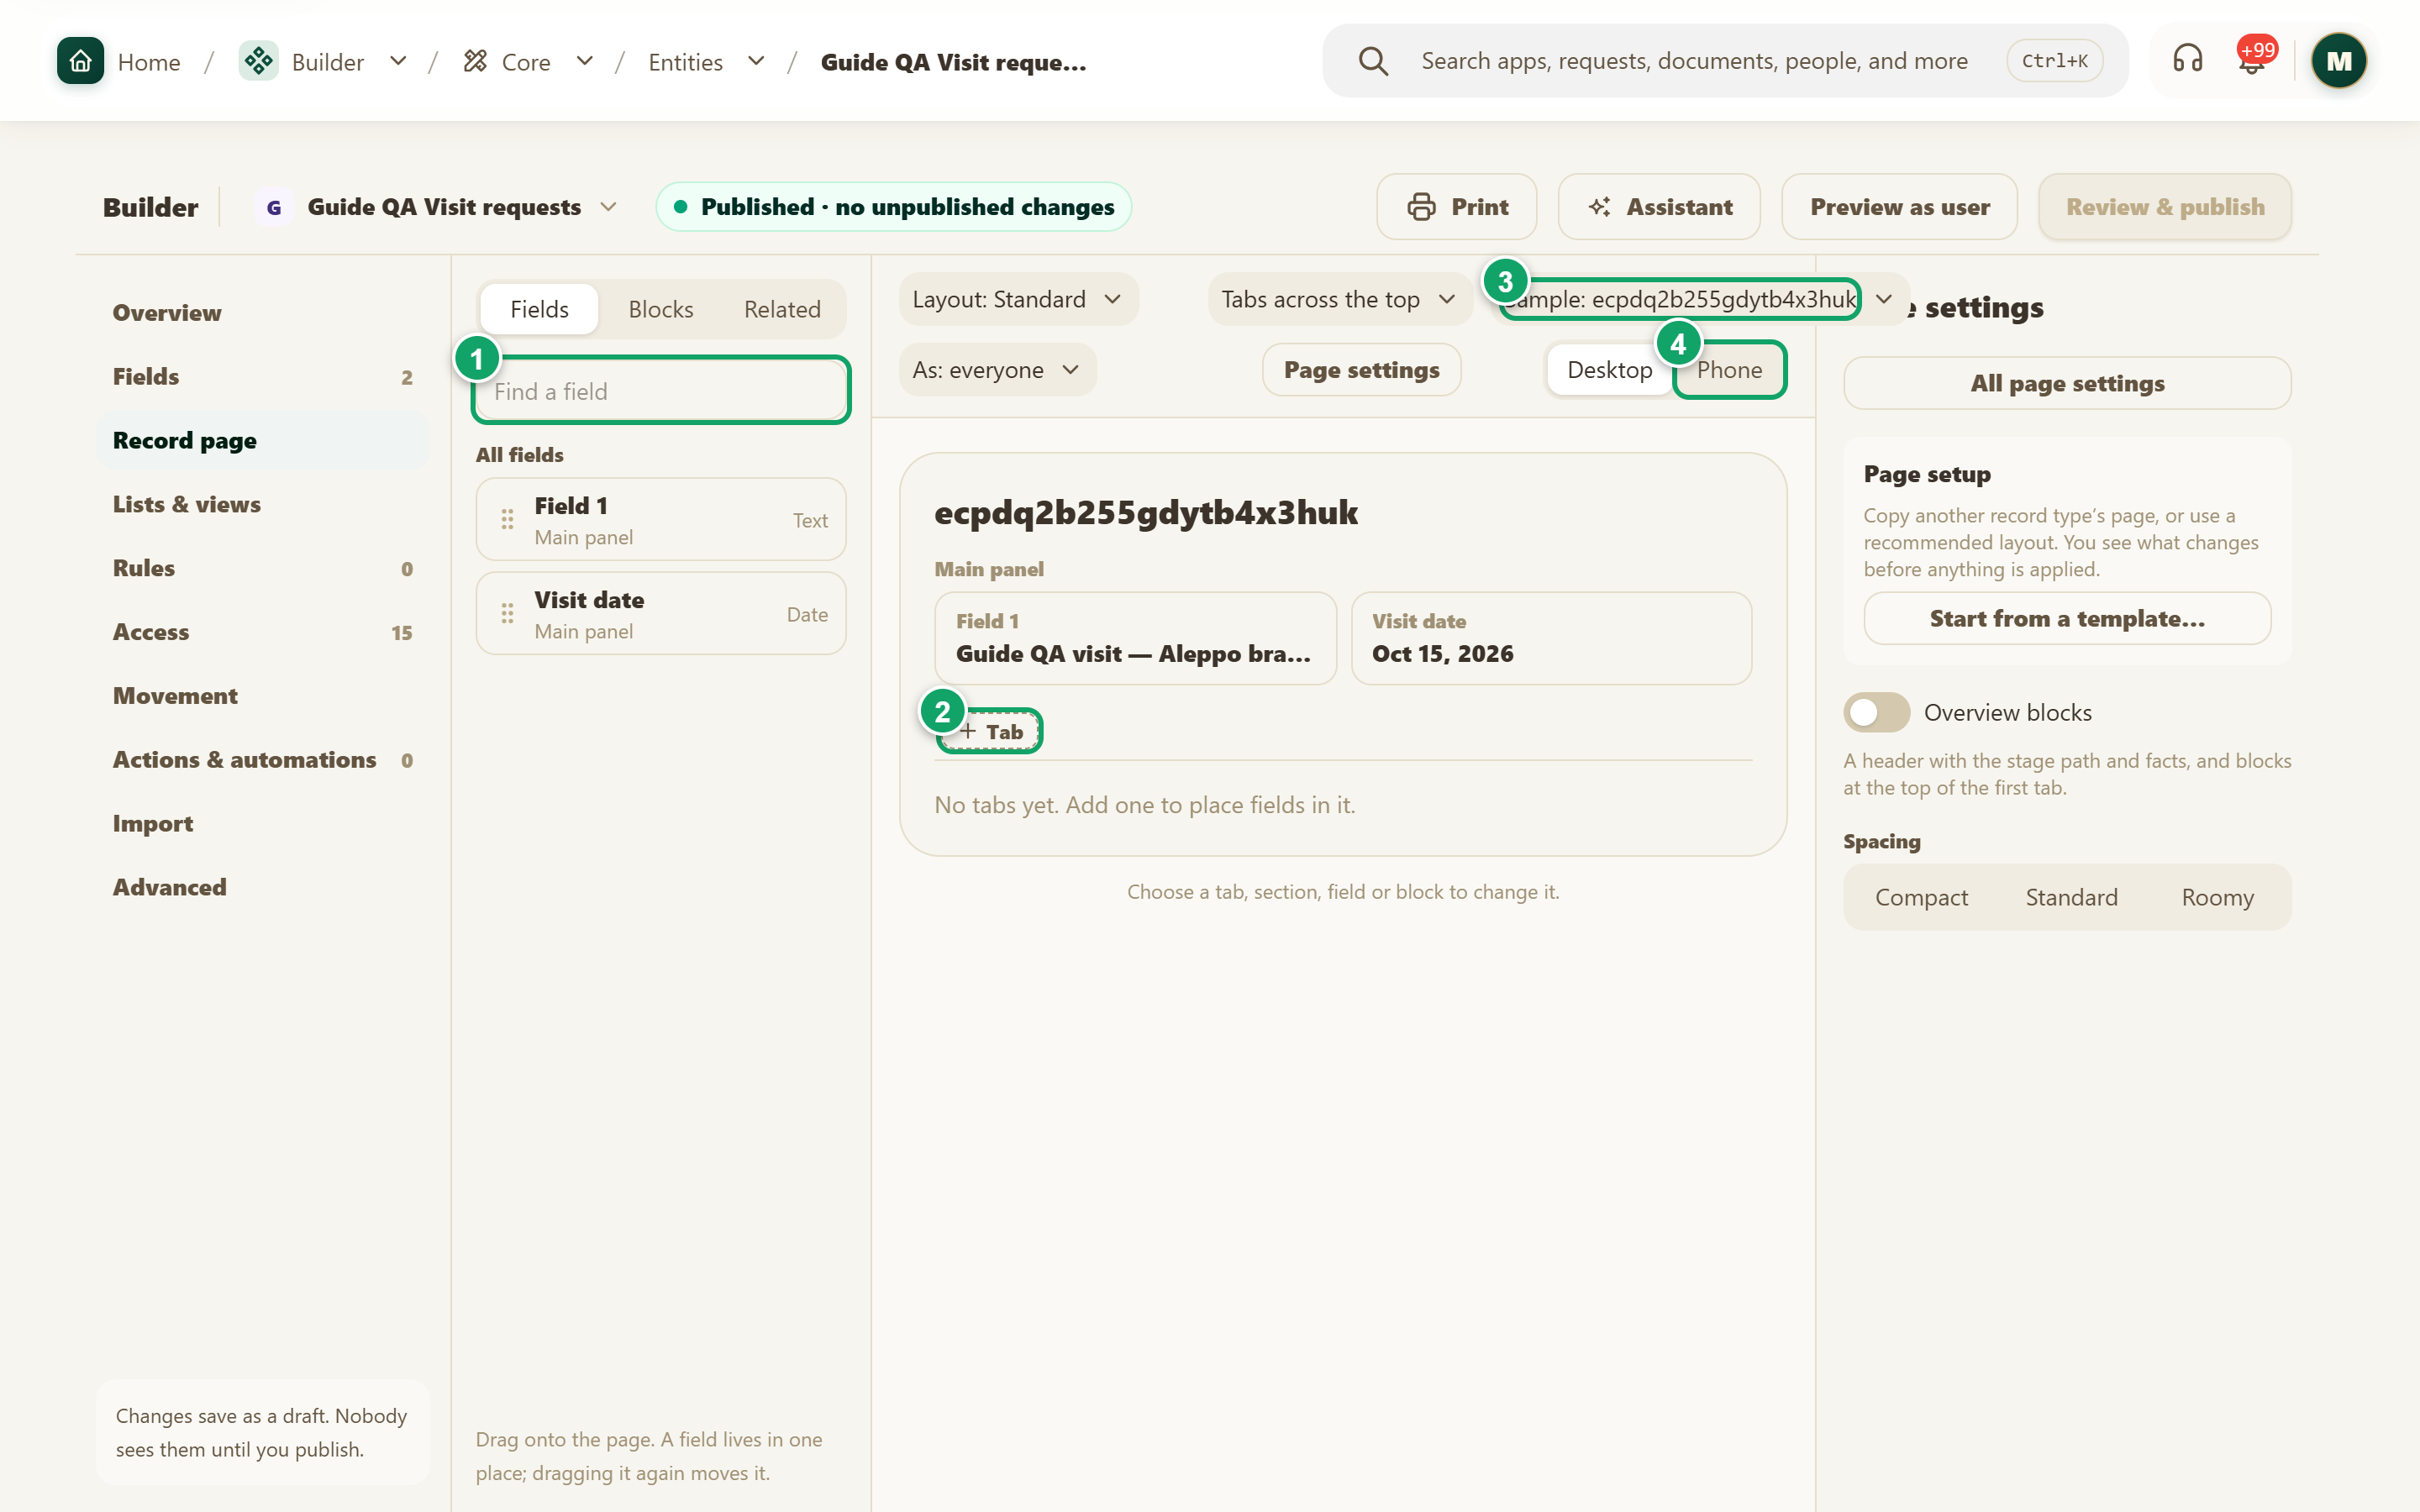
\includegraphics[width=0.95\linewidth,height=0.72\textheight,keepaspectratio]{figures/screens/ch06-ws-record-page-en.png}
\caption{The “Record page” section with a real record preview}
\label{fig:builder-record-page-screen}
\shotnote{The section shows the page parts on one side and the page itself in the middle with a test record’s values, so you see the arrangement before publishing. ① “Find a field”: finds the field you want to drag onto the page. ② “Tab”: adds a tab to hold sections and fields. ③ “Sample”: the record used to preview the page. ④ “Phone”: shows the page as it appears on a small screen.}
\end{figure}


\begin{table}[H]
\centering
\caption{What do you find here?}
\label{tab:builder-record-page-data}
\begin{tabularx}{\linewidth}{R{3.6cm} Y}
\rcHeaderRow
\thh{Section} & \thh{Content and action}\\
Tabs and sections & Create a “New tab” or “New section”, then drag fields into it. A field has one place on the page; dragging it again moves it.\\
Page parts & Groups “All fields”, “Blocks” and “Related” lists, and shows the fields that are “Not on the page yet”.\\
Layout and header & Chooses the page shape, tabs or a section list, with header settings and overview blocks.\\
Preview & Shows the page with a sample of a real record, as a chosen role sees it, on desktop or phone.\\
\end{tabularx}
\end{table}

\begin{figure}[H]
\centering
\begin{tikzpicture}[node distance=0.5cm]
\node[entity] (page) {Record page};
\node[entity,below=0.7cm of page] (tab) {Tab};
\node[entity,below=0.7cm of tab] (section) {Section};
\node[entity,below=0.7cm of section] (field) {Field};
\draw[dependsOn] (page) -- (tab);
\draw[dependsOn] (tab) -- (section);
\draw[dependsOn] (section) -- (field);
\end{tikzpicture}
\rclegend
\caption{How the page is arranged}
\label{fig:builder-record-page-tree}
\shotnote{The figure shows the levels of arrangement: the page holds tabs, each tab holds sections and each section holds fields. So you create the tab and section first and then drag fields into them; a field you place in no section is still saved but does not appear on the page.}
\end{figure}

\subsection{Steps and check}
\begin{enumerate}
\item Open the record type and choose “Record page”.
\item Create the tabs the work needs, then add one or more sections to each tab.
\item Drag each field from “Page parts” into the right section, and check “Not on the page yet” so no important field is left off the page.
\item Switch the preview size to “Phone” to make sure the page is clear on a small screen.
\end{enumerate}

\textbf{Check and recovery:} the preview should show the fields in the tabs and sections you chose. If a field does not appear, find it under “Not on the page yet” and drag it into a section; if a message says a field is placed in a tab that does not exist, move it to an existing tab.

\clearpage
\section{Overview blocks and layouts}
\label{sec:builder-feature-record-page-blocks}

Besides fields, a record page can open with a summary of what matters most: the stage path, key figures and what needs attention. These summaries are built from “Overview blocks”, which show at the top of the first tab. “Layouts” are saved arrangements of the page that you choose between by a value in the record, so each kind of record gets the arrangement that suits it best.

\textbf{Path and who uses it:} Builder workspace → “Record page” → “Page settings” to turn on overview blocks, then “Page parts” → “Blocks” to add them. Layouts are under “Manage layouts…”. Used by the person who builds the type once its fields are settled.

\begin{rcnote}[Example: Horizon]
The administrator adds a “Metrics” block to the “Visit requests” page showing how many days the request has been open, and a “Needs attention” block that alerts Sarah Al-Khatib to a request waiting more than three days for review.
\end{rcnote}

\begin{figure}[H]
\centering
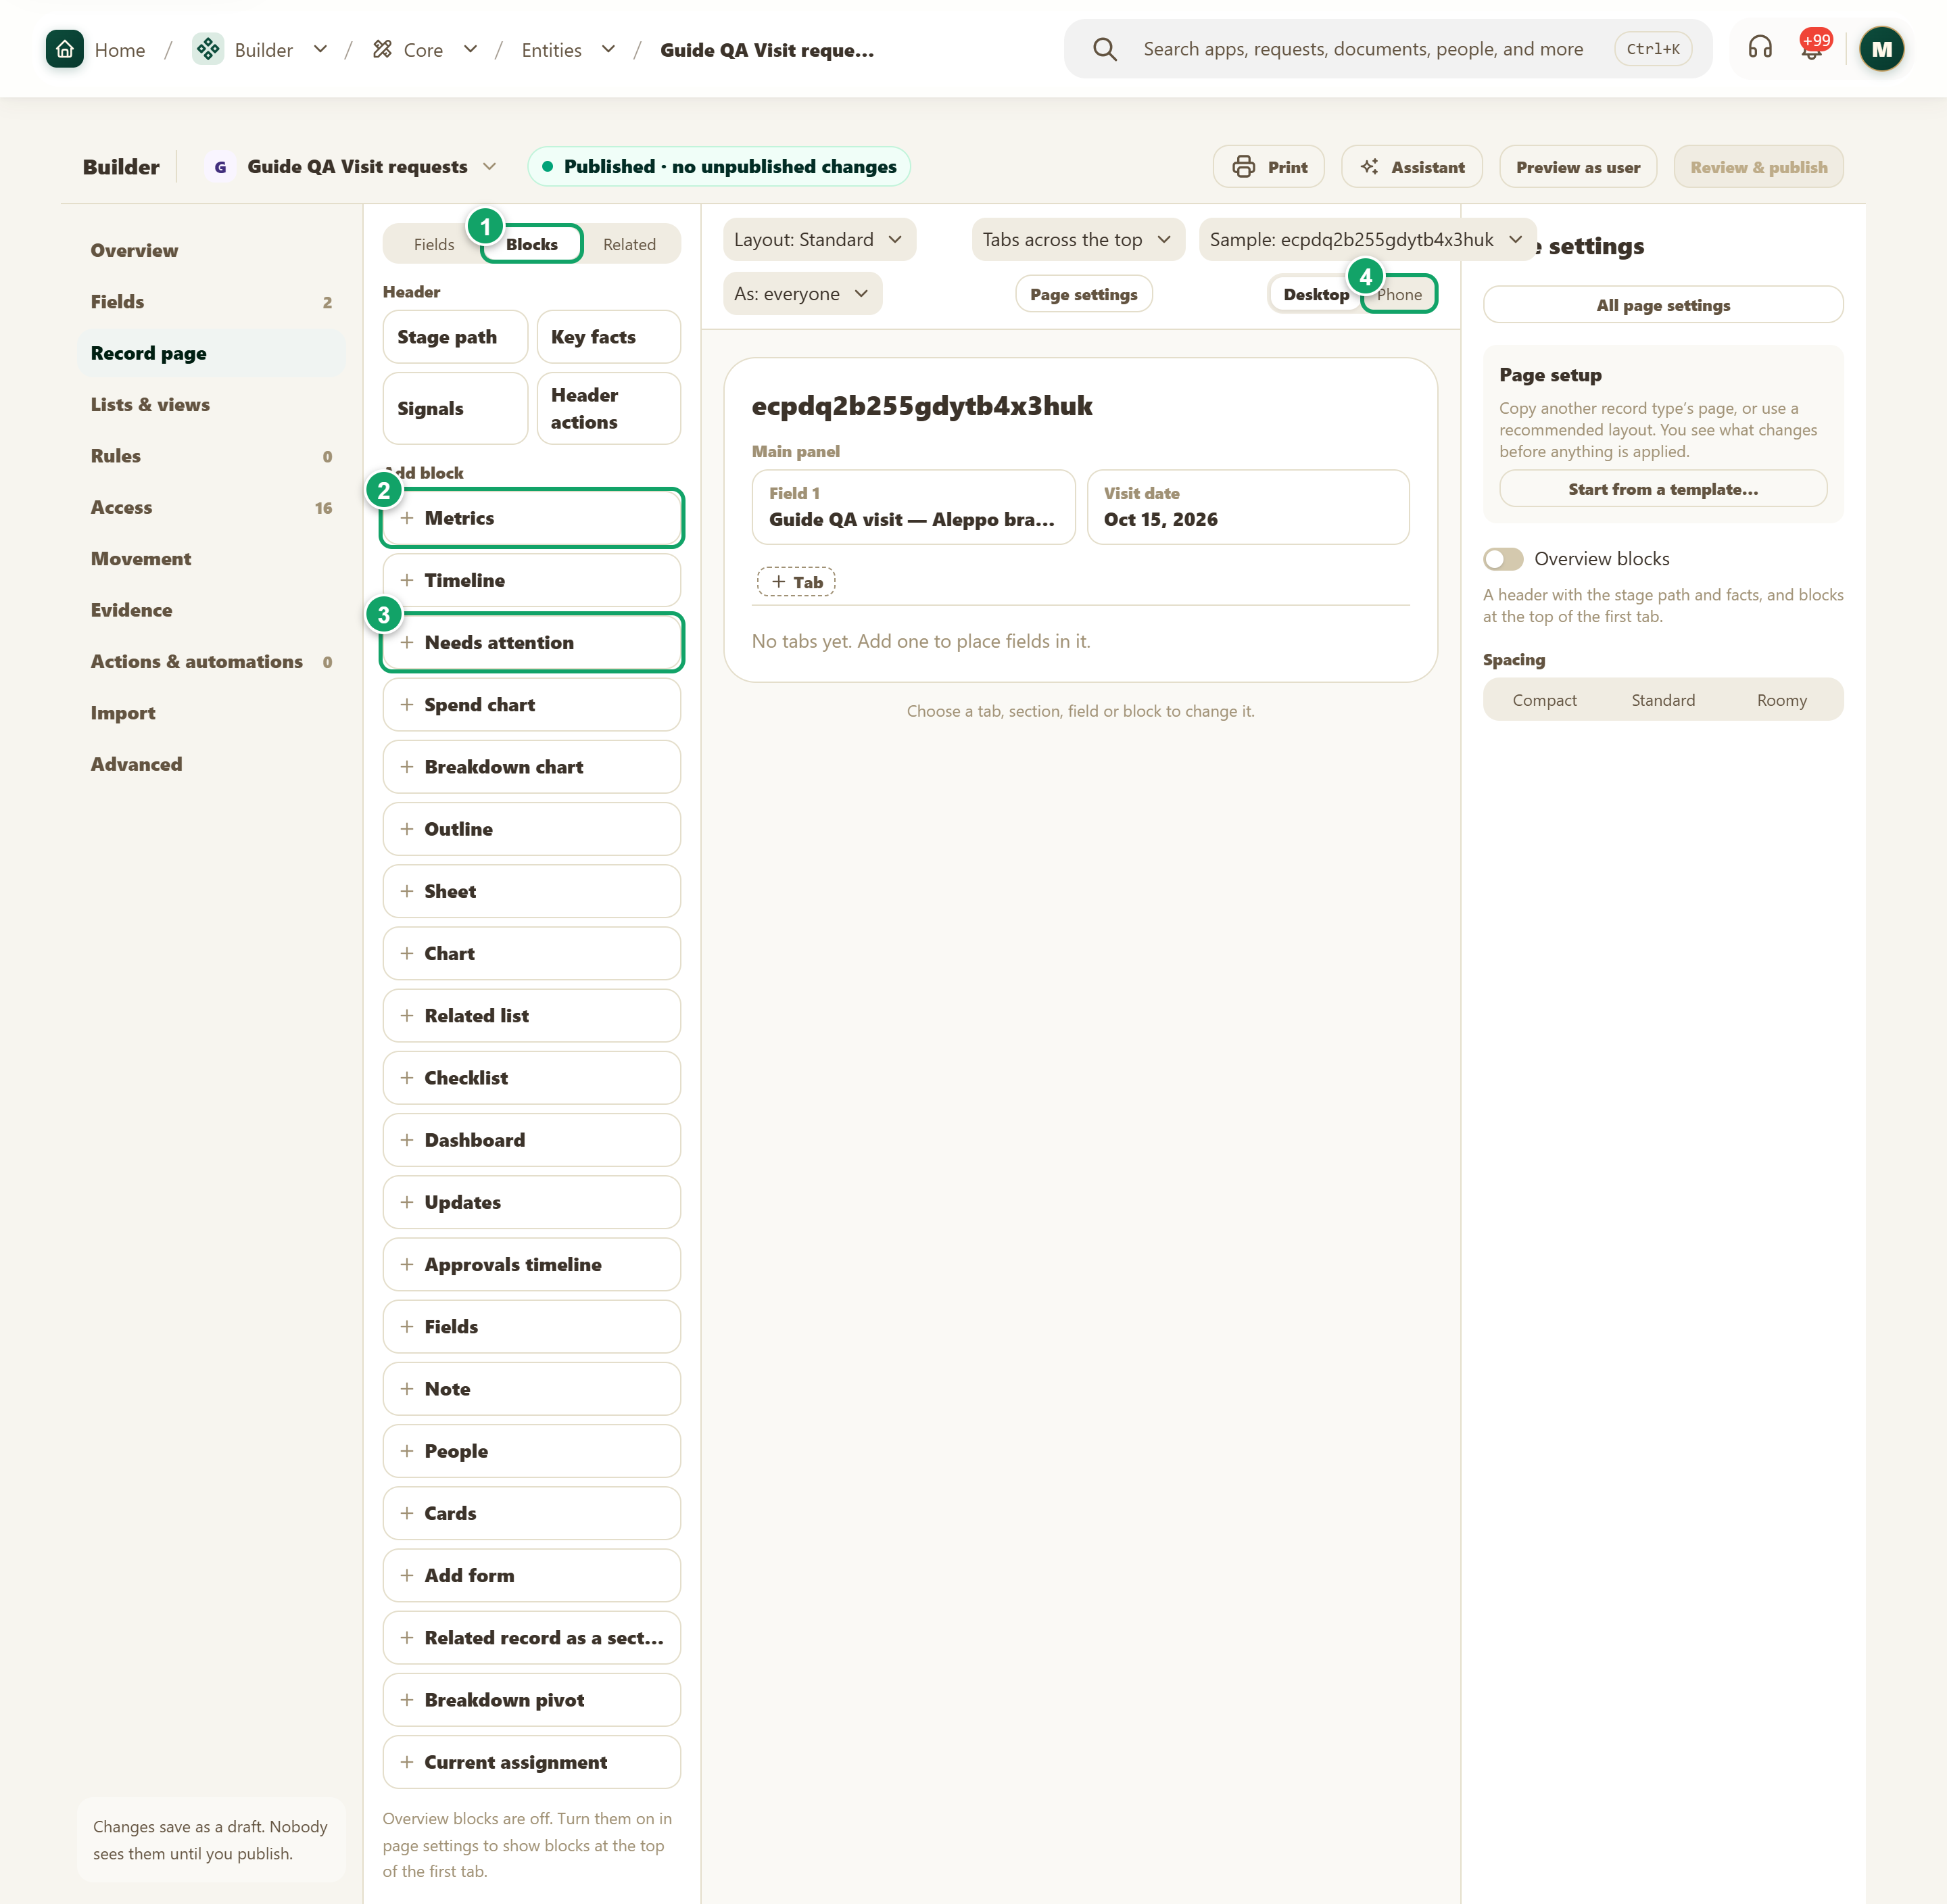
\includegraphics[width=0.95\linewidth,height=0.72\textheight,keepaspectratio]{figures/screens/ch06-ws-blocks-en.png}
\caption{The “Blocks” tab in “Page parts”}
\label{fig:builder-record-page-blocks-screen}
\shotnote{The image shows the “Record page” section with the blocks tab open, listing every block that can sit at the top of the first tab, with the preview beside it. It helps you choose a block and see its effect before publishing. ① “Blocks”. ② “Metrics”: key figures about the record. ③ “Needs attention”: alerts from rules you set. ④ “Phone”: shows the preview at phone size.}
\end{figure}

\begin{table}[H]
\centering
\caption{Page parts}
\label{tab:builder-record-page-blocks-parts}
\begin{tabularx}{\linewidth}{R{3.6cm} Y}
\rcHeaderRow
\thh{Tab} & \thh{What you add from it}\\
Fields & You drag the field to its place on the page. Unplaced fields show under “Not on the page yet”; a field lives in one place, so dragging it again moves it.\\
Blocks & You choose a block to set it up, then add it at the top of the first tab.\\
Related & Lists of related records, placed from the relation field of the linked record type.\\
\end{tabularx}
\end{table}

\begin{table}[H]
\centering
\caption{The most used blocks}
\label{tab:builder-record-page-blocks-kinds}
\begin{tabularx}{\linewidth}{R{3.6cm} Y}
\rcHeaderRow
\thh{Block} & \thh{What it shows}\\
Metrics & Key figures, such as progress, used of total, or a slipped date.\\
Needs attention & Alerts from rules you set, with a “Critical”, “Warning” or “Information” tone, showing the count or the list of matching records.\\
Timeline & Dates and milestones from the record and its related records on a timeline.\\
Related list and Cards & Related records as a table or cards inside the page.\\
Approvals timeline and Updates & The history of approvals and the latest updates on the record.\\
Note, Fields and People & Fixed text, a group of fields, or the people linked to the record.\\
Chart and Dashboard & A chart from the record's data, or a ready dashboard.\\
\end{tabularx}
\end{table}

\subsection{Preview and layouts}

The preview shows the page with a sample record chosen in “Sample”; you can view it “As” a given role, at “Desktop” or “Phone” size. “Manage layouts…” opens the “Layouts” window: a layout keeps section styles and columns, spacing, the header and overview blocks, while tabs, sections and where fields sit are shared by every layout. There you set the default layout, or pick the layout from a field's value in the record.

\begin{figure}[H]
\centering
\begin{tikzpicture}[node distance=0.5cm]
\node[stepBox] (a) {Turn on overview blocks};
\node[stepBox,below=of a] (b) {Add a block};
\node[stepBox,below=of b] (c) {Set the block and its width};
\node[stepBox,below=of c] (d) {Preview as a role};
\node[stepBox,below=of d] (e) {Review and publish};
\draw[flowsTo] (a) -- (b);
\draw[flowsTo] (b) -- (c);
\draw[flowsTo] (c) -- (d);
\draw[flowsTo] (d) -- (e);
\end{tikzpicture}
\rclegend
\caption{Adding a block to the record page}
\label{fig:builder-record-page-blocks-flow}
\shotnote{The diagram starts by turning on overview blocks because the “Blocks” tab adds nothing before that. The role preview comes before publishing, because a block may show figures from records some roles may not see, so you confirm what each of them gets.}
\end{figure}

\subsection{Steps and check}
\begin{enumerate}
\item Open “Record page”, then “Page settings”, and turn on overview blocks.
\item Open “Page parts” → “Blocks”, choose the block, then press “Add block”.
\item Set the block: its title, width (“Full width”, “Two thirds” or “One third”) and what it shows, such as the “Needs attention” rules.
\item Change “As” to another role and “Preview size” to “Phone”, make sure the page is clear in both, then publish.
\end{enumerate}

\textbf{Check and recovery:} the block should show at the top of the first tab when a published record is opened. If “Overview blocks are off” appears, press “Turn on overview blocks” first. If the block is empty, try it on a record that has the data it relies on.

\clearpage
\section{Lists \& views}
\label{sec:builder-feature-lists}

The “Lists \& views” section decides how the type's records appear together when a user opens the list. You choose the views people can switch between, such as “Table”, “Kanban” or “Calendar”, the visible columns and the figures that summarize the list at the top. The “Inline cells” card offers “Edit cells in place”, so people edit table cells without opening each record, provided list views are on and they may change the field.

\textbf{Path and who uses it:} record type → “Lists \& views”. Used by whoever builds the type, and useful to everyone who follows the records daily.

\begin{rcnote}[Example: Horizon]
The system administrator shows visit requests in a “Table” with number, branch, date and status columns, and adds a “Calendar” by visit date, so Sarah Al-Khatib sees the week's visits at a glance. They start by turning on switch ① to choose the table and the calendar.
\end{rcnote}

\begin{figure}[H]
\centering
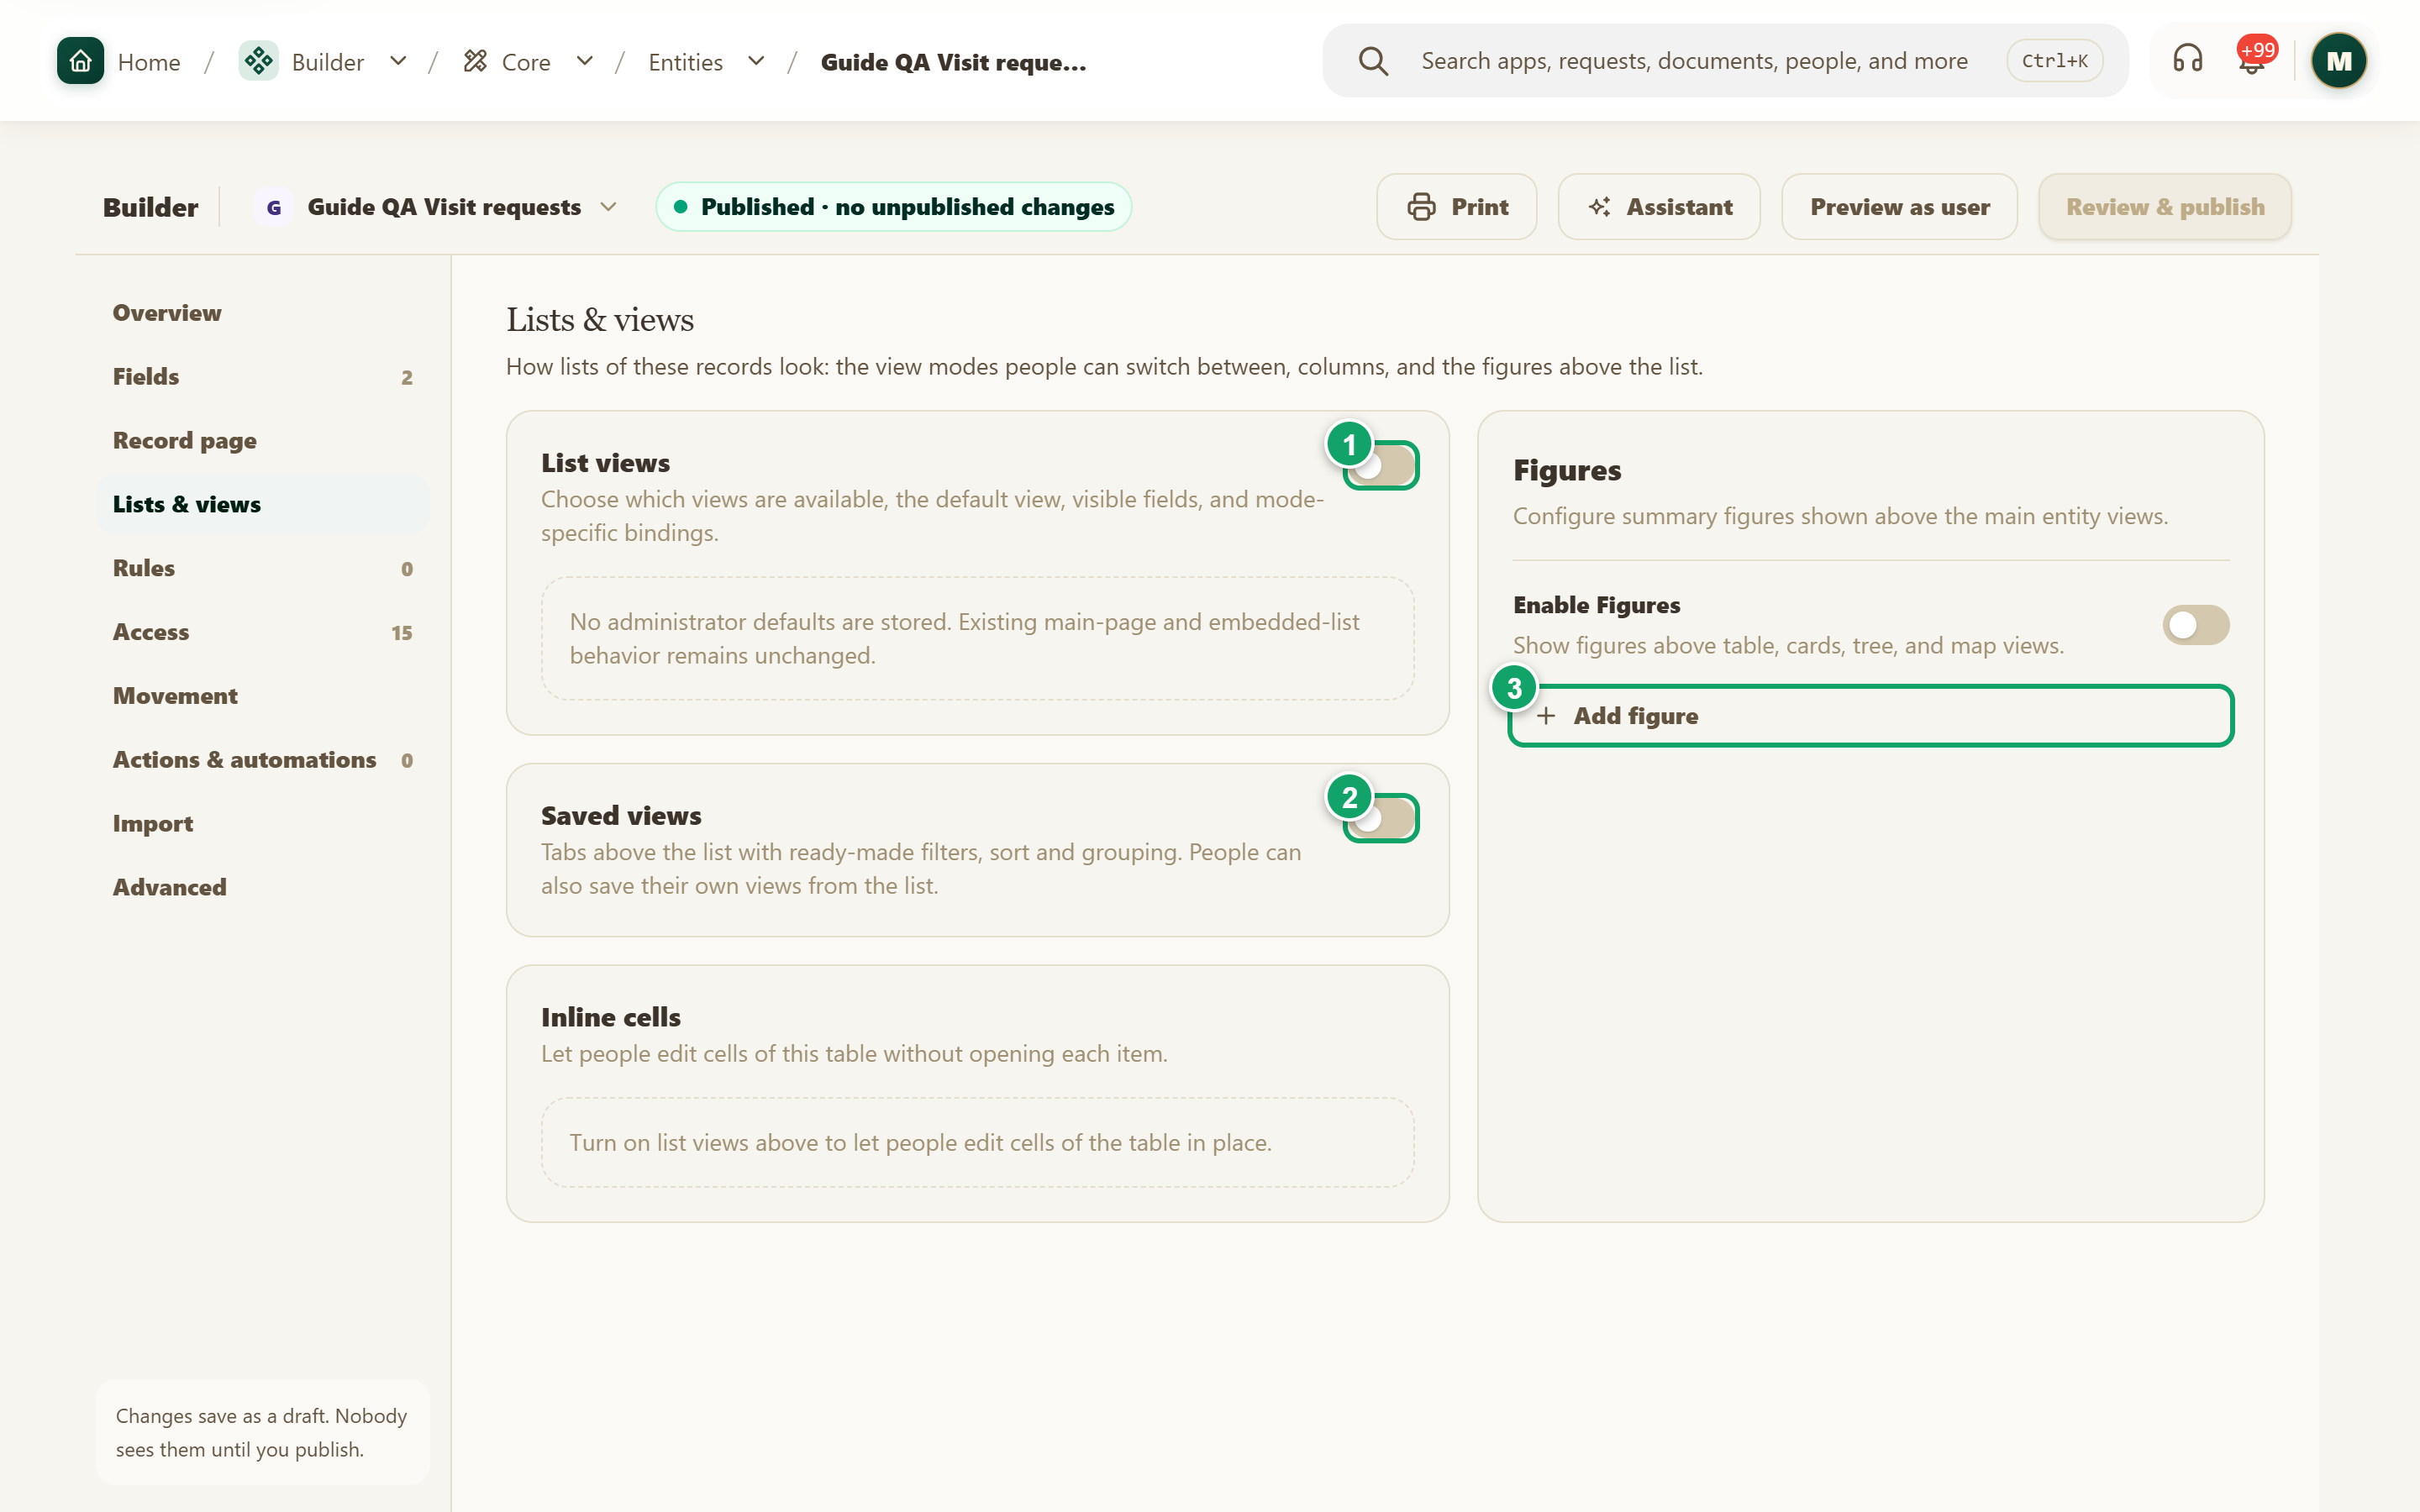
\includegraphics[width=0.95\linewidth,height=0.72\textheight,keepaspectratio]{figures/screens/ch06-ws-lists-en.png}
\caption{The “Lists \& views” section}
\label{fig:builder-lists-screen}
\shotnote{The section gathers what controls how the record list looks. All switches are off here, so the list uses its default setup. ① The “List views” switch: lets you choose the available and default views and the columns. ② The “Saved views” switch: adds ready-made tabs above the list. ③ “Add figure”: adds a summary number above the list.}
\end{figure}

\begin{figure}[H]
\centering
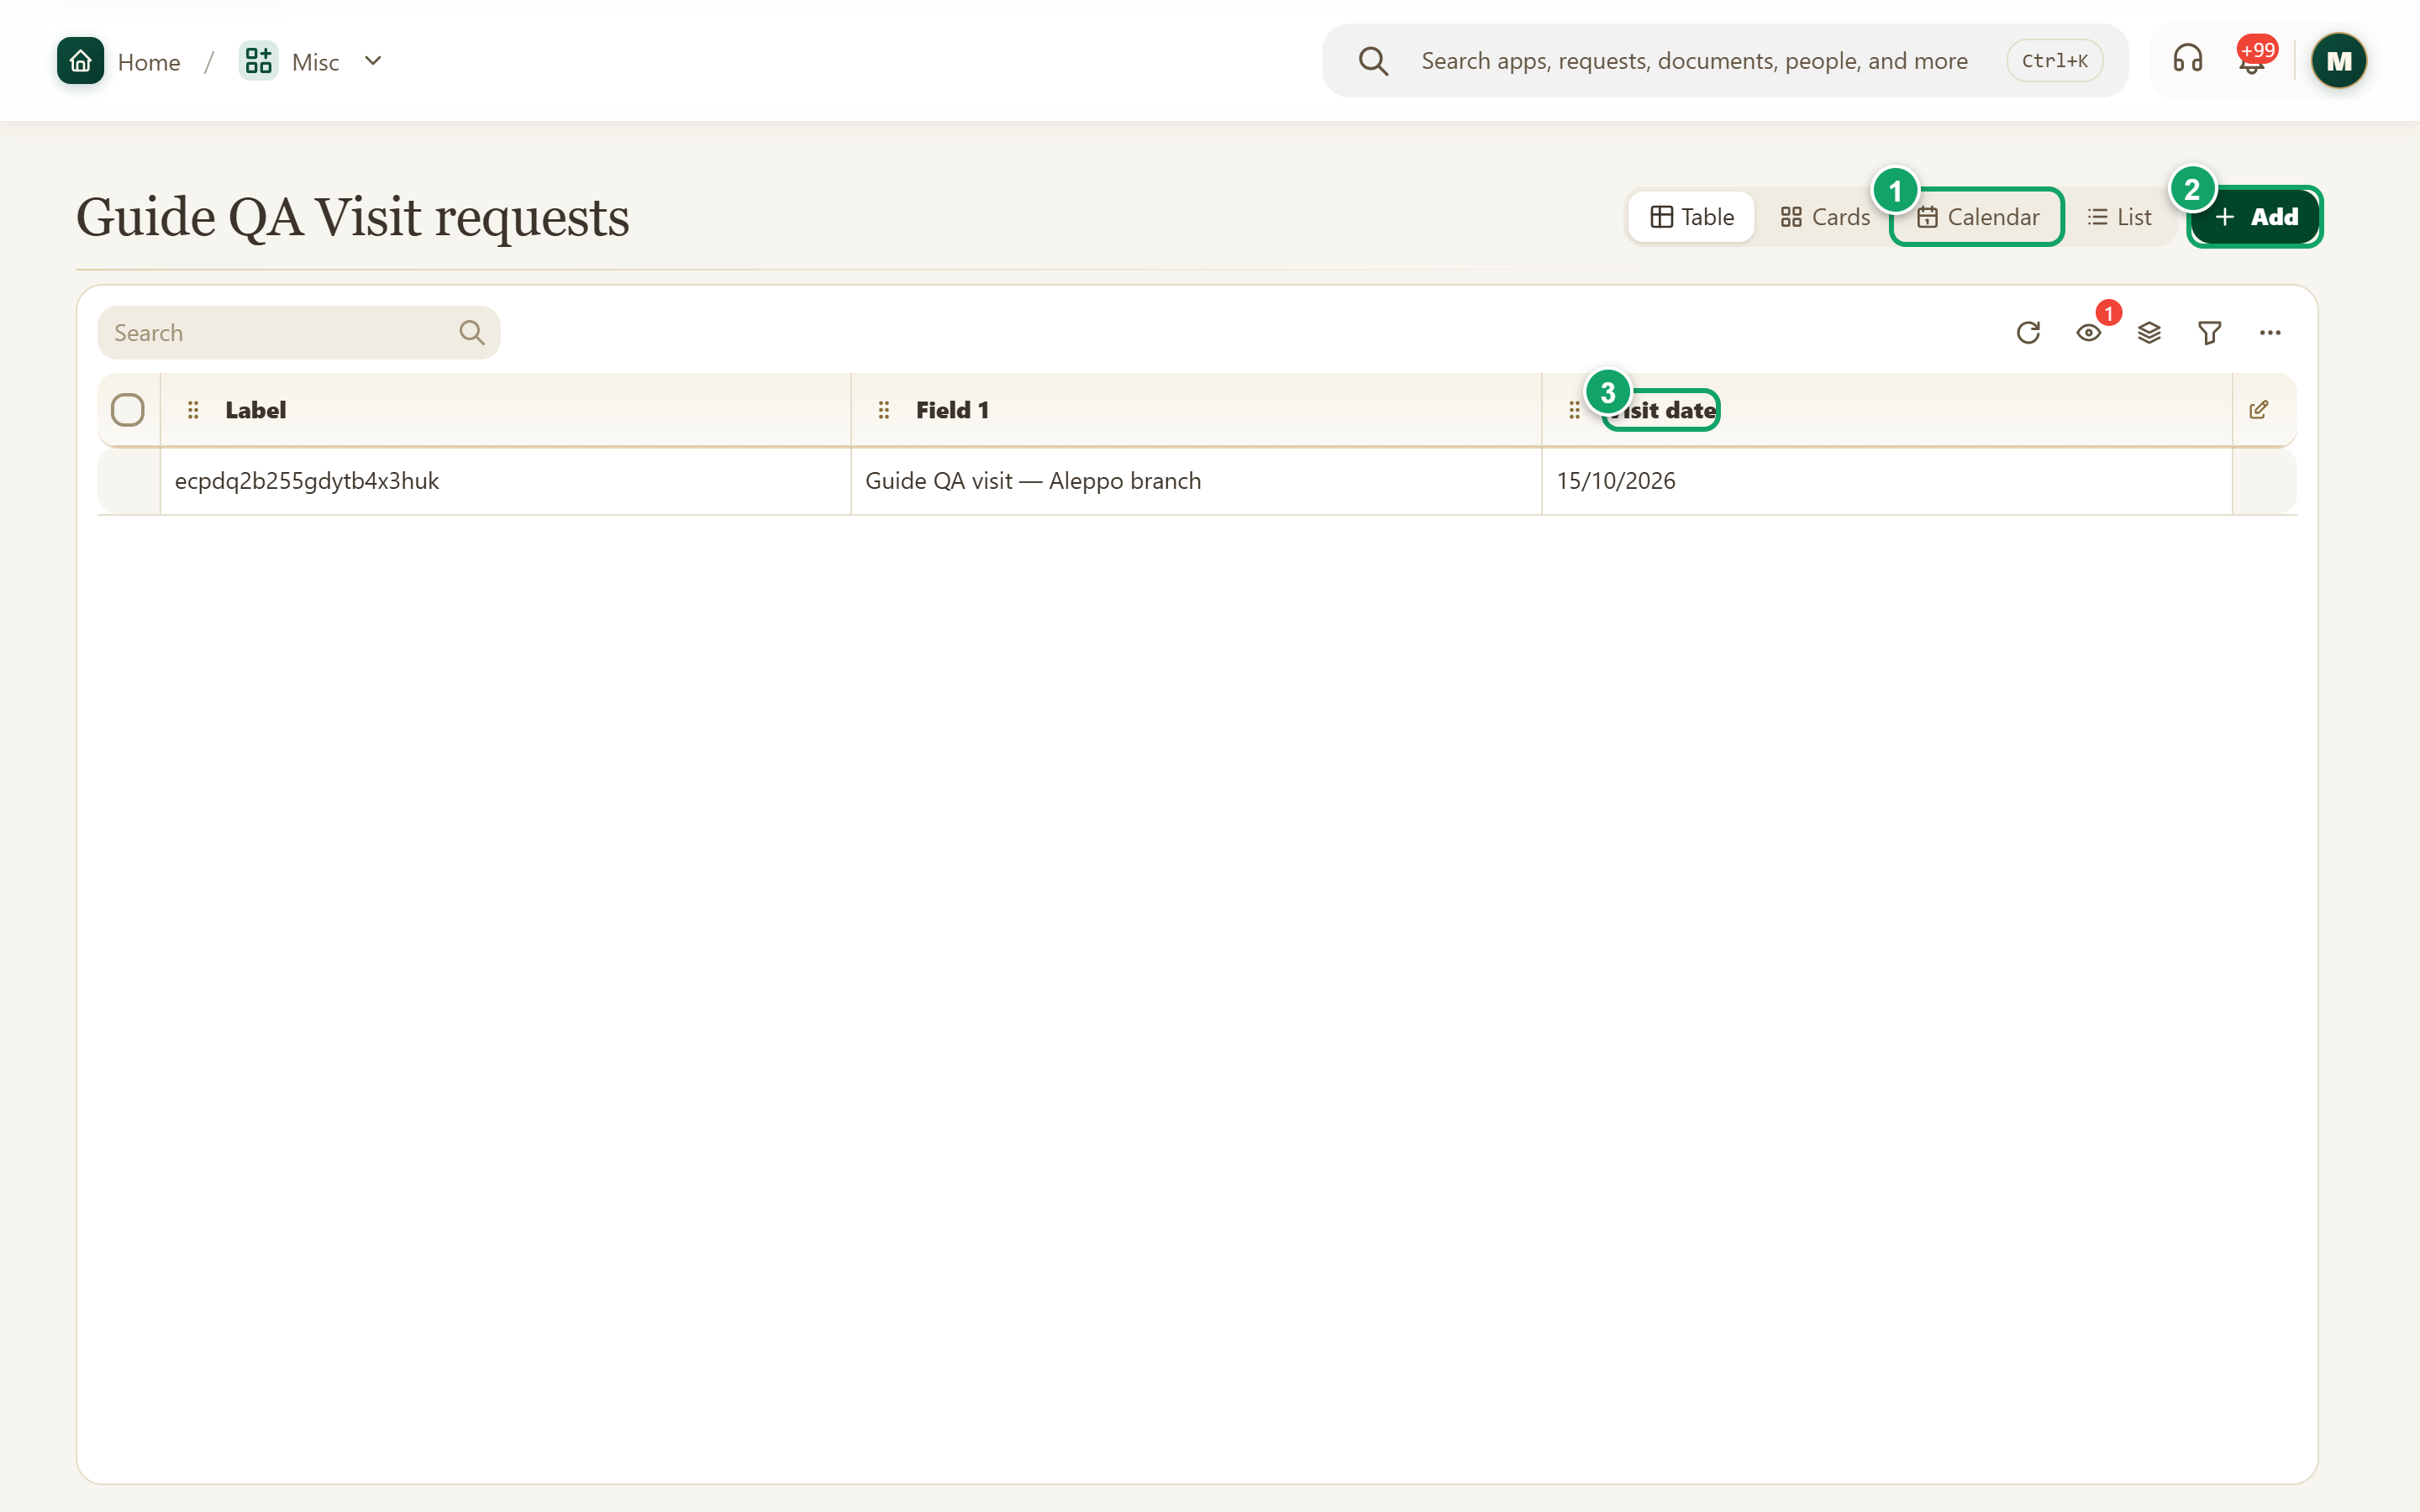
\includegraphics[width=0.95\linewidth,height=0.72\textheight,keepaspectratio]{figures/screens/ch06-records-en.png}
\caption{The type’s record list after publishing}
\label{fig:builder-lists-records}
\shotnote{This is the list users see after publishing, with a test record created on test2 and reopened to confirm it saved. ① “Calendar”: this view appeared because the type has a date field. ② “Add”. ③ The “Visit date” column: shows the test record’s saved value after it was reopened.}
\end{figure}


\begin{table}[H]
\centering
\caption{Available views}
\label{tab:builder-lists-modes}
\begin{tabularx}{\linewidth}{R{3.6cm} Y}
\rcHeaderRow
\thh{View} & \thh{When it fits}\\
Table and List & Always available for reviewing and comparing records row by row, with sorting and filtering.\\
Cards and Gallery & “Cards” is always available; “Gallery” appears when the type has a “File” field to show images from.\\
Kanban & Spreads records into columns by status or a select value, and appears when a suitable field exists.\\
Calendar and Timeline & Appear when the type has a date or time-range field, such as appointments and stages.\\
Map & Appears when the type has a “Location” or “Boundary” field.\\
Tree & Appears when you turn on “Parent records” in “Advanced”, showing records as parents and children.\\
\end{tabularx}
\end{table}

\begin{figure}[H]
\centering
\begin{tikzpicture}[node distance=0.5cm]
\node[entity] (fields) {Fields};
\node[entityOpt,below right=0.7cm and 0.3cm of fields] (cal) {Calendar};
\node[entityOpt,below left=0.7cm and 0.3cm of fields] (map) {Map};
\draw[dependsOnOpt] (fields.south) -- ++(0,-0.3) -| (cal.north);
\draw[dependsOnOpt] (fields.south) -- ++(0,-0.3) -| (map.north);
\end{tikzpicture}
\rclegend
\caption{Views that depend on the field type}
\label{fig:builder-lists-depends}
\shotnote{The figure shows that some views need a field of a certain type: the calendar needs a date, and the map needs a location or boundary. So if a view you want is missing, check the fields first, because the view does not appear among the options without the field it relies on.}
\end{figure}

\subsection{Steps and check}
\begin{enumerate}
\item Open the record type and choose “Lists \& views”.
\item Turn on the views the team needs, and choose the default view that opens first.
\item Choose the visible columns, order them by importance for daily work, and add summary figures when needed.
\end{enumerate}

\textbf{Check and recovery:} “Overview” should show the default view and the number of saved views. After publishing, open the record list and switch between views to confirm them; if a view is empty, check that the records have a value in the field it relies on.

\clearpage
\section{Figures and saved views}
\label{sec:builder-feature-figures-views}

These two tools help the team understand a list without opening every record. “Figures” are summary numbers above the list, such as the number of open requests or a total amount, and clicking a figure filters the list. “Saved views” are tabs above the list, each with ready filters, sorting and grouping, so users switch between “My requests” and “Waiting for review” in one click.

\textbf{Path and who uses it:} Builder workspace → “Lists \& views” → the “Figures” card and the “Saved views” card. The person who builds the type sets them, and everyone who opens the list sees them. Each user can also save views of their own from the list itself.

\begin{rcnote}[Example: Horizon]
Above the “Visit requests” list, the administrator adds a figure with the number of requests “Under review” that turns warning-coloured above five, and a saved view called “Waiting for my review” that shows Sarah Al-Khatib the requests waiting for her.
\end{rcnote}

\begin{figure}[H]
\centering
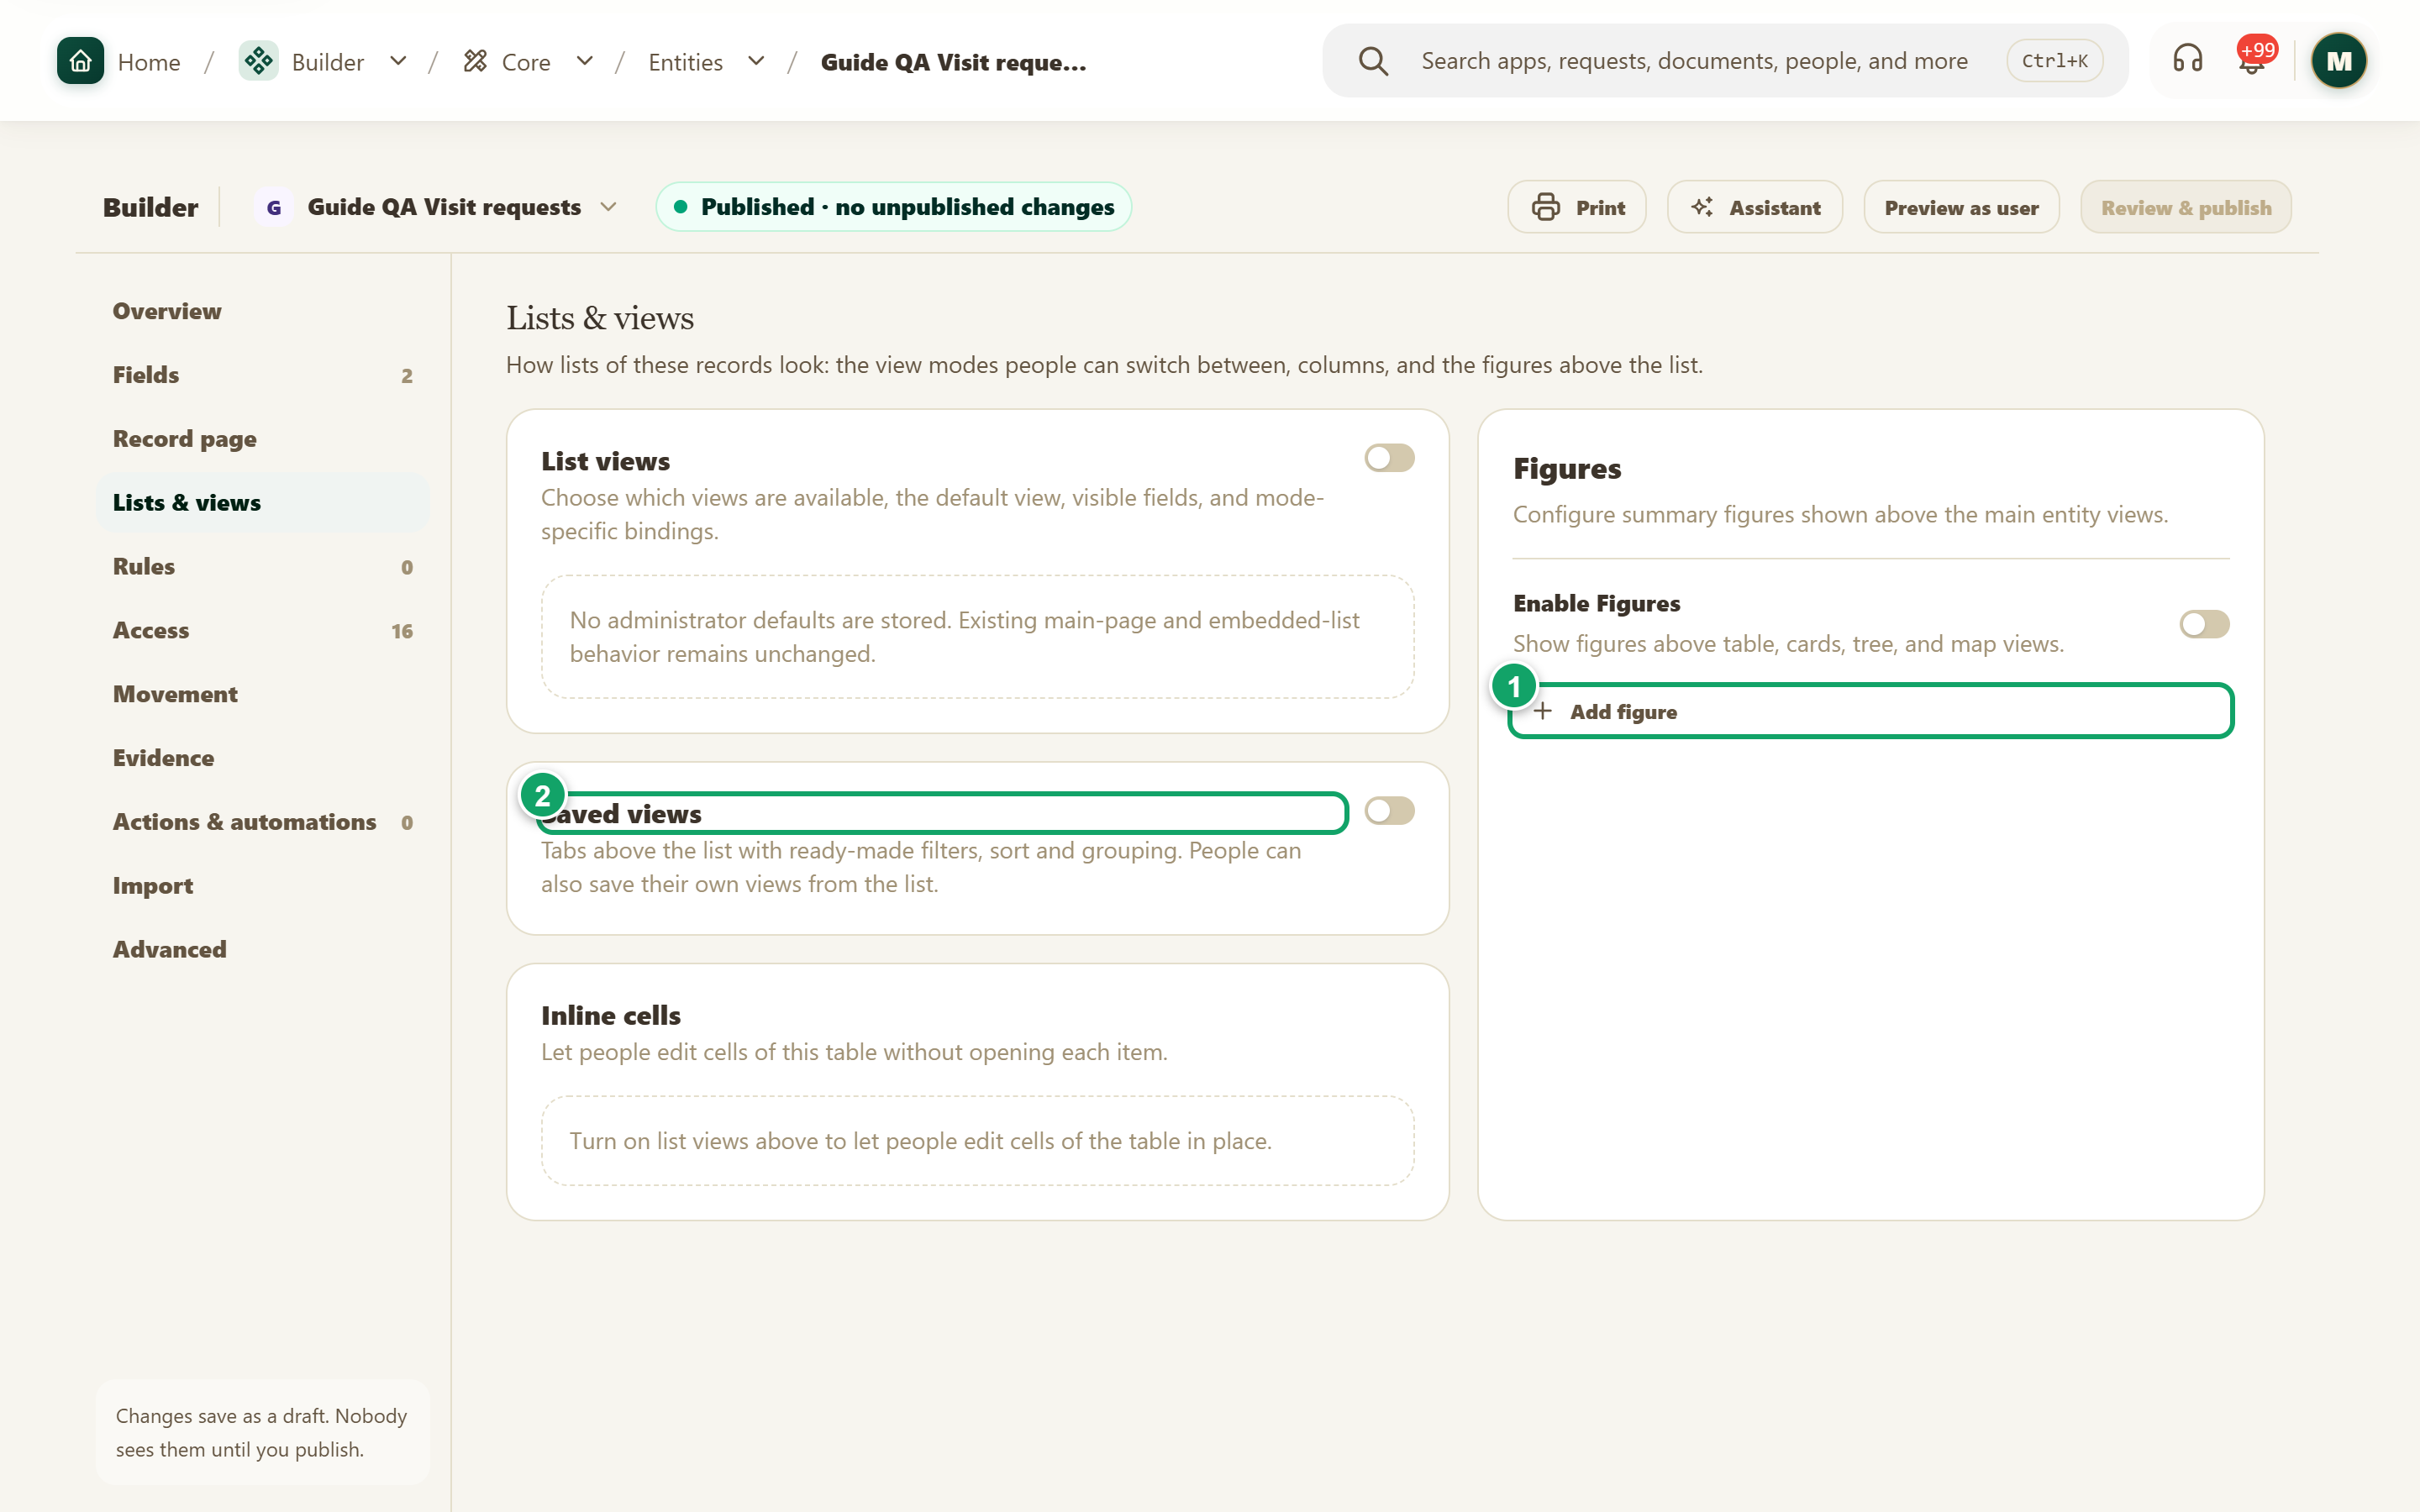
\includegraphics[width=0.95\linewidth,height=0.72\textheight,keepaspectratio]{figures/screens/ch06-ws-figures-views-en.png}
\caption{The figures and saved views cards in “Lists \& views”}
\label{fig:builder-figures-views-screen}
\shotnote{The image shows the “Lists \& views” section of the test type, with no figure or saved view added yet. It shows where to start when you want to summarize or organize the list. ① “Add figure”: adds a summary number above the list. ② “Saved views”: the card where you add ready tabs above the list.}
\end{figure}

\begin{table}[H]
\centering
\caption{Figure settings}
\label{tab:builder-figures-settings}
\begin{tabularx}{\linewidth}{R{3.6cm} Y}
\rcHeaderRow
\thh{Setting} & \thh{Meaning}\\
Figure type & “Single value”, “Ratio (part of a total)” shown with a bar, or “Distribution by status”.\\
Aggregation & Count, sum, average, minimum, maximum or weighted average of a numeric field.\\
Records counted & Records of this type or of a related type, with filters and a date window, such as the last thirty days.\\
Line under the figure & None, text, a second value, or the next upcoming record.\\
Highlight & Colours the figure “Warning” or “Critical” when the value is below or above a threshold.\\
\end{tabularx}
\end{table}

\begin{table}[H]
\centering
\caption{What a saved view keeps}
\label{tab:builder-saved-views-settings}
\begin{tabularx}{\linewidth}{R{3.6cm} Y}
\rcHeaderRow
\thh{Setting} & \thh{Meaning}\\
Name and colour & The tab's name and colour above the list; it can also show the record count.\\
Opens in & The view mode the tab opens in, or keeping the current view mode.\\
Sort and group & The field records are sorted by and the order, and the field they are grouped by.\\
Filters & The conditions that decide which records show; they can follow the viewer, such as “Me” or a number of days from today.\\
Records the viewer can act on & Shows only records on which the viewer can make a transition of the status field.\\
\end{tabularx}
\end{table}

\begin{figure}[H]
\centering
\begin{tikzpicture}[node distance=0.5cm]
\node[stepBox] (a) {Enable Figures};
\node[stepBox,below=of a] (b) {Add and set a figure};
\node[stepBox,below=of b] (c) {Add a saved view};
\node[stepBox,below=of c] (d) {Review and publish};
\node[stepBox,below=of d] (e) {Try it on the list};
\draw[flowsTo] (a) -- (b);
\draw[flowsTo] (b) -- (c);
\draw[flowsTo] (c) -- (d);
\draw[flowsTo] (d) -- (e);
\end{tikzpicture}
\rclegend
\caption{Summarizing and organizing a list}
\label{fig:builder-figures-views-flow}
\shotnote{The diagram puts both tools on one path because they work above the same list: a figure summarizes and a saved view filters. It ends by trying them on the list after publishing, because clicking a figure and switching tabs only show there.}
\end{figure}

\subsection{Steps and check}
\begin{enumerate}
\item Open “Lists \& views”, turn on “Enable Figures”, then press “Add figure”.
\item Choose the figure type, the aggregation and the field, add filters and a date window, then set the highlight if you need a visual alert.
\item In “Saved views”, turn on showing the tabs, press “Add view”, and write its name, filters and sorting.
\item Publish the changes, then open the list and click the figure and the new tab.
\end{enumerate}

\textbf{Check and recovery:} the figure should show above the list and filter it when clicked, and the tab should show the records matching its filters. If the figure does not show, make sure “Enable Figures” is on and the figure is not hidden. Remember that views added here are seen by everyone, while “Save view” on the list keeps a view only you see.

\clearpage
\section{Rules}
\label{sec:builder-feature-rules}

A rule makes a record behave according to its values, without the user having to remember it. It can show a field when a certain value is chosen, lock it after creation, make it required in a given situation, or refuse an illogical value. The “Rules” section gathers all of these rules in one list.

\textbf{Path and who uses it:} record type → “Rules”. Used by whoever builds the type, once the fields are complete.

\begin{rcnote}[Example: Horizon]
The system administrator adds a rule that shows the “Rejection reason” field only when the status is “Rejected”, and a rule that checks the visit date is on or after the request date. They add both rules from ①.
\end{rcnote}

\begin{figure}[H]
\centering
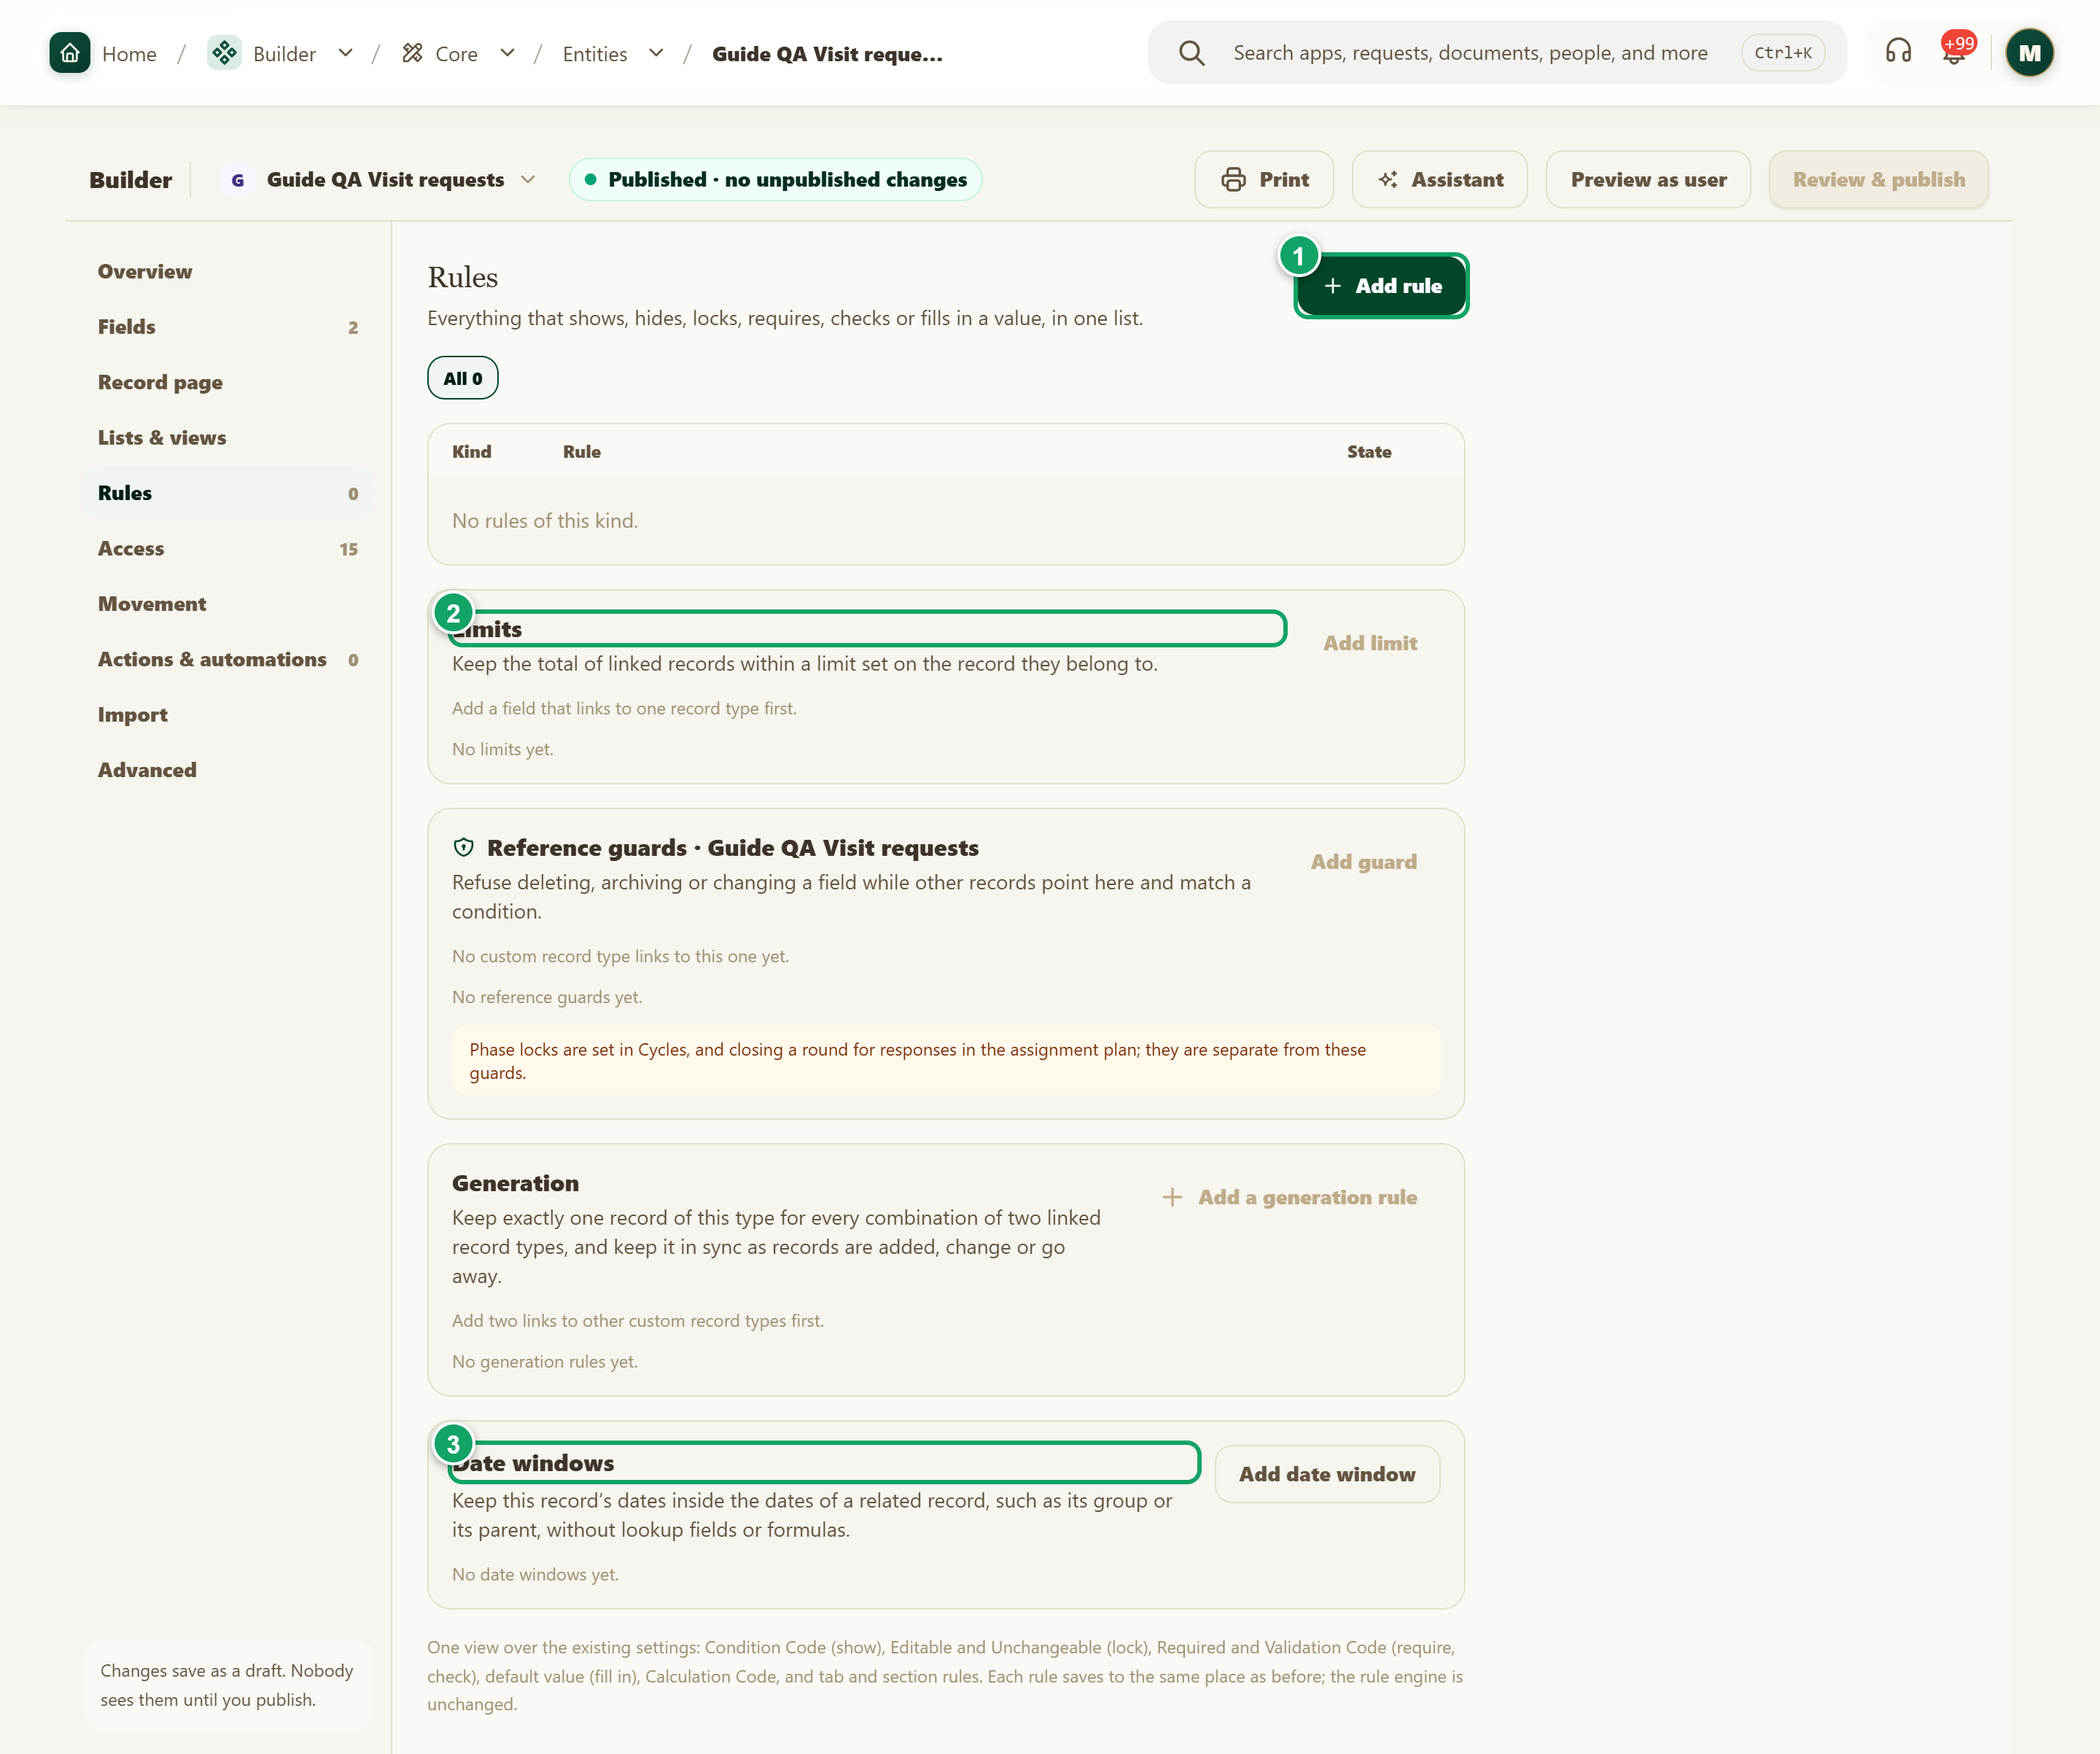
\includegraphics[width=0.95\linewidth,height=0.72\textheight,keepaspectratio]{figures/screens/ch06-ws-rules-en.png}
\caption{The “Rules” section and its extra tools}
\label{fig:builder-rules-screen}
\shotnote{The rules list sits at the top of the section, with other data-protecting tools below it, such as limits and date windows. The list is empty because the test type has no rules. ① “Add rule”. ② “Limits”: keeps the total of linked records within a limit. ③ “Date windows”: keeps the record’s dates inside a related record’s dates.}
\end{figure}


\begin{table}[H]
\centering
\caption{Rule kinds}
\label{tab:builder-rules-kinds}
\begin{tabularx}{\linewidth}{R{3.6cm} Y}
\rcHeaderRow
\thh{Kind} & \thh{What does it do?}\\
Show or hide & Shows a field, tab or section when a condition is met and hides it otherwise.\\
Lock editing & Prevents changes to a field, tab or section: “Locked when” a condition is met, “Editable only when”, or “After creation”.\\
Require & Makes the field required “Always” or “Only when…” a condition is met, with a message explaining why.\\
Check value & Refuses the value unless it is, for example, more than a number, after a date or different from another field, and shows your message.\\
Fill in value & Starts the field with a ready value the user can change.\\
Calculate & Lists calculated fields; you edit them in the “Fields” section.\\
\end{tabularx}
\end{table}

\begin{table}[H]
\centering
\caption{Other rules that live elsewhere}
\label{tab:builder-rules-other}
\begin{tabularx}{\linewidth}{R{3.6cm} Y}
\rcHeaderRow
\thh{Rule} & \thh{Where do you find it?}\\
Limits & Under the rules list: keeps the total or count of linked records within a limit, then refuses the excess or warns and asks for a reason.\\
Lifecycle rules & On the “Status” field in “Fields”: for each status you decide whether the record is “Locked” or “Locked except…”, and you can “Block delete”. Needs a fixed status template.\\
Unique values & In “Advanced”: prevents two records from sharing a code or a combination of values.\\
\end{tabularx}
\end{table}

\begin{figure}[H]
\centering
\begin{tikzpicture}[node distance=0.5cm]
\node[stepBox] (a) {Choose the rule kind};
\node[stepBox,below=of a] (b) {Condition: When…};
\node[stepBox,below=of b] (c) {Target: field, tab or section};
\node[stepBox,below=of c] (d) {Try it, then save to draft};
\draw[flowsTo] (a) -- (b);
\draw[flowsTo] (b) -- (c);
\draw[flowsTo] (c) -- (d);
\end{tikzpicture}
\rclegend
\caption{How a rule is built}
\label{fig:builder-rules-flow}
\shotnote{A rule reads like a sentence: “When” a condition is met, apply an effect to a chosen target. The diagram puts the test before saving, because “Try it” runs the rule on sample records and exposes a wrong condition before it reaches users. Rules apply to everyone who can edit the record, so they are not a way to treat one role differently from another.}
\end{figure}

\subsection{Steps and check}
\begin{enumerate}
\item Open the record type, choose “Rules”, then press “Add rule”.
\item Choose the rule kind, then build the condition under “When”, joining conditions with “+ And” or “+ Or”.
\item Pick the target from “Choose a field, tab or section”, and write the “Message people see” when needed.
\item Press “Try it” and review the result on the samples, then press “Save to draft”.
\end{enumerate}

\textbf{Check and recovery:} the rule should appear in the table with the state “OK”. If it shows “Broken”, open it and fix the field or condition that changed. If you want only some roles to see a field, use “Access”, not “Rules”.

\clearpage
\section{Limits, reference guards, generation and date windows}
\label{sec:builder-feature-record-limits}

These four tools sit below the rules table in the “Rules” section and protect data from mistakes that are hard to find later. “Limits” prevent the total of linked records from exceeding a limit, “Reference guards” prevent deleting or changing a record while other records depend on it, “Generation” keeps one record for every combination of two linked types, and “Date windows” keep a record's dates inside the dates of a related record.

\textbf{Path and who uses it:} Builder workspace → “Rules”, then at the bottom of the page: “Limits”, “Reference guards”, “Generation” and “Date windows”. Used by people who build financial and organizational types that need controls between records.

\begin{rcnote}[Example: Horizon]
The administrator adds a date window that keeps the visit date inside the dates of the visit plan linked to the request, and a guard that prevents deleting a branch while it has open visit requests.
\end{rcnote}

\begin{figure}[H]
\centering
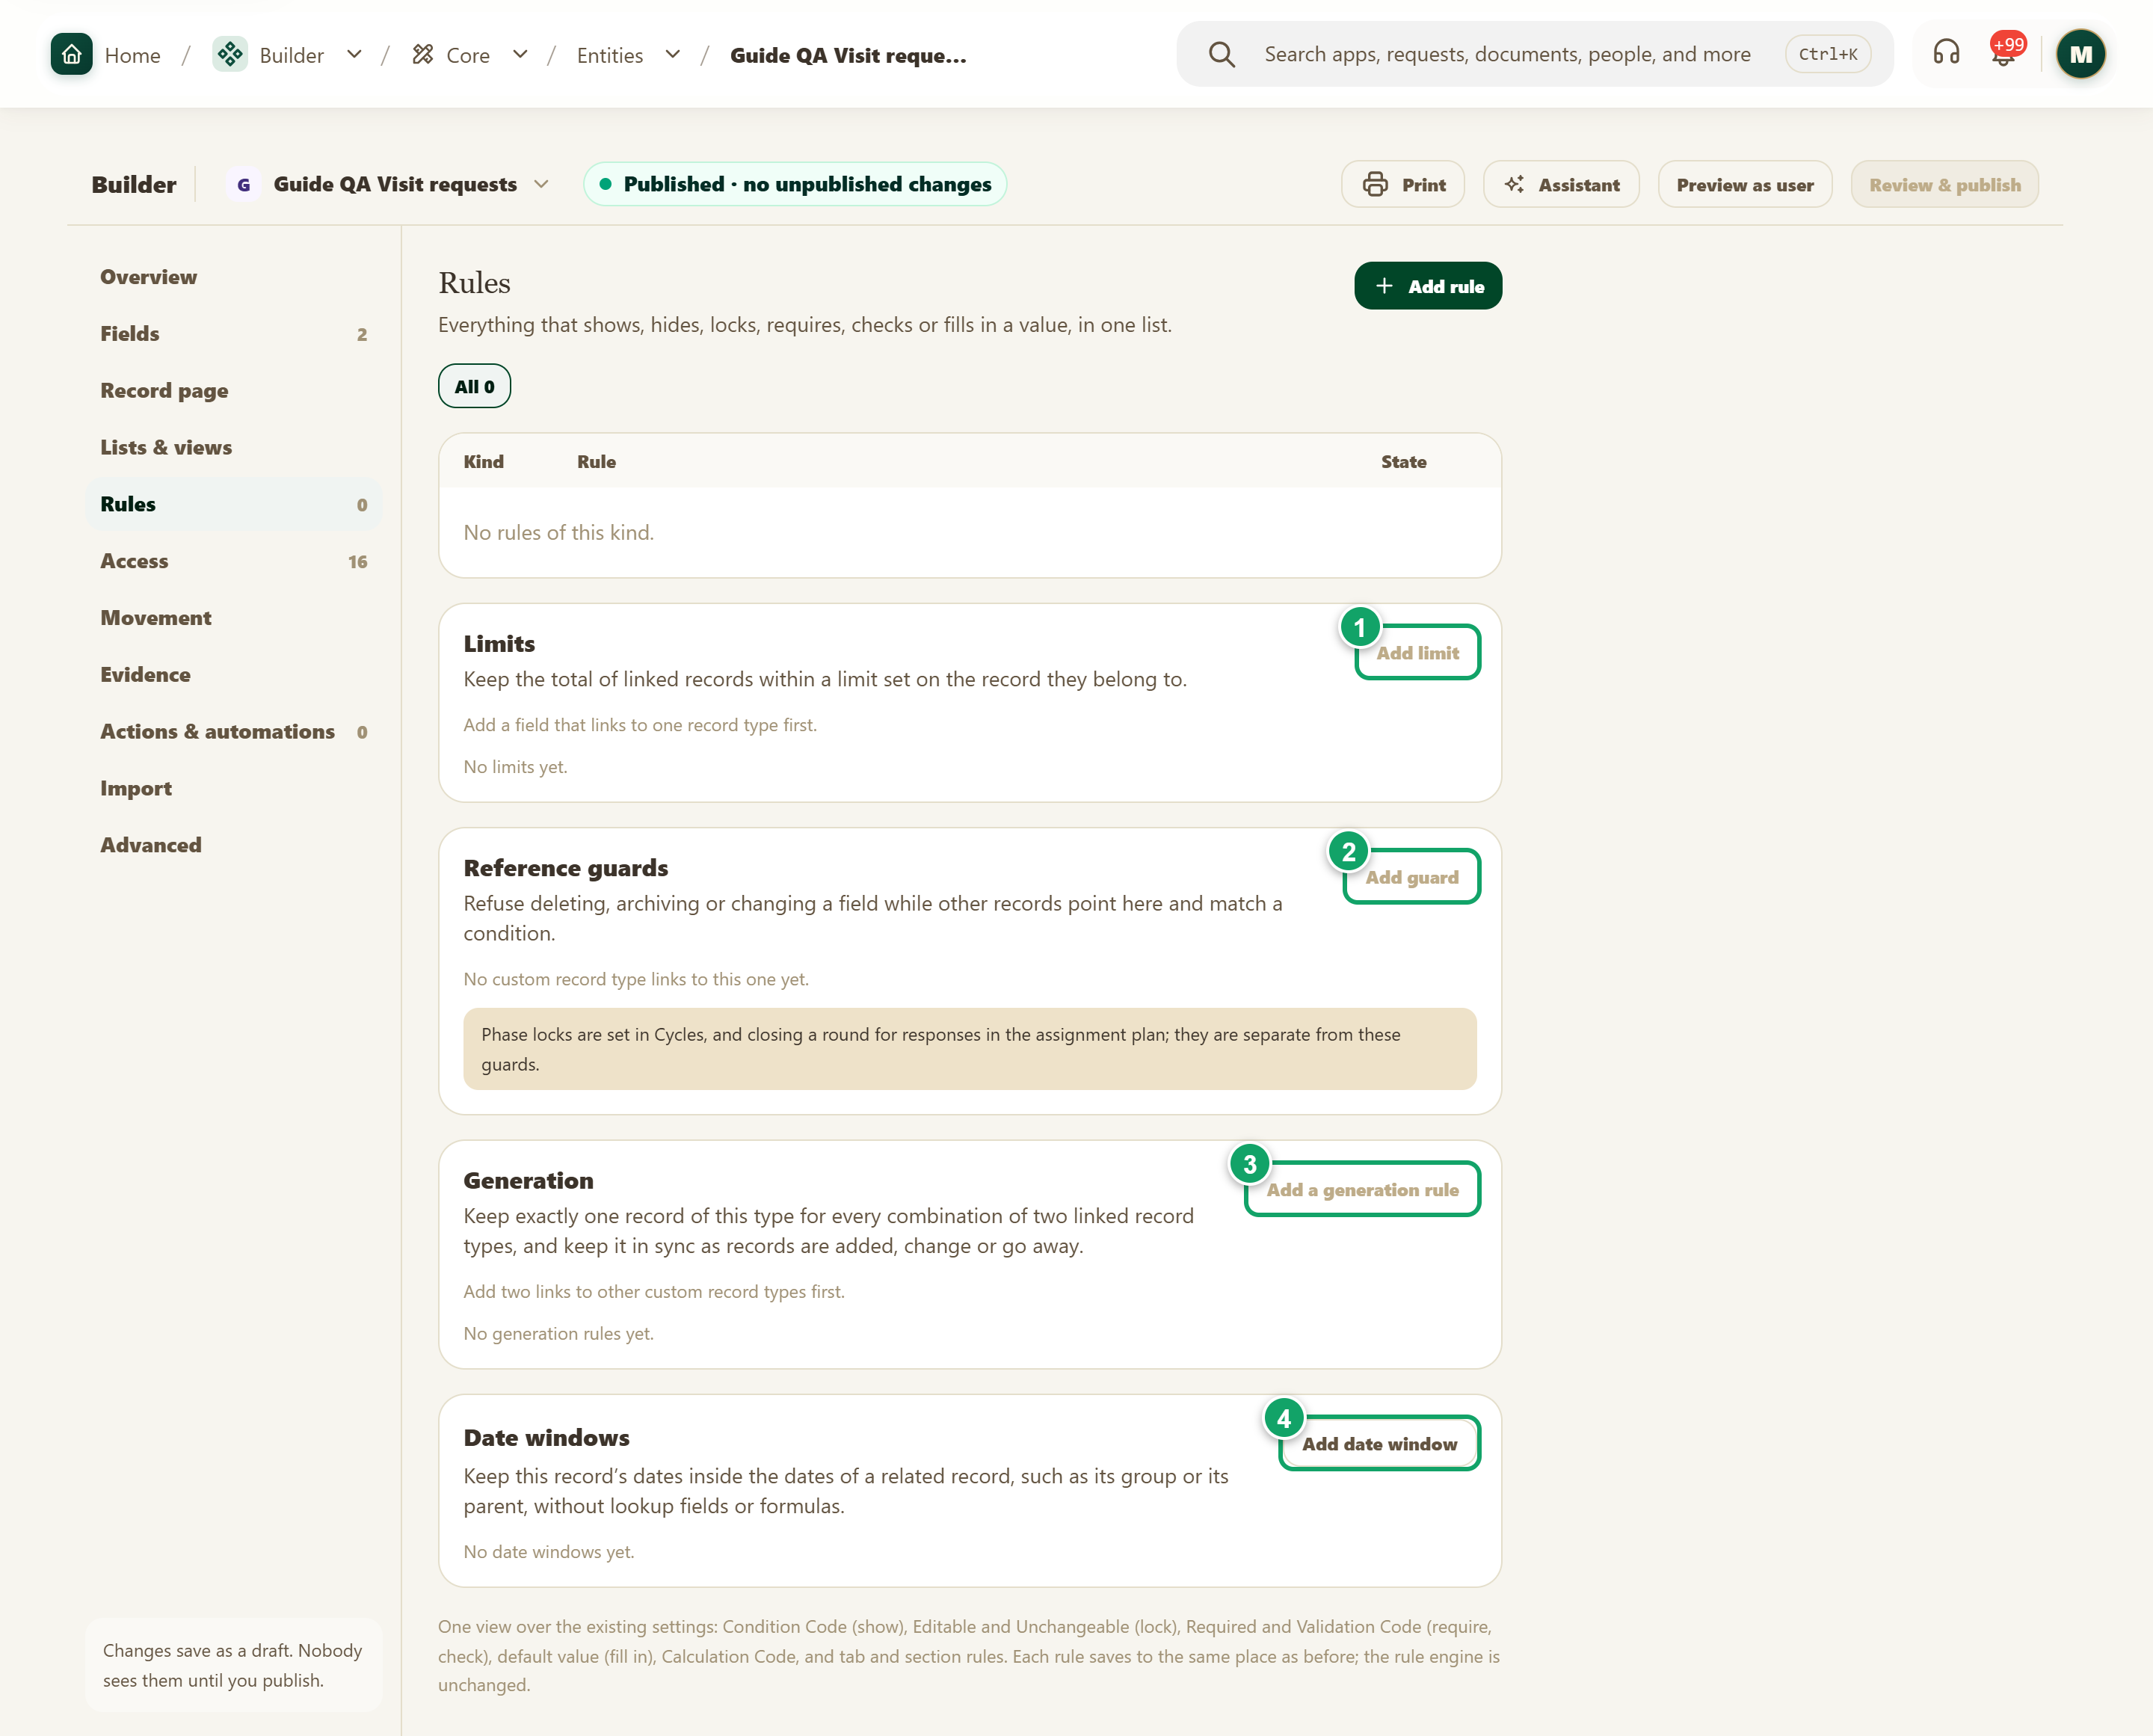
\includegraphics[width=0.95\linewidth,height=0.72\textheight,keepaspectratio]{figures/screens/ch06-ws-rule-tools-en.png}
\caption{The four tools below the rules table}
\label{fig:builder-record-limits-screen}
\shotnote{The image shows the “Rules” section of the test type, with a card for each tool below the rules table and its own add button. Each card shows what it needs before use, such as a relation field. ① “Add limit”. ② “Add guard”. ③ “Add a generation rule”. ④ “Add date window”. Each button starts an editor that leads you to complete the sentence describing the control.}
\end{figure}

\begin{table}[H]
\centering
\caption{The four tools}
\label{tab:builder-record-limits-tools}
\begin{tabularx}{\linewidth}{R{3.6cm} Y}
\rcHeaderRow
\thh{Tool} & \thh{What it does and what you set}\\
Limits & Keeps the total of linked records within a limit set on the record they belong to, such as spending lines within a budget. You set “What to add up”, “Across”, the “Limit”, and what happens “When over”: refuse, or warn and ask for a reason that goes to the deciding roles.\\
Reference guards & Refuse deleting, archiving or changing a field of the record while other records point to it and match a condition, with a message that explains why. A record type can have at most ten guards.\\
Generation & Keeps one record of this type for every combination of records of two linked types, and keeps it in sync when they change, such as one evaluation record per employee per cycle. “Preview” shows the counts, “Fill now” creates the missing ones, and it does not run before the type is published.\\
Date windows & Keep the start and end dates inside the dates of a related record or the parent, and decide what happens when those dates change: allow it and list the records left outside, or refuse the change. Users see a phrase such as “Between … and …” on the record.\\
\end{tabularx}
\end{table}

\begin{figure}[H]
\centering
\begin{tikzpicture}[node distance=0.5cm]
\node[stepBox] (a) {Name the risk to the data};
\node[stepBox,below=of a] (b) {Choose the matching tool};
\node[stepBox,below=of b] (c) {Set it and write its message};
\node[stepBox,below=of c] (d) {Preview or try it};
\node[stepBox,below=of d] (e) {Review and publish};
\draw[flowsTo] (a) -- (b);
\draw[flowsTo] (b) -- (c);
\draw[flowsTo] (c) -- (d);
\draw[flowsTo] (d) -- (e);
\end{tikzpicture}
\rclegend
\caption{Adding a control between records}
\label{fig:builder-record-limits-flow}
\shotnote{The diagram starts with the risk, not the tool, because each tool handles a different risk: an exceeded amount, a used record being deleted, missing records, or conflicting dates. Writing the message comes with the setup because a user whose change is refused needs a clear reason to know what to do.}
\end{figure}

\subsection{Steps and check}
\begin{enumerate}
\item Name the risk you want to prevent, then open “Rules” and scroll down to the matching tool.
\item Press the tool's add button, such as “Add limit”, and complete the sentence the editor shows step by step.
\item Write a message that tells the user why the change is refused and what they can do.
\item Use “Preview” where available, then publish the changes and try the forbidden case with a test record.
\end{enumerate}

\textbf{Check and recovery:} the forbidden change should be refused with your message, and a valid change accepted. If “Before you publish” says the settings of a limit, guard or generation rule are invalid, open them from the fix button and complete the missing field. Remember that generation needs the type to be published before it runs.

\clearpage
\section{Access}
\label{sec:builder-feature-access}

Access decides who can do what with the records of this type. These actions are called “verbs”, such as seeing records in lists, opening, adding, changing and deleting them. The “Access” section shows roles and verbs in one grid, and it edits the same roles as Settings › Roles, so it does not create a second permission system.

\textbf{Path and who uses it:} record type → “Access”. Used by whoever builds the type and holds the right to update roles.

\begin{rcnote}[Example: Horizon]
The system administrator gives branch coordinators, including Omar Haddad, the create and open verbs on “Visit requests”, and gives the HR Manager Sarah Al-Khatib the update verb so she can record her decision. Then they confirm Omar’s access with tool ③.
\end{rcnote}

\begin{figure}[H]
\centering
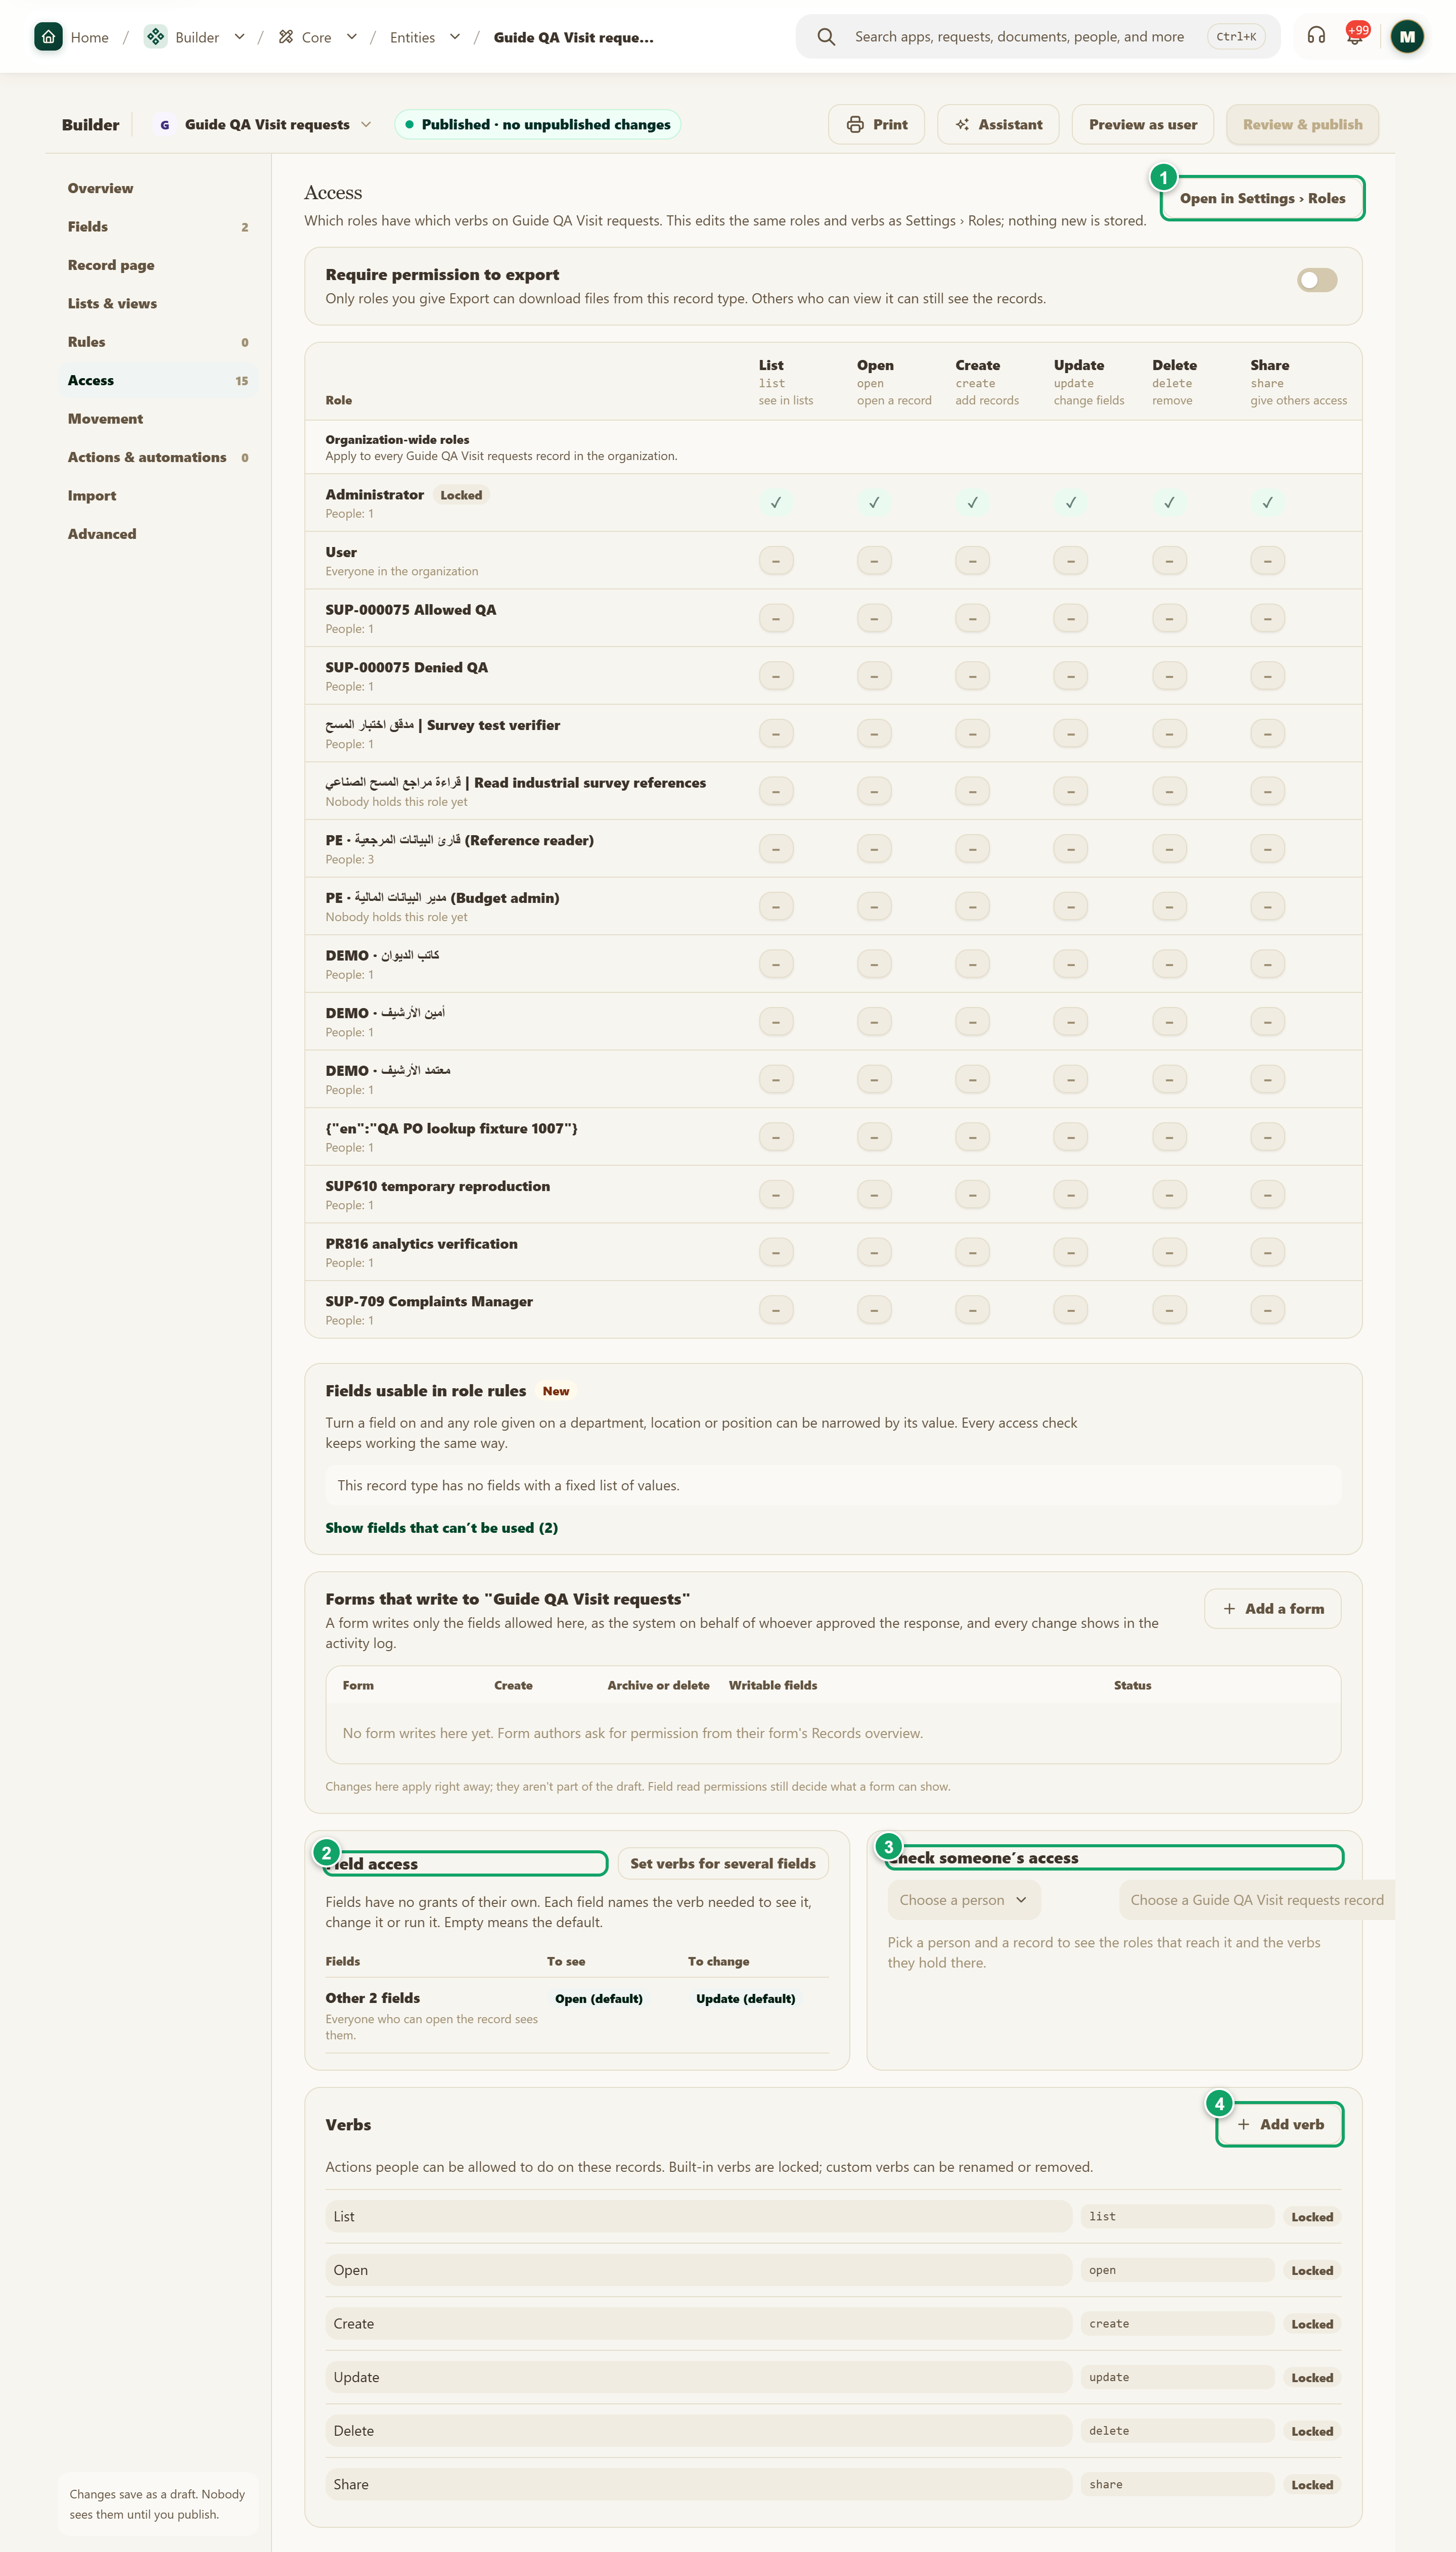
\includegraphics[width=0.95\linewidth,height=0.72\textheight,keepaspectratio]{figures/screens/ch06-ws-access-en.png}
\caption{The “Access” section}
\label{fig:builder-access-screen}
\shotnote{The section shows roles and verbs on this type, then field access, an access check tool and the verbs list. The roles shown are the test organization’s roles. ① “Open in Settings › Roles”. ② “Field access”: sets the verb needed to see or change a field. ③ “Check someone’s access”: shows what a person can do on a record. ④ “Add verb”: adds a custom verb such as approval.}
\end{figure}


\begin{table}[H]
\centering
\caption{Built-in verbs}
\label{tab:builder-access-verbs}
\begin{tabularx}{\linewidth}{R{3.6cm} Y}
\rcHeaderRow
\thh{Verb} & \thh{What does it allow?}\\
\en{list} & See in lists.\\
\en{open} & Open a record.\\
\en{create} & Add records.\\
\en{update} & Change fields.\\
\en{delete} & Remove.\\
\en{share} & Give others access.\\
\en{export} & Download a file; it appears when “Require permission to export” is on.\\
\end{tabularx}
\end{table}

\begin{table}[H]
\centering
\caption{What do you find here?}
\label{tab:builder-access-data}
\begin{tabularx}{\linewidth}{R{3.6cm} Y}
\rcHeaderRow
\thh{Card} & \thh{Content and action}\\
Roles and verbs & Press a cell to grant a verb to a role or take it away. It shows organization-wide roles, roles on one record, and other roles with grants here.\\
Field access & Fields have no grants of their own; each field names the verb needed “To see”, “To change” or “To run” it. Empty means the default.\\
Verbs & “Add verb” for a custom verb, such as “Approve budget”, then grant it to roles.\\
Fields usable in role rules & Let a role be narrowed by a field's value, such as the branch.\\
Require permission to export & When on, only roles holding the \en{export} verb can download files from this type; people who can view the records still see them.\\
Forms that write to this type & Decides which forms may write this type's fields. Changes here apply right away; they are not part of the draft.\\
Check someone’s access & Pick a person and a record to see the roles that reach it and the verbs they hold.\\
\end{tabularx}
\end{table}

\begin{figure}[H]
\centering
\begin{tikzpicture}[node distance=0.5cm]
\node[entity] (role) {Role};
\node[entity,below=0.7cm of role] (verb) {Verb};
\node[entityOpt,below right=0.7cm and 0.3cm of verb] (field) {Field that needs the verb};
\node[entityOpt,below left=0.7cm and 0.3cm of verb] (records) {Records of the type};
\draw[dependsOn] (role) -- (verb);
\draw[dependsOnOpt] (verb.south) -- ++(0,-0.3) -| (field.north);
\draw[dependsOnOpt] (verb.south) -- ++(0,-0.3) -| (records.north);
\end{tikzpicture}
\rclegend
\caption{From role to what a person can do}
\label{fig:builder-access-model}
\shotnote{The figure shows that a person does not receive a permission directly but through their role, and the role holds verbs on the type's records. A sensitive field can ask for a specific verb, so only those holding it can see or change it. Start with the built-in verbs, and add a custom verb only for work that has its own meaning, such as approval.}
\end{figure}

\subsection{Steps and check}
\begin{enumerate}
\item Open the record type, choose “Access”, and review the roles shown.
\item Press the cells to give each role only the verbs its work needs.
\item For sensitive fields, open “Field access” and set the verb needed to see or change them.
\item Use “Check someone’s access” on an employee and a test record, then publish the changes.
\end{enumerate}

\textbf{Check and recovery:} the check tool should show the expected verbs for the person, and after publishing the user should see only what concerns them. If the message “You need the Update verb on roles to change grants.” appears, ask the organization administrator; if a field does not appear for a user, review the verb it needs under “Field access”.

\clearpage
\section{Field access and checking someone's access}
\label{sec:builder-feature-field-access}

The type's access decides who sees and changes records, but some fields need finer protection, such as an amount field or the reviewer's notes. This page explains three cards in the “Access” section: “Field access”, which sets the verb needed to see and change each field; “Fields usable in role rules”, which narrows a role by a value in the record; and “Check someone's access”, which shows what a given person actually gets.

\textbf{Path and who uses it:} Builder workspace → “Access”. Used by the person who builds the type together with whoever manages roles, because the section edits the same roles and verbs as “Settings” → “Roles”.

\begin{rcnote}[Example: Horizon]
The administrator makes the “Review notes” field of “Visit requests” read-only except for those holding the approval verb, then uses “Check someone's access” with Omar Haddad and one of his requests to confirm that Omar sees the notes and cannot change them.
\end{rcnote}

\begin{figure}[H]
\centering
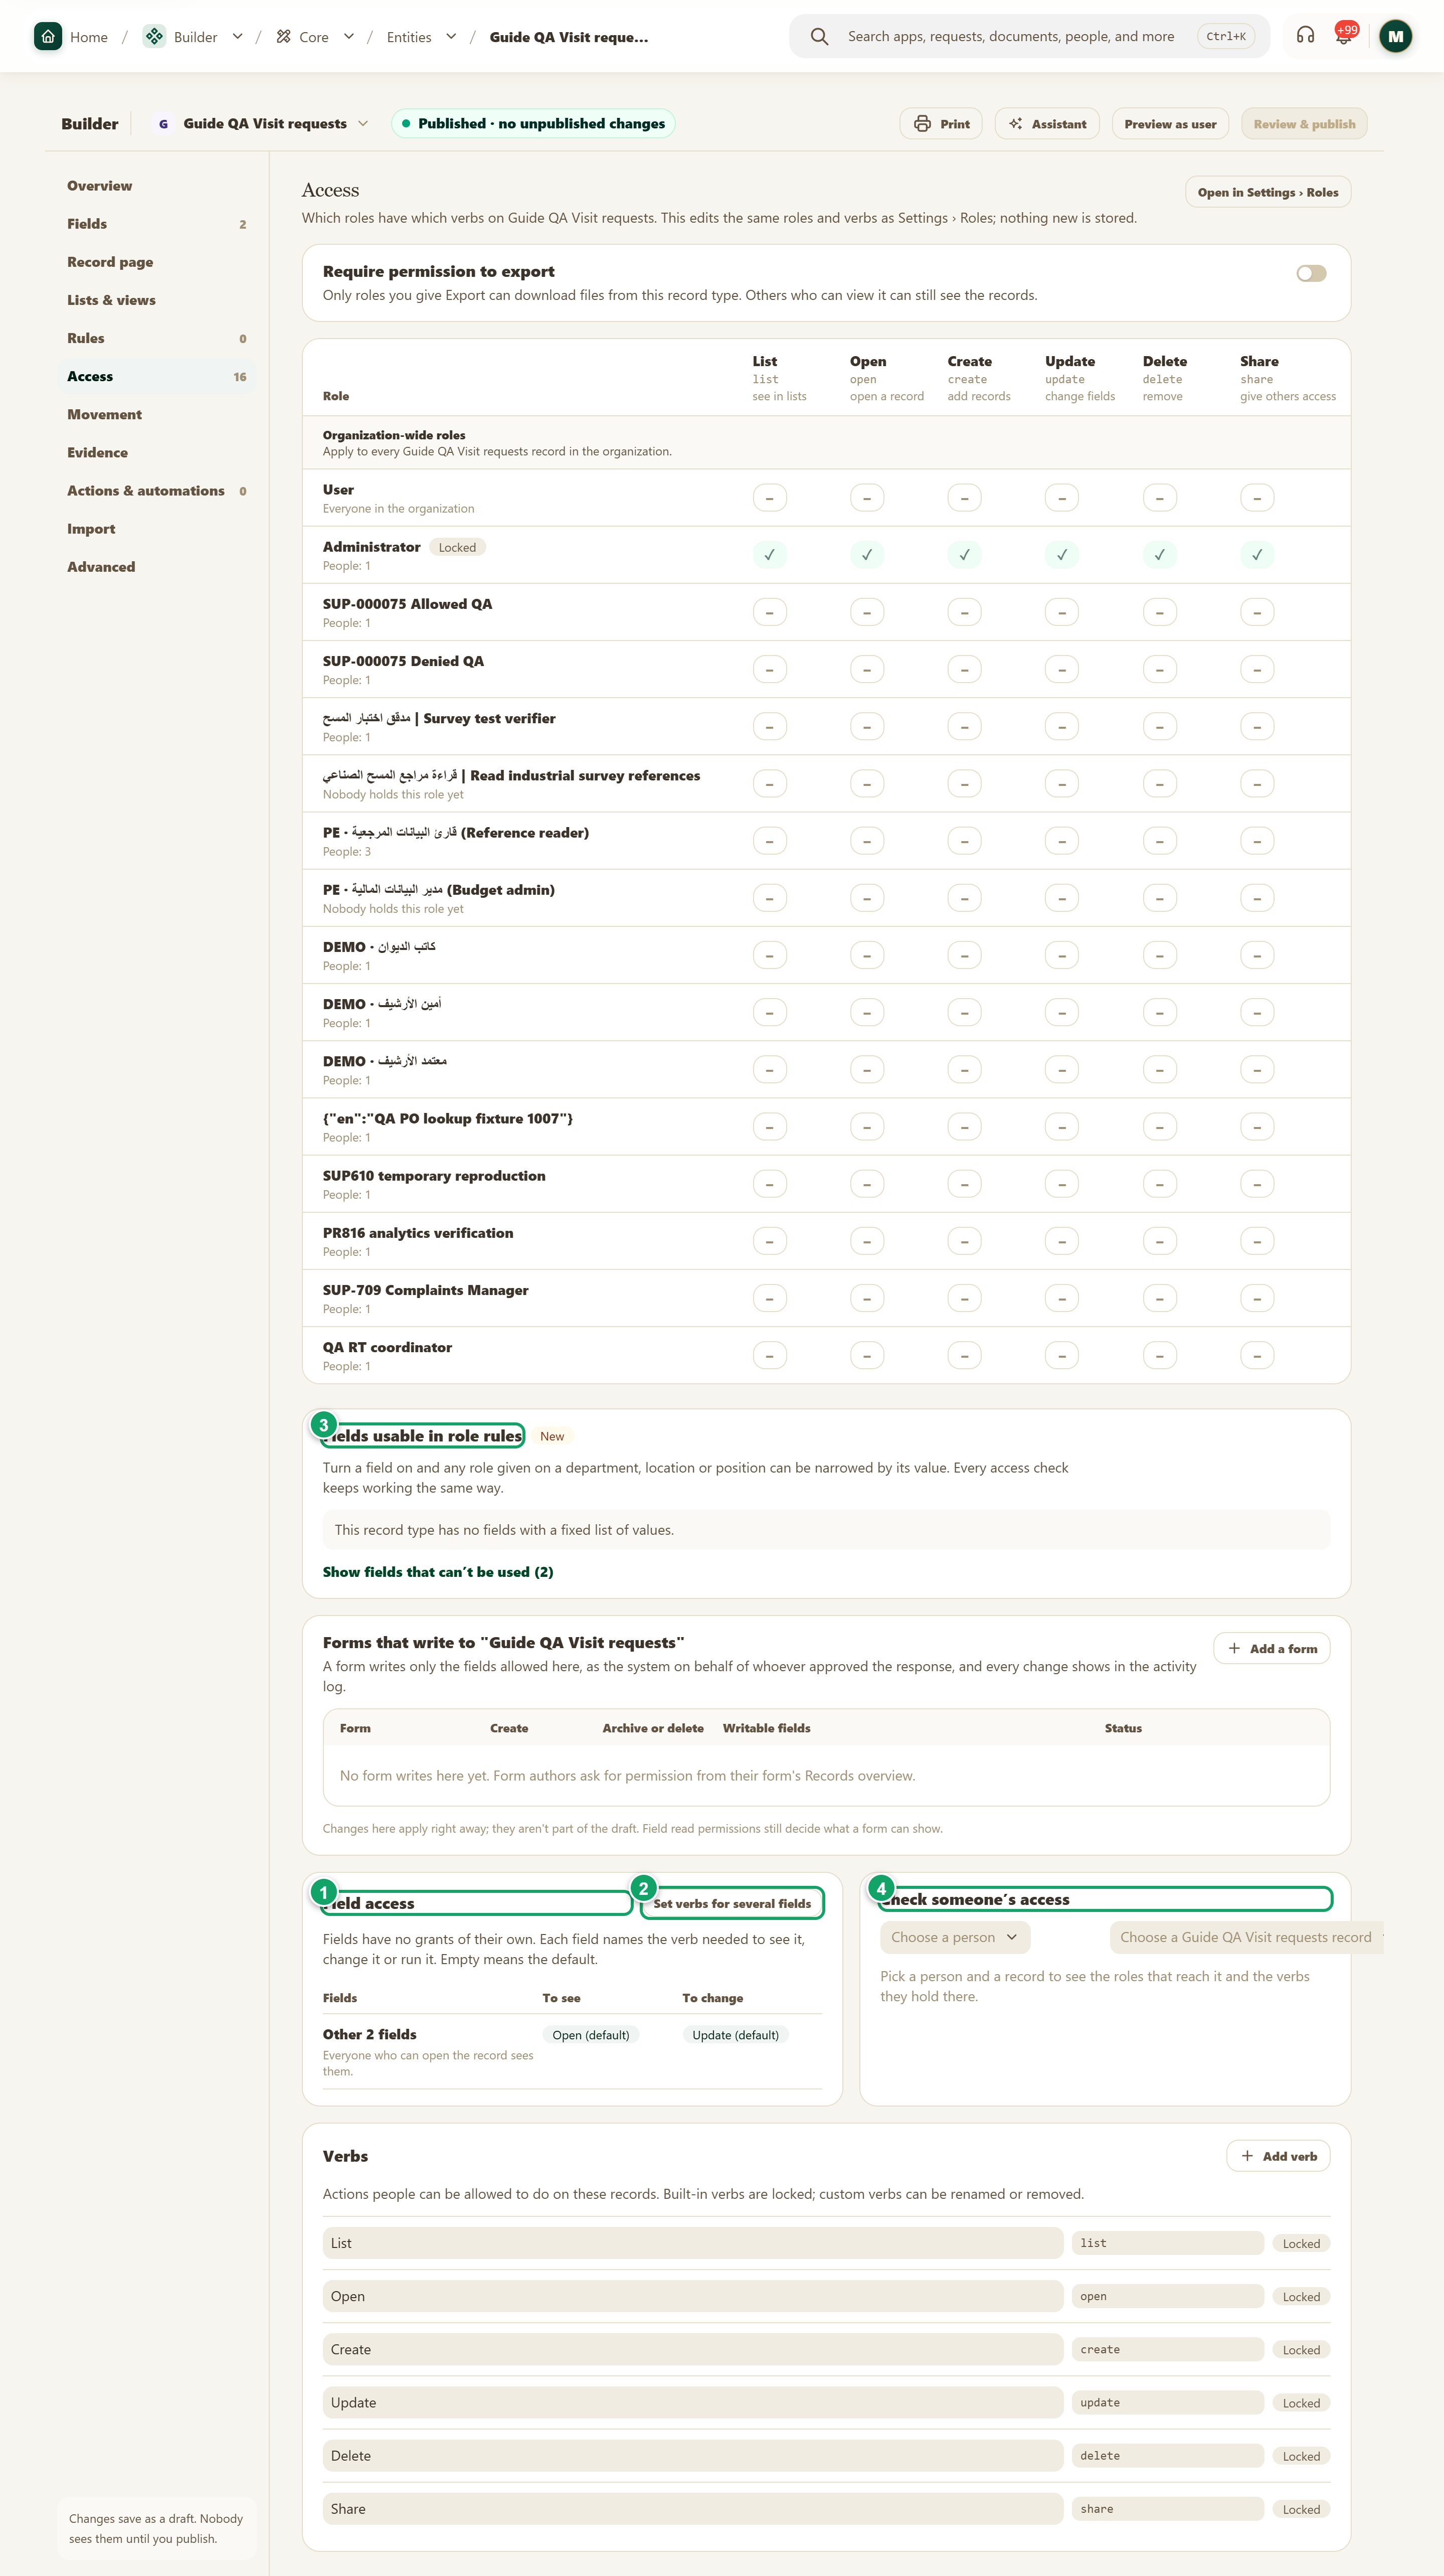
\includegraphics[width=0.95\linewidth,height=0.72\textheight,keepaspectratio]{figures/screens/ch06-ws-field-access-en.png}
\caption{The fine-grained access cards in the “Access” section}
\label{fig:builder-field-access-screen}
\shotnote{The image shows the whole “Access” section of the test type, including the cards that set field access and check what a given person gets. It helps you know their order on the page before you start. ① “Field access”: the table of verbs needed to see and change each field. ② “Set verbs for several fields”. ③ “Fields usable in role rules”: narrows a role by a value in the record. ④ “Check someone’s access”: checks what a person gets on a record.}
\end{figure}

\begin{table}[H]
\centering
\caption{The fine-grained access cards}
\label{tab:builder-field-access-cards}
\begin{tabularx}{\linewidth}{R{3.6cm} Y}
\rcHeaderRow
\thh{Card} & \thh{What it offers}\\
Field access & A table of fields with two columns for each: “To see” and “To change”. In each you choose the needed verb, or leave it empty to follow the record's default access. Each row shows who the field is hidden from and who sees it read-only.\\
Set verbs for several fields & You choose several fields and set “To see” and “To change” for them together: keep as it is, the default, a given verb, or the system only. Then press “Apply”, and the change goes to the draft.\\
Fields usable in role rules & You turn on a relation, dropdown or yes/no field, so a role given on a department, location or position can be narrowed by that field's value. Text, number, date and multi-value fields cannot be used, and a field roles already use is locked.\\
Check someone’s access & You choose a person and a record, and see the roles that reach the record, the verbs the person holds with those they lack struck through, and how many fields are hidden from them or read-only. The check uses the draft's access, so you can verify before publishing.\\
\end{tabularx}
\end{table}

\begin{figure}[H]
\centering
\begin{tikzpicture}[node distance=0.5cm]
\node[stepBox] (a) {Verbs on the type};
\node[stepBox,below=of a] (b) {Field access};
\node[stepBox,below=of b] (c) {Check someone's access};
\node[stepBox,below=of c] (d) {Review and publish};
\draw[flowsTo] (a) -- (b);
\draw[flowsTo] (b) -- (c);
\draw[flowsTo] (c) -- (d);
\end{tikzpicture}
\rclegend
\caption{Setting field access and confirming it}
\label{fig:builder-field-access-flow}
\shotnote{The diagram starts with the type's verbs because a field's access is written with one of them, so it means nothing before roles get their verbs. It places the check on a given person before publishing, because the check reads the draft, so you catch a field exposed or hidden by mistake before it reaches the team.}
\end{figure}

\subsection{Steps and check}
\begin{enumerate}
\item Open “Access” and make sure the roles hold the basic verbs on the type, such as open and update.
\item In “Field access” choose the needed verb in “To see” or “To change” for the sensitive field, or use “Set verbs for several fields” for several fields at once.
\item In “Check someone’s access” choose an employee and a record, and review the fields hidden from them and the read-only ones.
\item Publish the changes, then ask the employee to open the record and confirm what they see.
\end{enumerate}

\textbf{Check and recovery:} what the employee sees should match the check. If “This person can’t open the record” appears, the problem is in the type's verbs or their role, not in field access; review the roles that reach the record first.

\clearpage
\section{Actions \& automations}
\label{sec:builder-feature-actions}

An action is a button on the record that creates a Word document or a spreadsheet from the record's data, opens a link, or starts a workflow. This section gathers the type's buttons and shows the automations linked to it and the calculated fields the system recalculates on a schedule.

\textbf{Path and who uses it:} record type → “Actions \& automations”. Used by whoever builds the type, after preparing the template or workflow the button will call.

\begin{rcnote}[Example: Horizon]
The system administrator adds a “Word document” button to the visit request that creates the visit confirmation letter from the request's data, and makes it available only to those holding the approval verb. The button starts from ①.
\end{rcnote}

\begin{figure}[H]
\centering
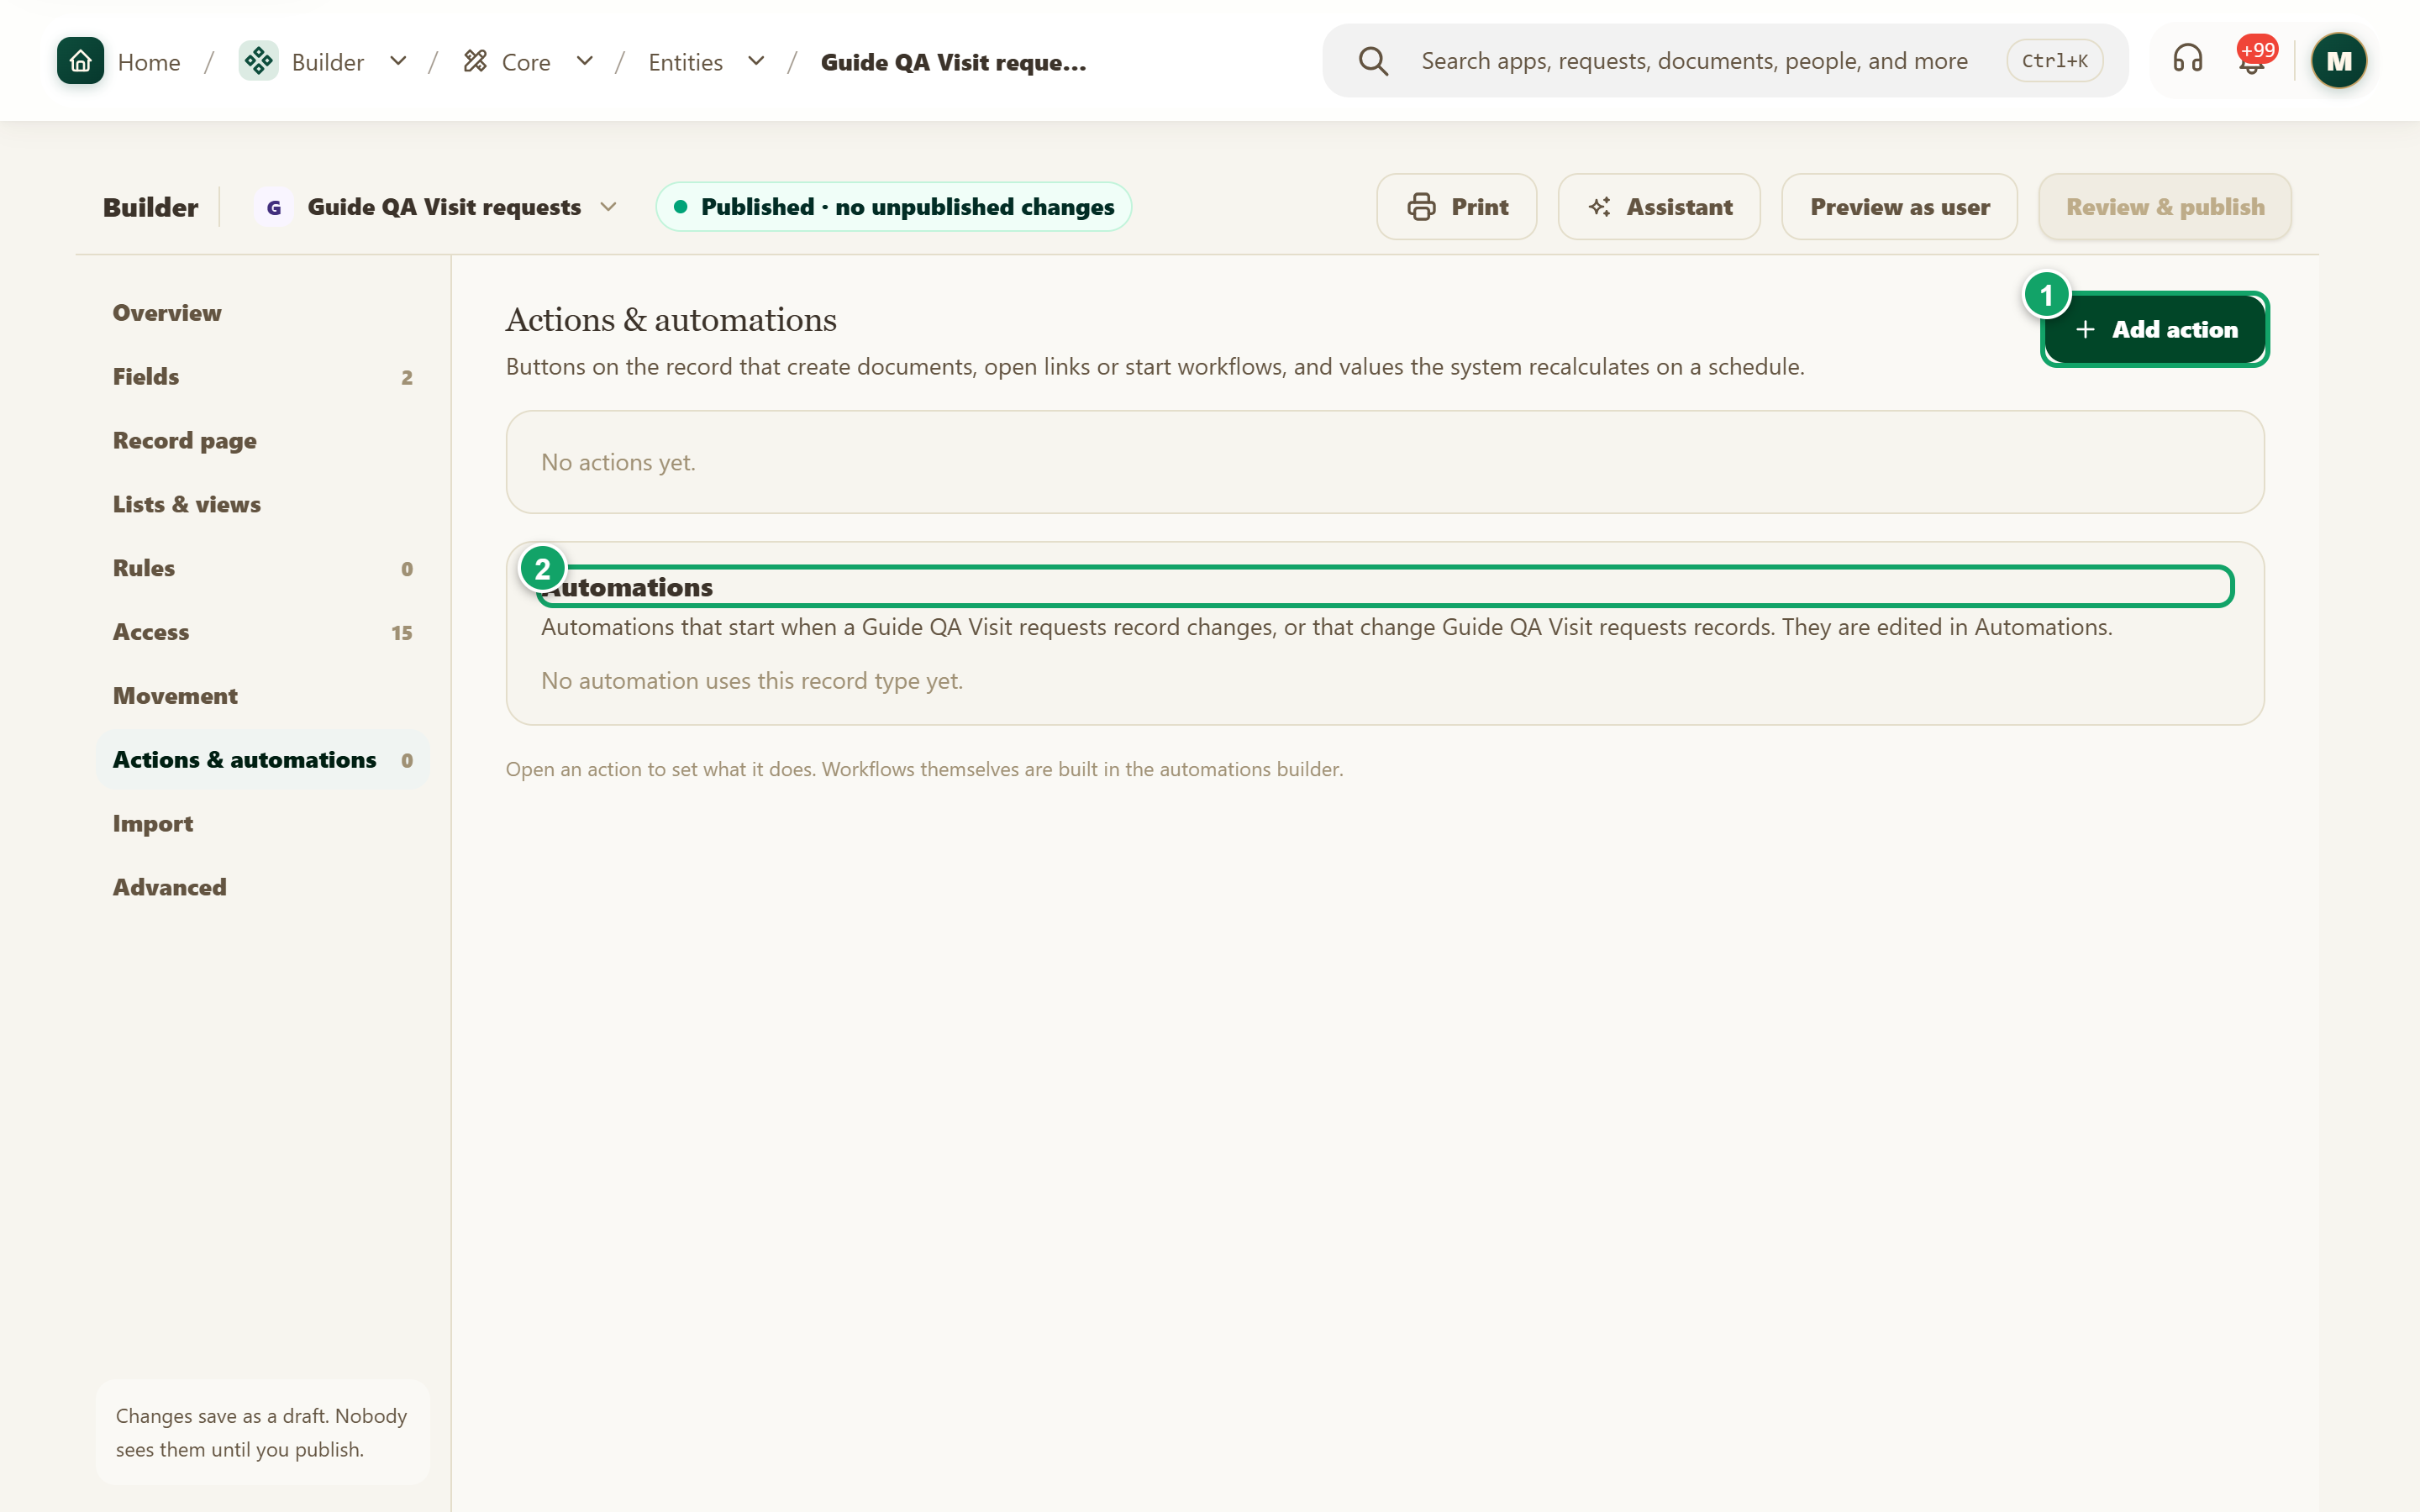
\includegraphics[width=0.95\linewidth,height=0.72\textheight,keepaspectratio]{figures/screens/ch06-ws-actions-en.png}
\caption{The “Actions \& automations” section}
\label{fig:builder-actions-screen}
\shotnote{The section shows the type’s buttons and its linked automations, both empty on the test type. ① “Add action”: creates a new button and opens it so you set what it does. ② “Automations”: a view-only list of automations started by, or changing, this type’s records.}
\end{figure}


\begin{table}[H]
\centering
\caption{What do you find here?}
\label{tab:builder-actions-data}
\begin{tabularx}{\linewidth}{R{3.6cm} Y}
\rcHeaderRow
\thh{Part} & \thh{Content and action}\\
Actions & Each action shows its kind, “Word document”, “Spreadsheet”, “Link” or “Workflow”, and who can run it: it “Needs” a given verb, or “Anyone who can change the record”.\\
Add action & Creates a “New action” in the draft and opens it in “Fields”, where you choose what it does and the template or workflow it uses.\\
Automations & A view-only list of automations that “Starts on a change” of a record of this type or that “Changes records”, with their state: “Live”, “Not published” or “Paused”. They are edited on the automations page.\\
Recalculated on a schedule & Calculated fields the system recalculates “Daily”, “Weekly” or “Monthly”; shown only when they exist.\\
\end{tabularx}
\end{table}

\begin{figure}[H]
\centering
\begin{tikzpicture}[node distance=0.5cm]
\node[entity] (action) {Action button on the record};
\node[entityOpt,below right=0.7cm and 0.3cm of action] (tpl) {Document template};
\node[entityOpt,below left=0.7cm and 0.3cm of action] (sop) {Workflow};
\draw[dependsOnOpt] (action.south) -- ++(0,-0.3) -| (tpl.north);
\draw[dependsOnOpt] (action.south) -- ++(0,-0.3) -| (sop.north);
\end{tikzpicture}
\rclegend
\caption{What an action calls}
\label{fig:builder-actions-model}
\shotnote{The figure shows that the button does not work on its own but calls something ready: a document template you prepare on the template pages, or a workflow you build in automations. So prepare the template or workflow first, then create the action and link it.}
\end{figure}

\subsection{Steps and check}
\begin{enumerate}
\item Prepare the template or workflow the button will call.
\item Open the record type, choose “Actions \& automations”, then press “Add action”.
\item In the field that opens, name the action, choose its kind and the template or workflow, then set the verb needed to run it.
\item Publish the changes, then open a test record and press the button.
\end{enumerate}

\textbf{Check and recovery:} the button should appear on the record for those holding the required verb, and it should produce the document or start the workflow. If the action shows the kind “Not set up”, open it and finish choosing what it does; if the button does not appear for a user, review the verb it needs.

\clearpage
\section{Movement}
\label{sec:builder-feature-movement}

Movement is a specialist setting for records that move an amount or quantity from one record to another, such as transfers between budget lines or between stores. Each record names where the amount comes from and where it goes; KayanOS keeps both sides equal and posts them together when the record reaches a status you choose. Most record types do not need this section. If you turn on “Evidence” on the same type, movement must post at the verify status, as page \ref{sec:builder-feature-evidence} explains.

\textbf{Path and who uses it:} record type → “Movement”. Used by whoever builds financial or stock record types.

\begin{rcnote}[Example: Horizon]
“Visit requests” does not need movement. But if Horizon created a type for transfers between branch budget lines, each approved transfer would post the amount from the Aleppo line to the Damascus line in one step. The system administrator does not go past the conditions in ②, because the requests type does not need them.
\end{rcnote}

\begin{figure}[H]
\centering
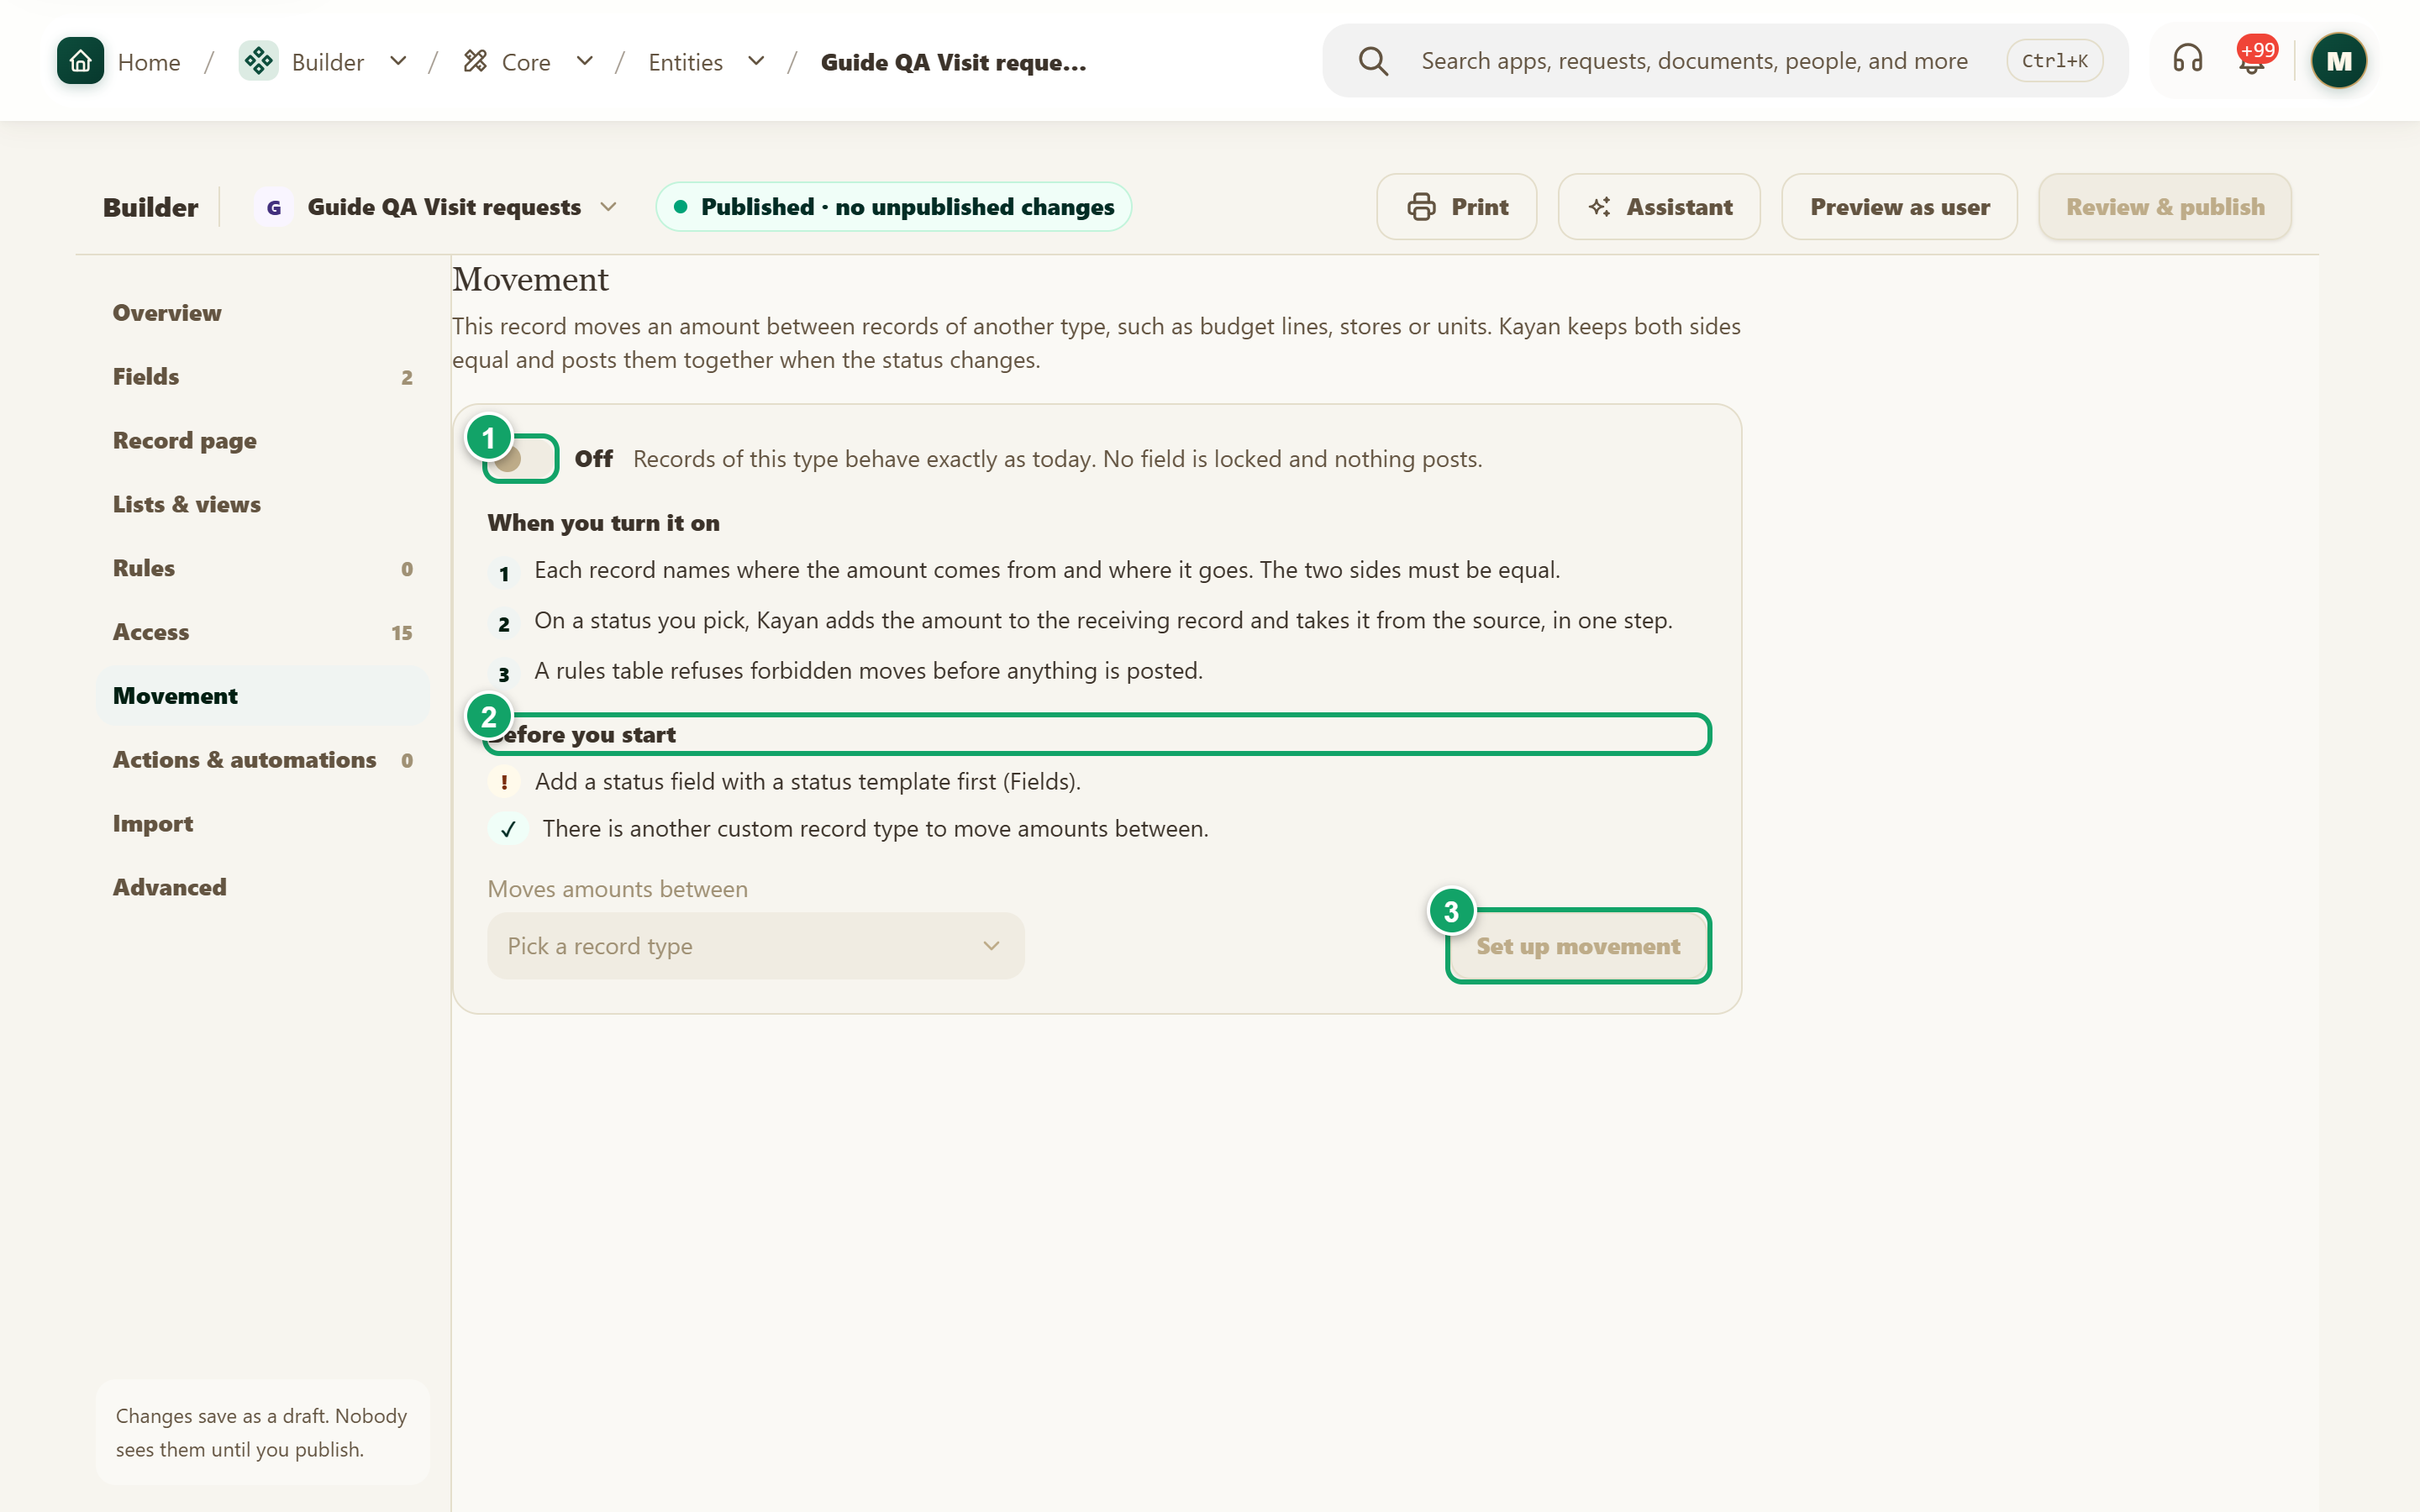
\includegraphics[width=0.95\linewidth,height=0.72\textheight,keepaspectratio]{figures/screens/ch06-ws-movement-en.png}
\caption{The “Movement” section while off}
\label{fig:builder-movement-screen}
\shotnote{The section explains what movement does once on and checks its conditions before you start. The warning mark shows because the test type has no status field. ① The switch: off, so nothing posts. ② “Before you start”: the conditions to meet, with a mark for each. ③ “Set up movement”: starts the setup after you choose the type amounts move between.}
\end{figure}


\begin{table}[H]
\centering
\caption{What do you need and set?}
\label{tab:builder-movement-data}
\begin{tabularx}{\linewidth}{R{3.6cm} Y}
\rcHeaderRow
\thh{Part} & \thh{Meaning}\\
Before you start & A “Status” field with a status template on this type, and another custom record type amounts move between, with number fields for “in” and “out”. Movement does not work on built-in types.\\
Sides & Where the amount comes from and where it goes; the two must be equal.\\
Posting & The status at which the amount posts, and its effect: hold, post, release or reverse.\\
Rules & Refuses forbidden moves before anything is posted.\\
Period totals and Try it & Show totals for each period and test the setup before publishing.\\
\end{tabularx}
\end{table}

\begin{figure}[H]
\centering
\begin{tikzpicture}[node distance=0.5cm]
\node[stepBox] (a) {Movement record: draft};
\node[stepBox,below=of a] (b) {Reaches the posting status};
\node[stepBox,below=of b] (c) {Taken from source, added to receiver};
\draw[flowsTo] (a) -- (b);
\draw[flowsTo] (b) -- (c);
\end{tikzpicture}
\rclegend
\caption{When does the amount move?}
\label{fig:builder-movement-flow}
\shotnote{The diagram shows that the amount does not move when the record is created but when it reaches the status you chose for posting. At that point it is taken from the source and added to the receiver together, so one side never moves without the other.}
\end{figure}

\subsection{Steps and check}
\begin{enumerate}
\item Make sure the “Status” field and the receiving record type with in and out fields exist.
\item Open “Movement”, choose the type in “Moves amounts between”, then press “Set up movement”.
\item Set the “Sides”, “Posting” and “Rules” tabs, then use “Try it” before publishing.
\end{enumerate}

\textbf{Check and recovery:} after publishing, move a test record to the posting status and confirm both balances changed by the same amount. If you turn movement off later, amounts already posted stay as they are and only new records stop posting.

\clearpage
\section{Evidence}
\label{sec:builder-feature-evidence}

“Evidence” is a specialist section for record types that record an amount paid or received, such as expense claims, which documents must prove. The section calls each record of such a type an “entry”: the submitter attaches the required documents and submits it, and KayanOS checks the documents and duplicates, numbers the entry and freezes its files. A verifier then answers a checklist for each document, and the verifier is never the entry's creator or submitter. After verification the entry locks for everyone, and corrections are reversal entries, never edits.

The section starts “Off”, so records work as before and no file is checked. The “Turn on” button works only with two conditions that the section lists under “Before you start”: a status field with a status template, and a number field for the amount. Evidence is not available on the system's built-in record types.

\textbf{Path and who uses it:} Builder workspace → “Evidence”. Whoever builds financial record types sets it up with the finance owner. After publishing, the record page shows an “Evidence” tab, where the submitter uploads the documents and presses “Submit for verification”, and the verifier verifies the entry or returns it for correction.

\begin{rcnote}[Example: Horizon]
“Visit requests” does not need evidence because it records no amount. But if Horizon created a type for visit expenses, the system administrator would make a “Hotel invoice” document always required, with the checklist item “Invoice is in the company's name”. Omar Haddad uploads the invoice for his Aleppo Branch visit and submits the entry, then Sarah Al-Khatib verifies it.
\end{rcnote}

\begin{figure}[H]
\centering
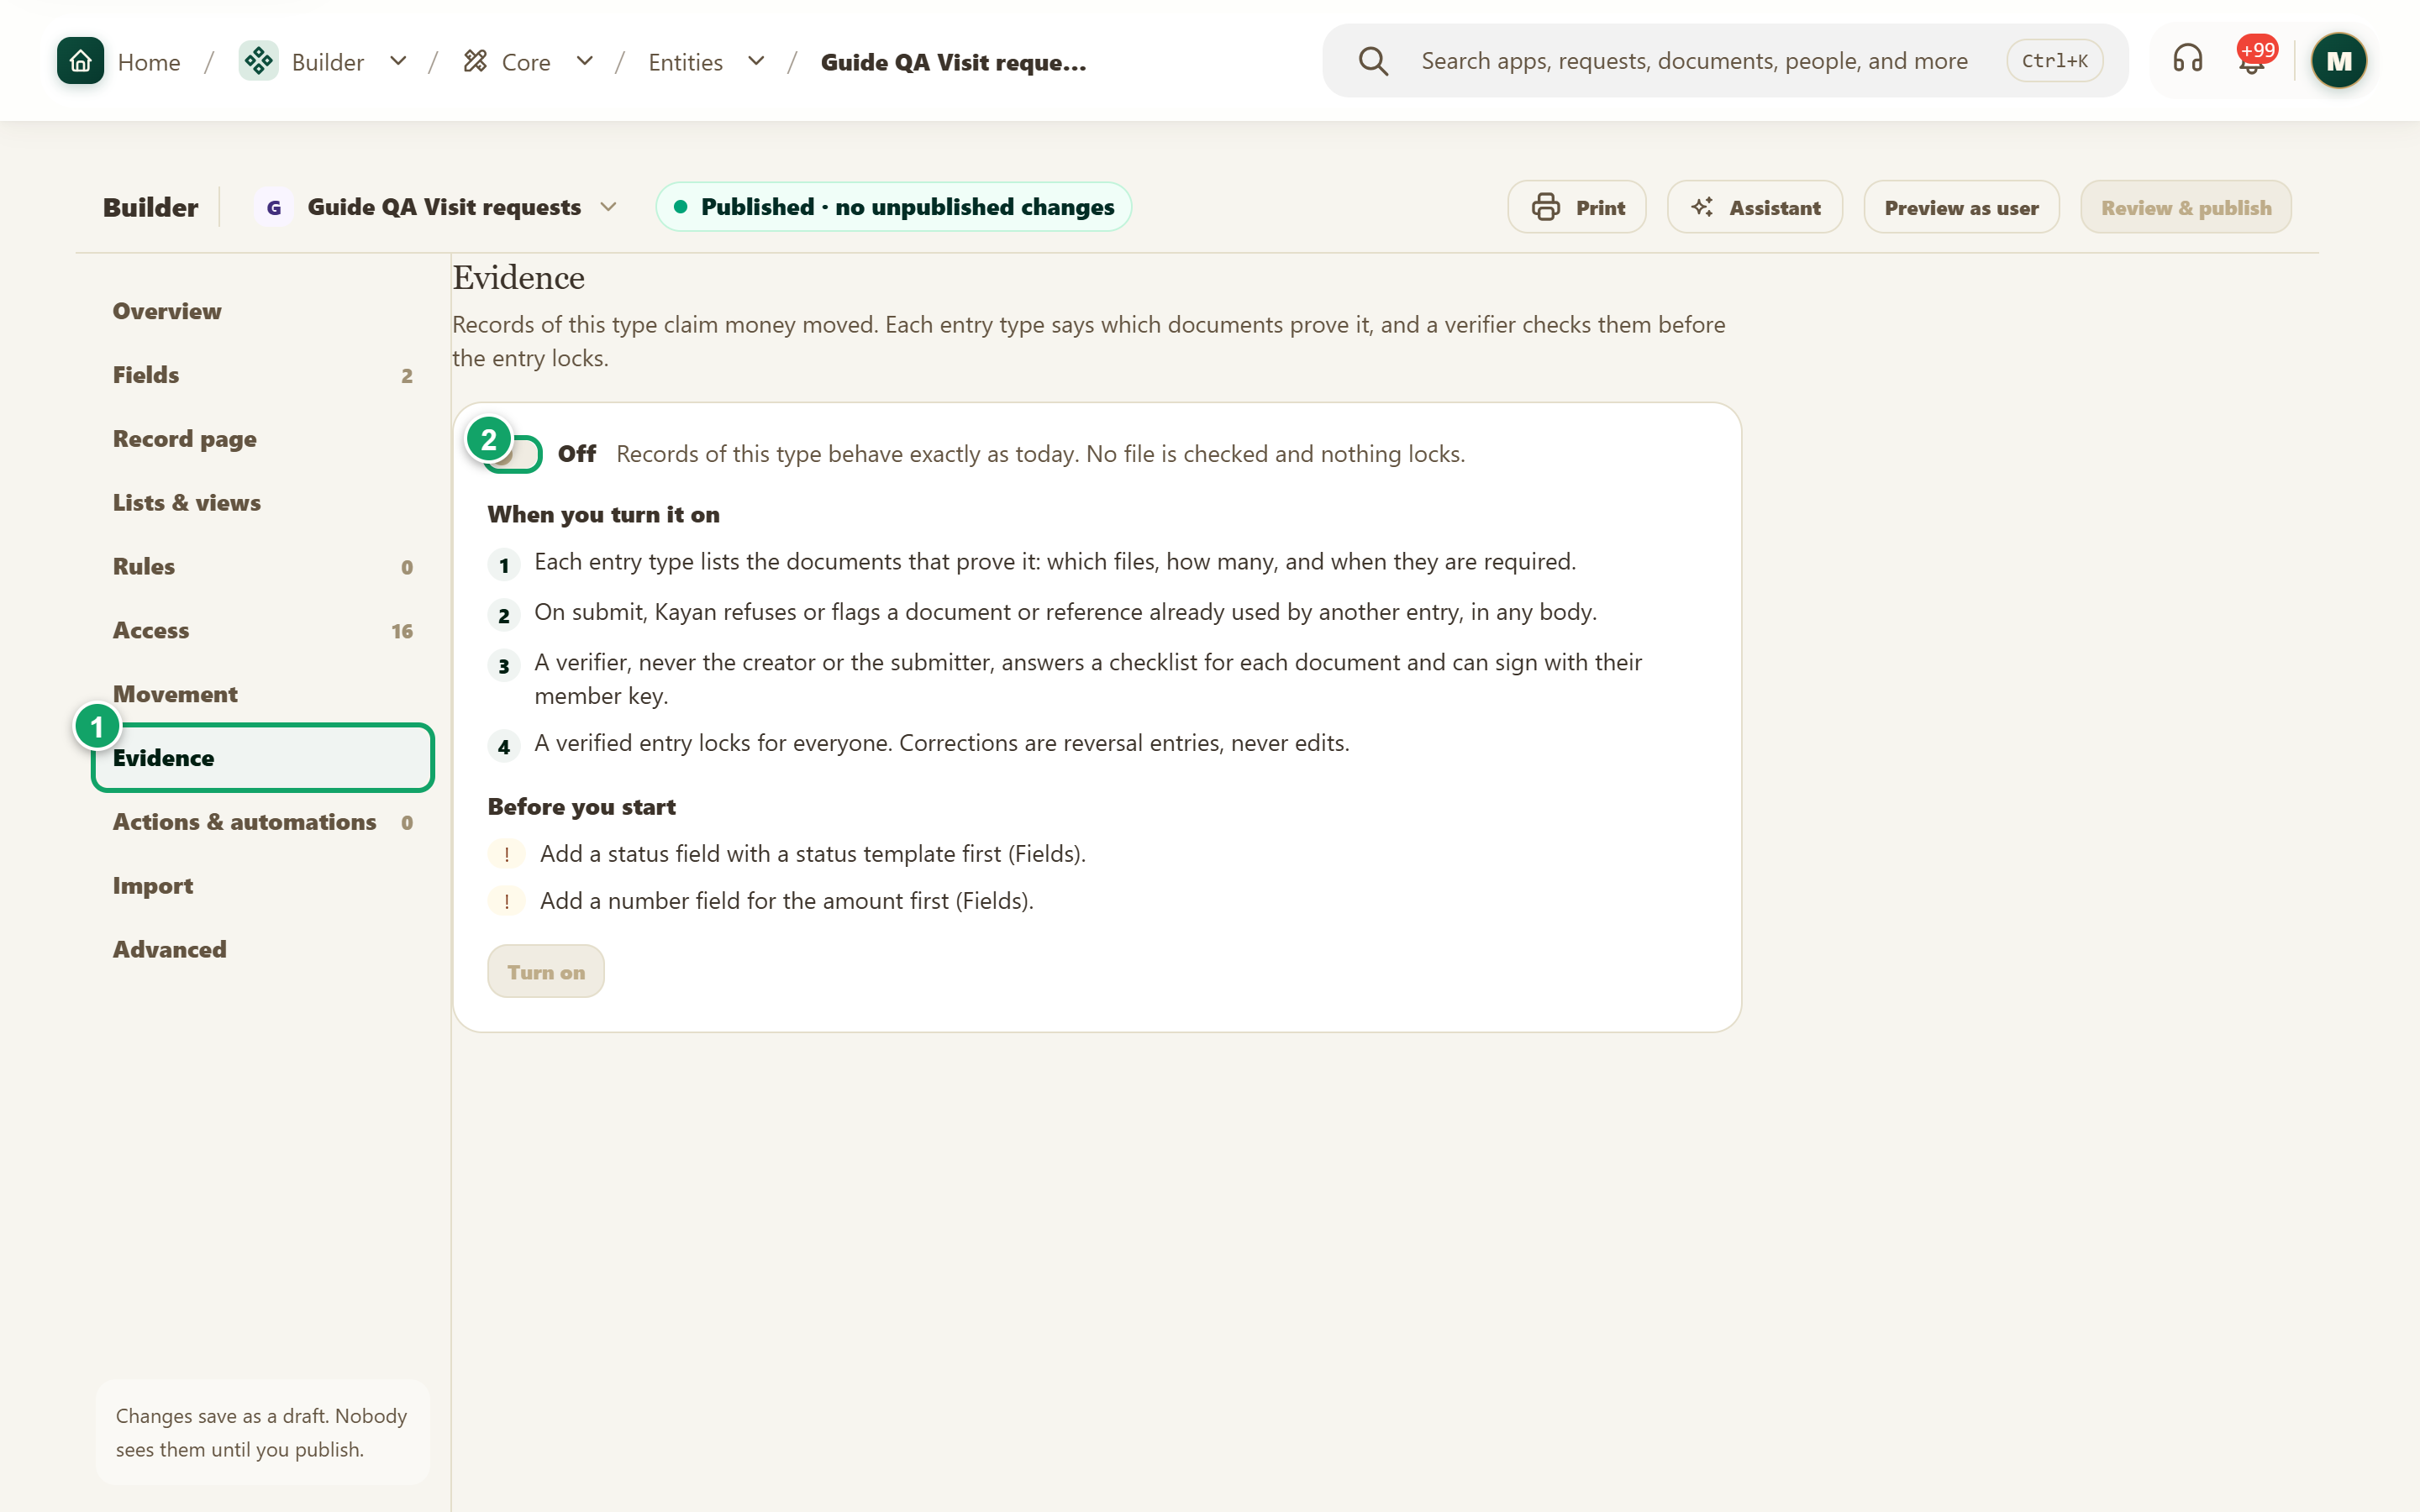
\includegraphics[width=0.95\linewidth,height=0.72\textheight,keepaspectratio]{figures/screens/ch06-ws-evidence-en.png}
\caption{The “Evidence” section before it is turned on, in a test record type}
\label{fig:builder-evidence-screen}
\shotnote{The image shows the section in the test type on test2 while it is off, with what happens once it is turned on and the “Before you start” list. It shows that the button stays disabled until both conditions are met, because this type has no status field and no number field for an amount. ① “Evidence” in the side menu. ② “Turn on”: switches evidence on once the conditions are met.}
\end{figure}

\begin{table}[H]
\centering
\caption{The “Evidence” tabs once it is on}
\label{tab:builder-evidence-tabs}
\begin{tabularx}{\linewidth}{R{3.6cm} Y}
\rcHeaderRow
\thh{Tab} & \thh{What you set there}\\
Entry types \& slots & Under “General”: “Status field”, “Submit status”, “Verify status” and “Return statuses”, an “Entry type field” when documents differ by entry type, “Entry fields” (the amount is required; currency, value date, body and counterparty are optional) and “Numbering” with a prefix. Then the entry types, each with its “Cross-checks” and “Evidence slots”.\\
Duplicates & Rules that compare each submitted entry with the type's entries by “File content”, “Fields” or “AI reading”, within the “Same body” or the “Whole organization”, then “Refuse”, “Warn, reason” or “Flag for verifier”. When several rules match, the strictest outcome wins.\\
AI reading & AI reads values such as the “Total amount” and “Document number” from the documents, then suggests them or compares them with what the submitter typed, within a “Monthly cap” and “Pages per file”.\\
Posting & Shows the “Lifecycle” from submit to return or verify, and checks the status template and its agreement with the “Movement” section. Without a movement setup, entries are proved, verified and locked, and no amount moves.\\
Confidentiality & The “Default level” for documents, the “Verifier signature” with the member key, and “Editable after verification” for fields that stay open after the lock, such as notes. Documents at level “Secret (3)” and above can only be viewed: never downloaded and never sent to AI reading.\\
\end{tabularx}
\end{table}

\begin{table}[H]
\centering
\caption{The settings of each slot}
\label{tab:builder-evidence-slot}
\begin{tabularx}{\linewidth}{R{3.6cm} Y}
\rcHeaderRow
\thh{Setting} & \thh{Meaning}\\
Required & “Always”, “Optional”, or “When…” a condition holds, checked on submit and again on verify.\\
Files & The accepted formats: PDF, images, Word and Excel; the number of files “At least” and “At most”; the “Max size (MB)”; and a minimum photo resolution. With no format picked, PDF and images are accepted.\\
Shared document & “May back other entries” when one document covers more than one entry, such as instalments.\\
Confidentiality and reading & A confidentiality level for the slot, and “AI reads this slot”.\\
Verifier checklist & Items the verifier answers with yes, no or not applicable plus a note; verification completes only when every answer is yes or not applicable.\\
\end{tabularx}
\end{table}

\begin{rcwarn}[Turning it off keeps what was submitted]
If you turn evidence off after entries were submitted, KayanOS keeps the setup and the section shows “Turned off” with a “Turn on again” button; the entries' history and locks stay as they are. Evidence files are never deleted: even a returned entry keeps its old files beside the new ones.
\end{rcwarn}

\subsection{Checklists with evidence}

“Evidence” fits financial entries only. If you want a list of items answered inside a record, some of which need a photo or file as proof, such as a visit checklist, make the items related records and set them up from the “Relation” field on the item type: choose “Show relation in tab”, then “Checklist” under “Relations display”. You then set the “Answer field”, pick under “Evidence files” the “File collection” the proof is uploaded to, and add a condition under “Evidence is required only when…” if needed.

\begin{figure}[H]
\centering
\begin{tikzpicture}[node distance=0.5cm]
\node[stepBox] (a) {Status and amount fields};
\node[stepBox,below=of a] (b) {Turn evidence on};
\node[stepBox,below=of b] (c) {Entry types and slots};
\node[stepBox,below=of c] (d) {Duplicates and confidentiality};
\node[stepBox,below=of d] (e) {Posting with Movement};
\node[stepBox,below=of e] (f) {Review and publish};
\draw[flowsTo] (a) -- (b);
\draw[flowsTo] (b) -- (c);
\draw[flowsTo] (c) -- (d);
\draw[flowsTo] (d) -- (e);
\draw[flowsTo] (e) -- (f);
\end{tikzpicture}
\rclegend
\caption{Turning evidence on and setting it up}
\label{fig:builder-evidence-flow}
\shotnote{The diagram starts with the two fields because the turn-on button stays disabled without them, and because KayanOS infers the submit and verify statuses and the amount field from them. Posting comes before publishing because KayanOS refuses to publish when evidence disagrees with the “Movement” setup, so money moves only after verification.}
\end{figure}

\subsection{Steps and check}
\begin{enumerate}
\item In “Fields”, make sure there is a “Status” field with a fixed, published template that has a status for submitting and another for verifying, and a “Number” field for the amount.
\item Open “Evidence” and press “Turn on”, then review under “General” the statuses KayanOS suggested, and pick the “Entry fields” and the “Prefix”.
\item Under “Evidence slots”, press “Add slot” for each document, set “Required” and the files, then add “Verifier checklist” items with “Add item”.
\item Review “Duplicates” and “Confidentiality”, then open “Posting” and resolve every check that is not met, especially if the type has a “Movement” setup.
\item Publish, then create a test record, upload its documents in the “Evidence” tab, press “Submit for verification”, and ask another user to verify it.
\end{enumerate}

\textbf{Check and recovery:} a “Ready” badge should appear next to the section title, and the submitted entry should carry a number that starts with your prefix. If “Turn on” stays disabled, add the field that “Before you start” points to. If a badge shows the number of problems “to fix”, or “Evidence setup” appears in “Before you publish”, open the tab marked with an error and complete what is missing.

\clearpage
\section{Import}
\label{sec:builder-feature-import}

The “Import” section decides how people load and update this type's records from Excel and CSV files. Its core is “Import keys”: a field or set of fields, such as a code or number, that KayanOS uses to match each row in the file to an existing record, so it updates that record instead of creating a duplicate. When the option is off, import works as before and guesses matches by ID, code or name.

\textbf{Path and who uses it:} record type → “Import”. Used by whoever builds the record type, before the team starts updating records from files.

\begin{rcnote}[Example: Horizon]
The system administrator adds an import key based on the request number \en{HZN-VR-0001}, so Omar Haddad uploads an Excel file with updated visit dates and KayanOS updates the same requests without creating new ones. They add the key from ② and check it with ③.
\end{rcnote}

\begin{figure}[H]
\centering
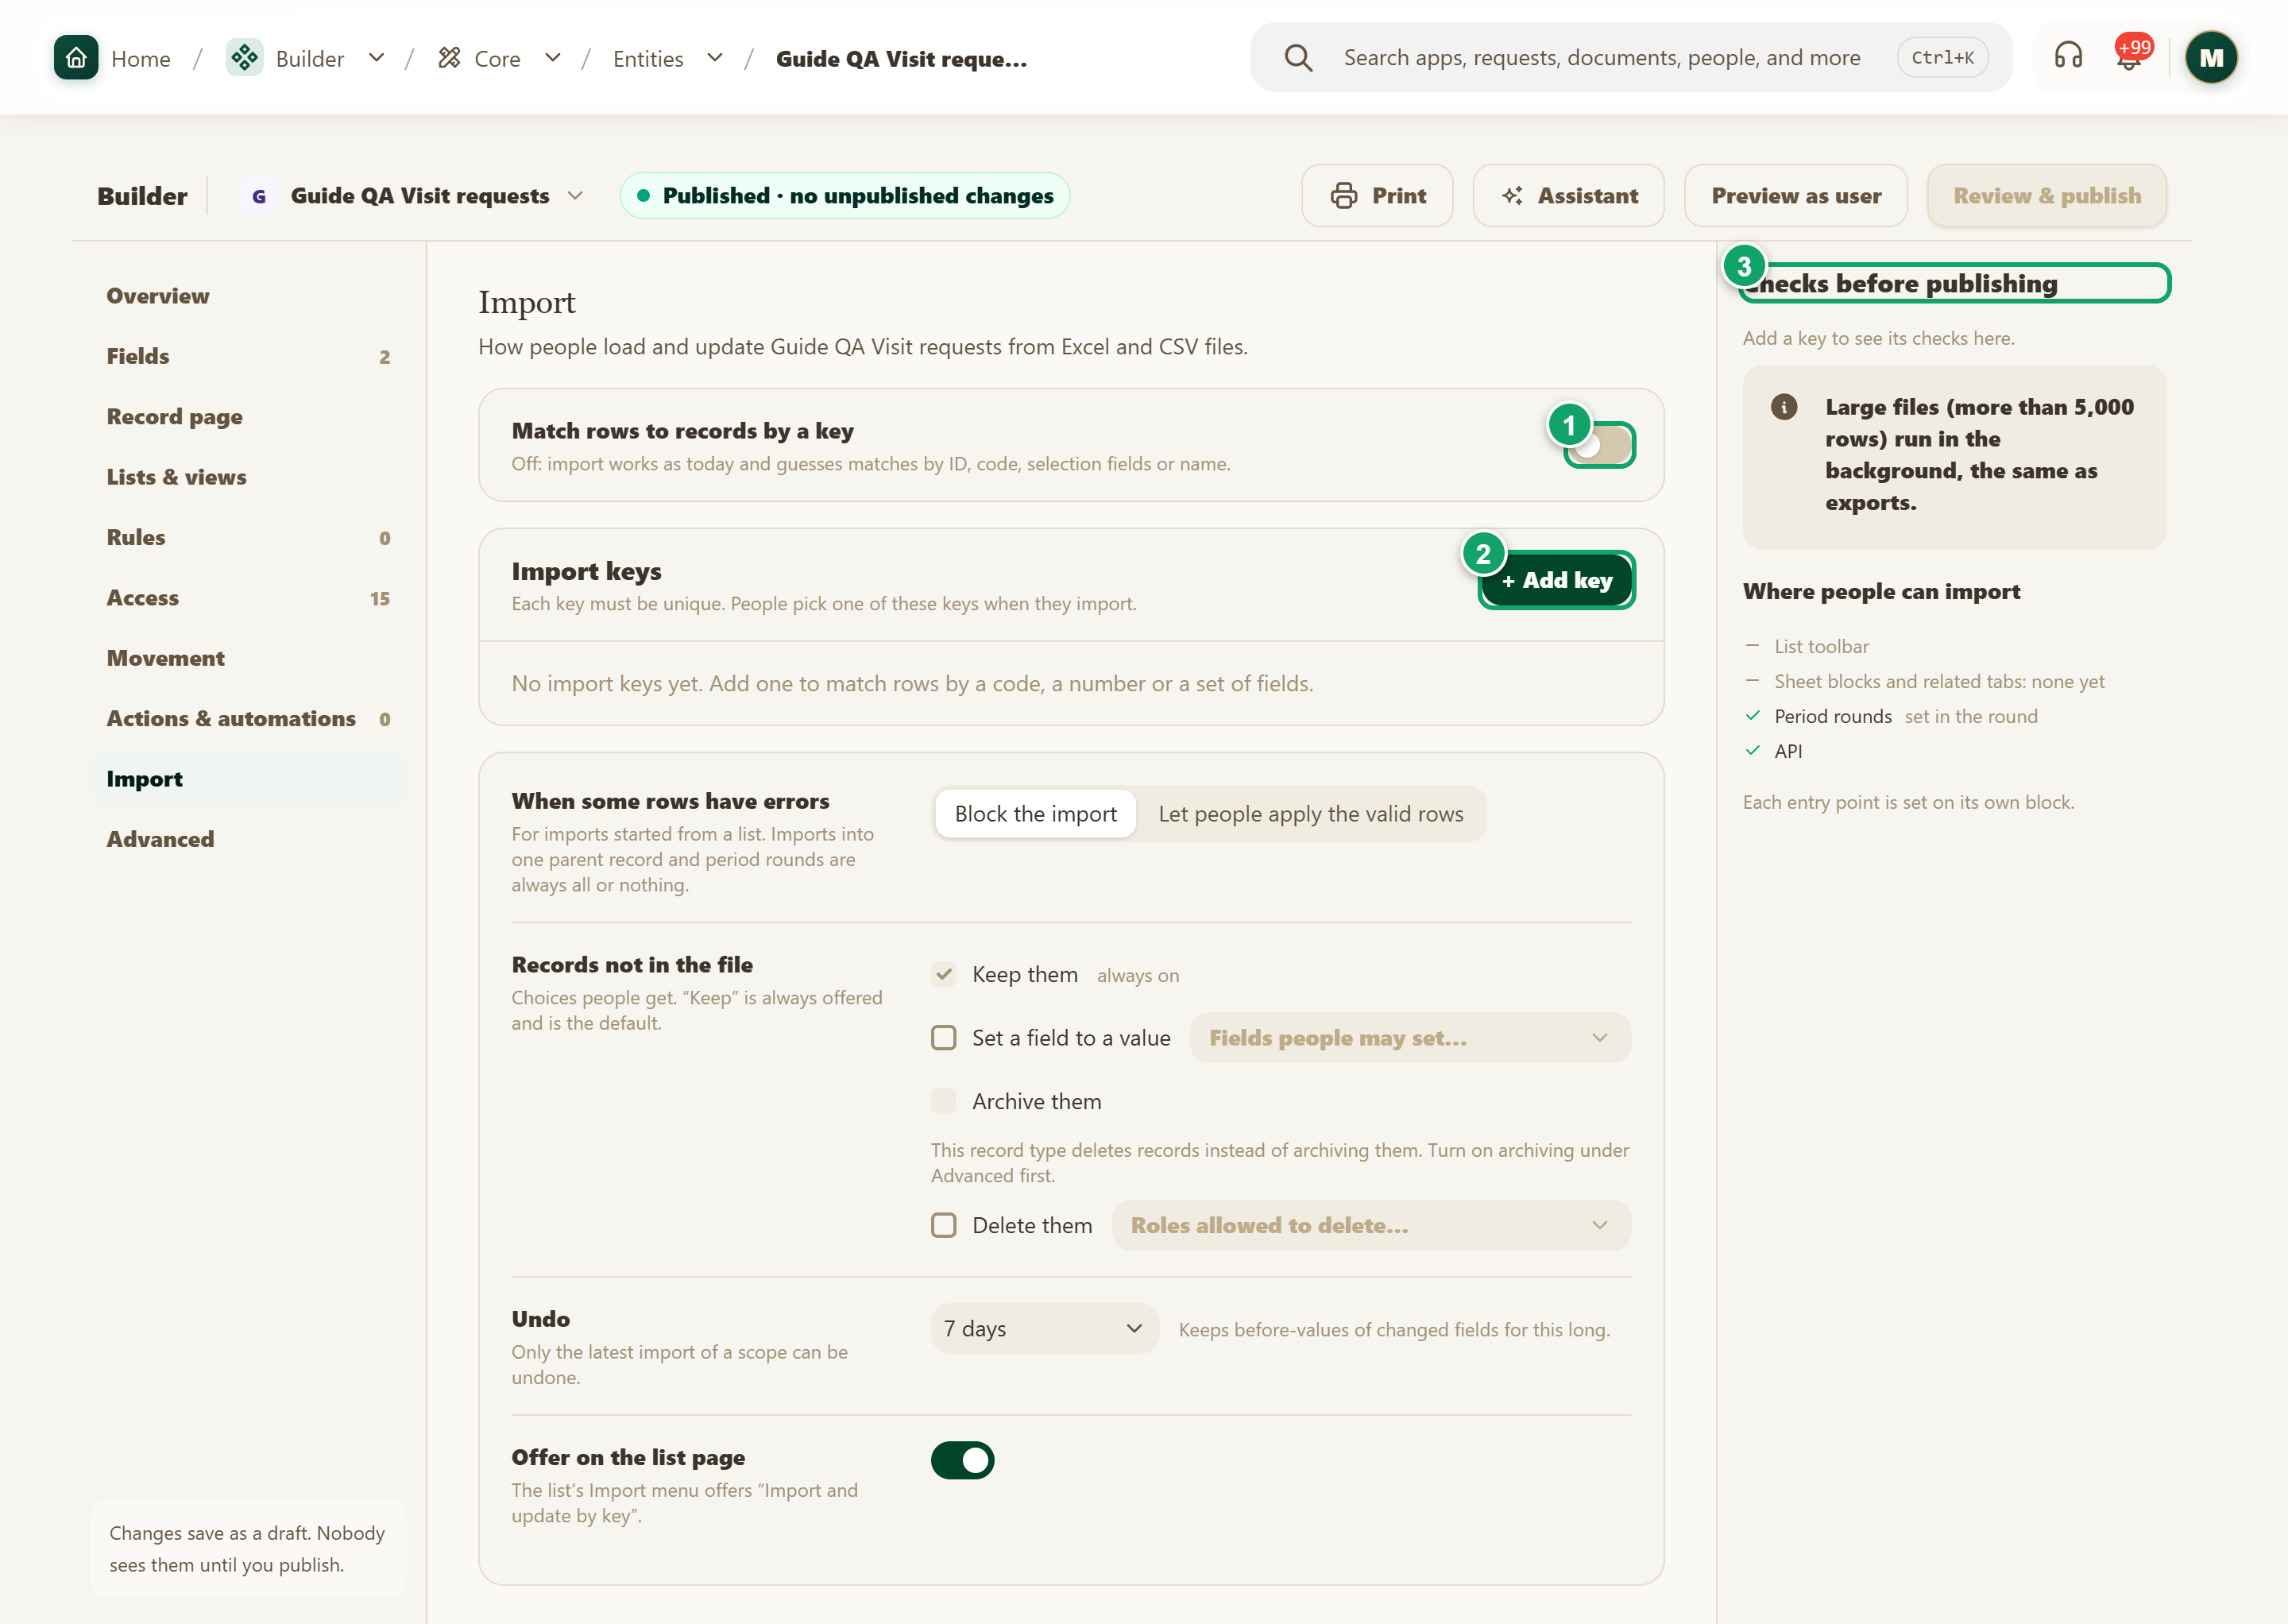
\includegraphics[width=0.95\linewidth,height=0.72\textheight,keepaspectratio]{figures/screens/ch06-ws-import-en.png}
\caption{The “Import” section}
\label{fig:builder-import-screen}
\shotnote{The section decides how records are updated from Excel and CSV files; matching by key is off here. ① The “Match rows to records by a key” switch. ② “+ Add key”: adds the field rows are matched by. ③ “Checks before publishing”: after you add a key, “Run the check” shows here whether it is unique among saved records.}
\end{figure}


\begin{table}[H]
\centering
\caption{What do you find here?}
\label{tab:builder-import-data}
\begin{tabularx}{\linewidth}{R{3.6cm} Y}
\rcHeaderRow
\thh{Part} & \thh{Content and action}\\
Match rows to records by a key & Turns on import by key. When off, import guesses matches as before.\\
Import keys & Each key shows the fields it is “Made of”, where it is “Unique within”, its “Normalising”, such as ignoring spaces or leading zeros, whether it is “Backed by” a unique value, and its status, “Ready” or “Problem”.\\
Behaviour & What happens “When some rows have errors”, block the import or allow the valid rows, what happens to records missing from the file, keep, archive or delete them, and how long the last import can be undone.\\
Checks before publishing & “Run the check” confirms the key is unique among saved records and shows duplicate or empty ones.\\
\end{tabularx}
\end{table}

\begin{figure}[H]
\centering
\begin{tikzpicture}[node distance=0.5cm]
\node[stepBox] (a) {Add an import key};
\node[stepBox,below=of a] (b) {Run the check};
\node[stepBox,below=of b] (c) {Set the behaviour};
\node[stepBox,below=of c] (d) {Publish, then import a file};
\draw[flowsTo] (a) -- (b);
\draw[flowsTo] (b) -- (c);
\draw[flowsTo] (c) -- (d);
\end{tikzpicture}
\rclegend
\caption{Preparing import by key}
\label{fig:builder-import-flow}
\shotnote{The diagram puts the check right after adding the key, because a key whose value repeats across two records cannot tell which one to update. Then you decide what happens to errors and to records missing from the file, because a wrong choice here can archive or delete records. None of it works before you publish.}
\end{figure}

\subsection{Steps and check}
\begin{enumerate}
\item Open the record type, choose “Import”, then turn on “Match rows to records by a key”.
\item Press “+ Add key” and choose the field that identifies each record, such as the code or serial number.
\item Press “Run the check” and fix any duplicate or empty records it shows.
\item Choose the right behaviour for errors and missing records, then publish the changes.
\end{enumerate}

\textbf{Check and recovery:} the key's status should be “Ready” and the check should show it is unique. If it shows that some records would share the same key, fix their values first. Only choose to delete records missing from the file on purpose, and use undo if an import goes wrong.

\clearpage
\section{Advanced}
\label{sec:builder-feature-advanced}

“Advanced” holds settings that rarely change after the start, such as the record's name in lists, preventing duplicates, parent–child records and the app where the type appears. They are part of the draft like the other sections, so they do not reach the team before publishing.

\textbf{Path and who uses it:} record type → “Advanced”. Used by whoever builds the type, usually at creation and then only when needed.

\begin{rcnote}[Example: Horizon]
The system administrator makes the visit request's “Record name” the serial number with the branch name, places the type in the “Branch services” app, and chooses “Archive records instead of deleting them” so no request is lost. Their choices match numbers ① and ④.
\end{rcnote}

\begin{figure}[H]
\centering
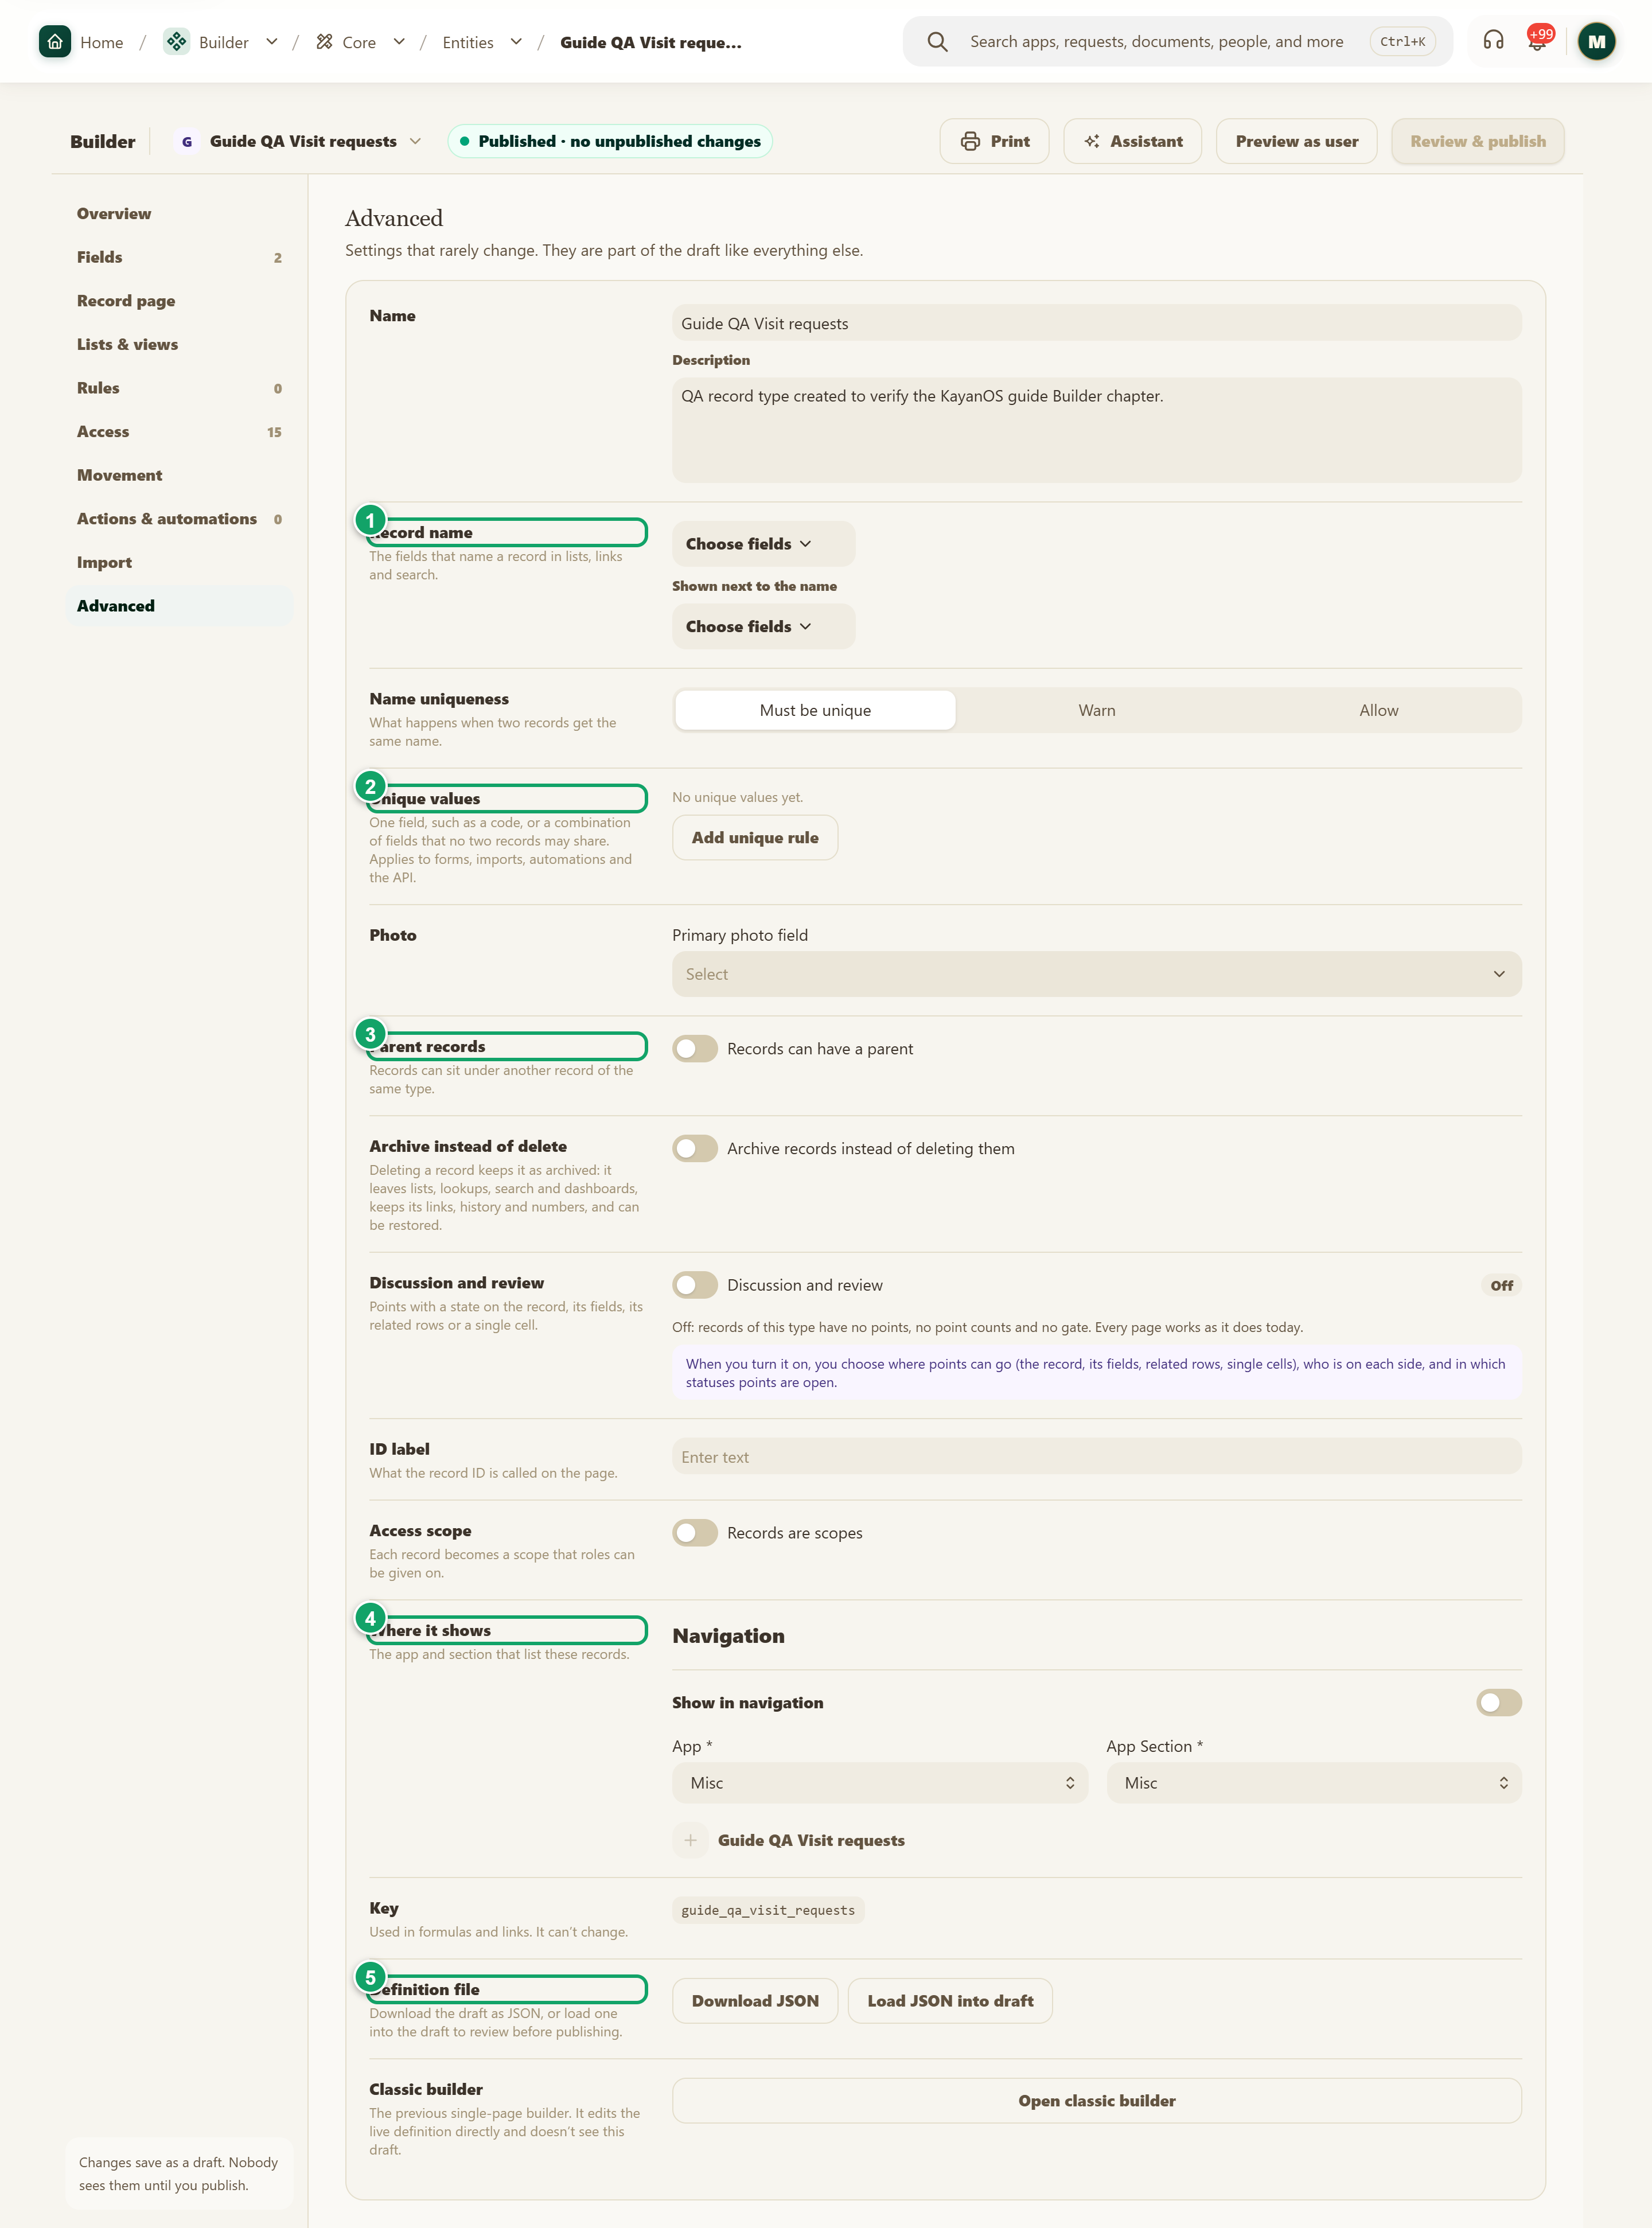
\includegraphics[width=0.95\linewidth,height=0.72\textheight,keepaspectratio]{figures/screens/ch06-ws-advanced-en.png}
\caption{The “Advanced” section}
\label{fig:builder-advanced-screen}
\shotnote{The section gathers rarely changed settings, shown here for the test record type. ① “Record name”: the fields that name a record. ② “Unique values”: prevents a repeated code or combination of values. ③ “Parent records”: allows parent–child records. ④ “Where it shows”: the app and section. ⑤ “Definition file”: download or load the setup as JSON.}
\end{figure}


\begin{table}[H]
\centering
\caption{What do you find here?}
\label{tab:builder-advanced-data}
\begin{tabularx}{\linewidth}{R{3.6cm} Y}
\rcHeaderRow
\thh{Setting} & \thh{Meaning}\\
Record name & The fields that name a record in lists, links and search, plus an optional field “Shown next to the name”.\\
Name uniqueness & What happens when two records get the same name: “Must be unique”, “Warn” or “Allow”.\\
Unique values & A field, such as a code, or a combination of fields that no two records may share, also in forms, imports and automations.\\
Photo & The field used as the record's main photo.\\
Parent records & Lets a record sit under another record of the same type, which makes the “Tree” view available.\\
Archive instead of delete & A deleted record stays archived: it leaves lists and search, keeps its links and numbers, and can be restored. You can also archive its child records and linked tasks with it.\\
Discussion and review & Lets people open points with a state on the record, its fields, its related rows or a single cell; they appear in a “Points” tab on the record page. It stays off until you turn it on.\\
ID label & What the record ID is called on the page.\\
Access scope & Makes each record a scope roles can be given on, such as giving a branch manager rights on their branch only.\\
Where it shows & The “App” and “App Section” that list the records, “Show in navigation”, and the icon.\\
Key & Used in formulas and links; it can't change.\\
Definition file & “Download JSON” for a copy of the draft, or “Load JSON into draft” to review it before publishing.\\
Classic builder & The previous single-page builder; it edits the live definition directly and doesn't see the draft, so use it with care.\\
\end{tabularx}
\end{table}

\begin{figure}[H]
\centering
\begin{tikzpicture}[node distance=0.5cm]
\node[entity] (adv) {Advanced};
\node[entityOpt,below right=0.7cm and 0.3cm of adv] (tree) {Parent records};
\node[entityOpt,below left=0.7cm and 0.3cm of adv] (scope) {Access scope};
\node[entityOpt,below=0.7cm of tree] (treeview) {Tree view};
\node[entityOpt,below=0.7cm of scope] (roles) {Roles on one record};
\draw[dependsOnOpt] (adv.south) -- ++(0,-0.3) -| (tree.north);
\draw[dependsOnOpt] (adv.south) -- ++(0,-0.3) -| (scope.north);
\draw[dependsOnOpt] (tree) -- (treeview);
\draw[dependsOnOpt] (scope) -- (roles);
\end{tikzpicture}
\rclegend
\caption{Two settings that unlock other features}
\label{fig:builder-advanced-effects}
\shotnote{The figure shows that some advanced settings are a condition for features in other sections: turning on “Parent records” makes the “Tree” view available in lists, and turning on “Access scope” allows roles on a single record. So if one of these features is missing, start by reviewing this section.}
\end{figure}

\subsection{Steps and check}
\begin{enumerate}
\item Open the record type and choose “Advanced”.
\item Choose a “Record name” from fields that really identify the record, such as the serial number.
\item Use “Add unique rule” for fields that must not repeat, and review the warning if duplicates already exist.
\item Review “Where it shows” to confirm the app and section, then publish the changes.
\end{enumerate}

\textbf{Check and recovery:} after publishing, records should appear in lists and search under the name you chose, and a duplicate unique value should be refused. Before any large change, use “Download JSON” to keep a copy of the setup.

\clearpage
\section{Review \& publish}
\label{sec:builder-feature-publish}

The “Builder” workspace saves every change as a draft, and nobody else sees those changes until you publish them. “Review \& publish” shows all the changes before publishing and blocks it while a problem remains to be fixed. Each publish creates a new version you can return to later.

\textbf{Path and who uses it:} record type → “Review \& publish”. Used by whoever builds the type after finishing a set of changes.

\begin{rcnote}[Example: Horizon]
Before launching “Visit requests”, the system administrator uses “Preview as user” to see the page as Omar Haddad sees it, publishes the first version and asks Omar to try a request for the Aleppo Branch visit. They use ③ before publishing from ④.
\end{rcnote}

\begin{figure}[H]
\centering
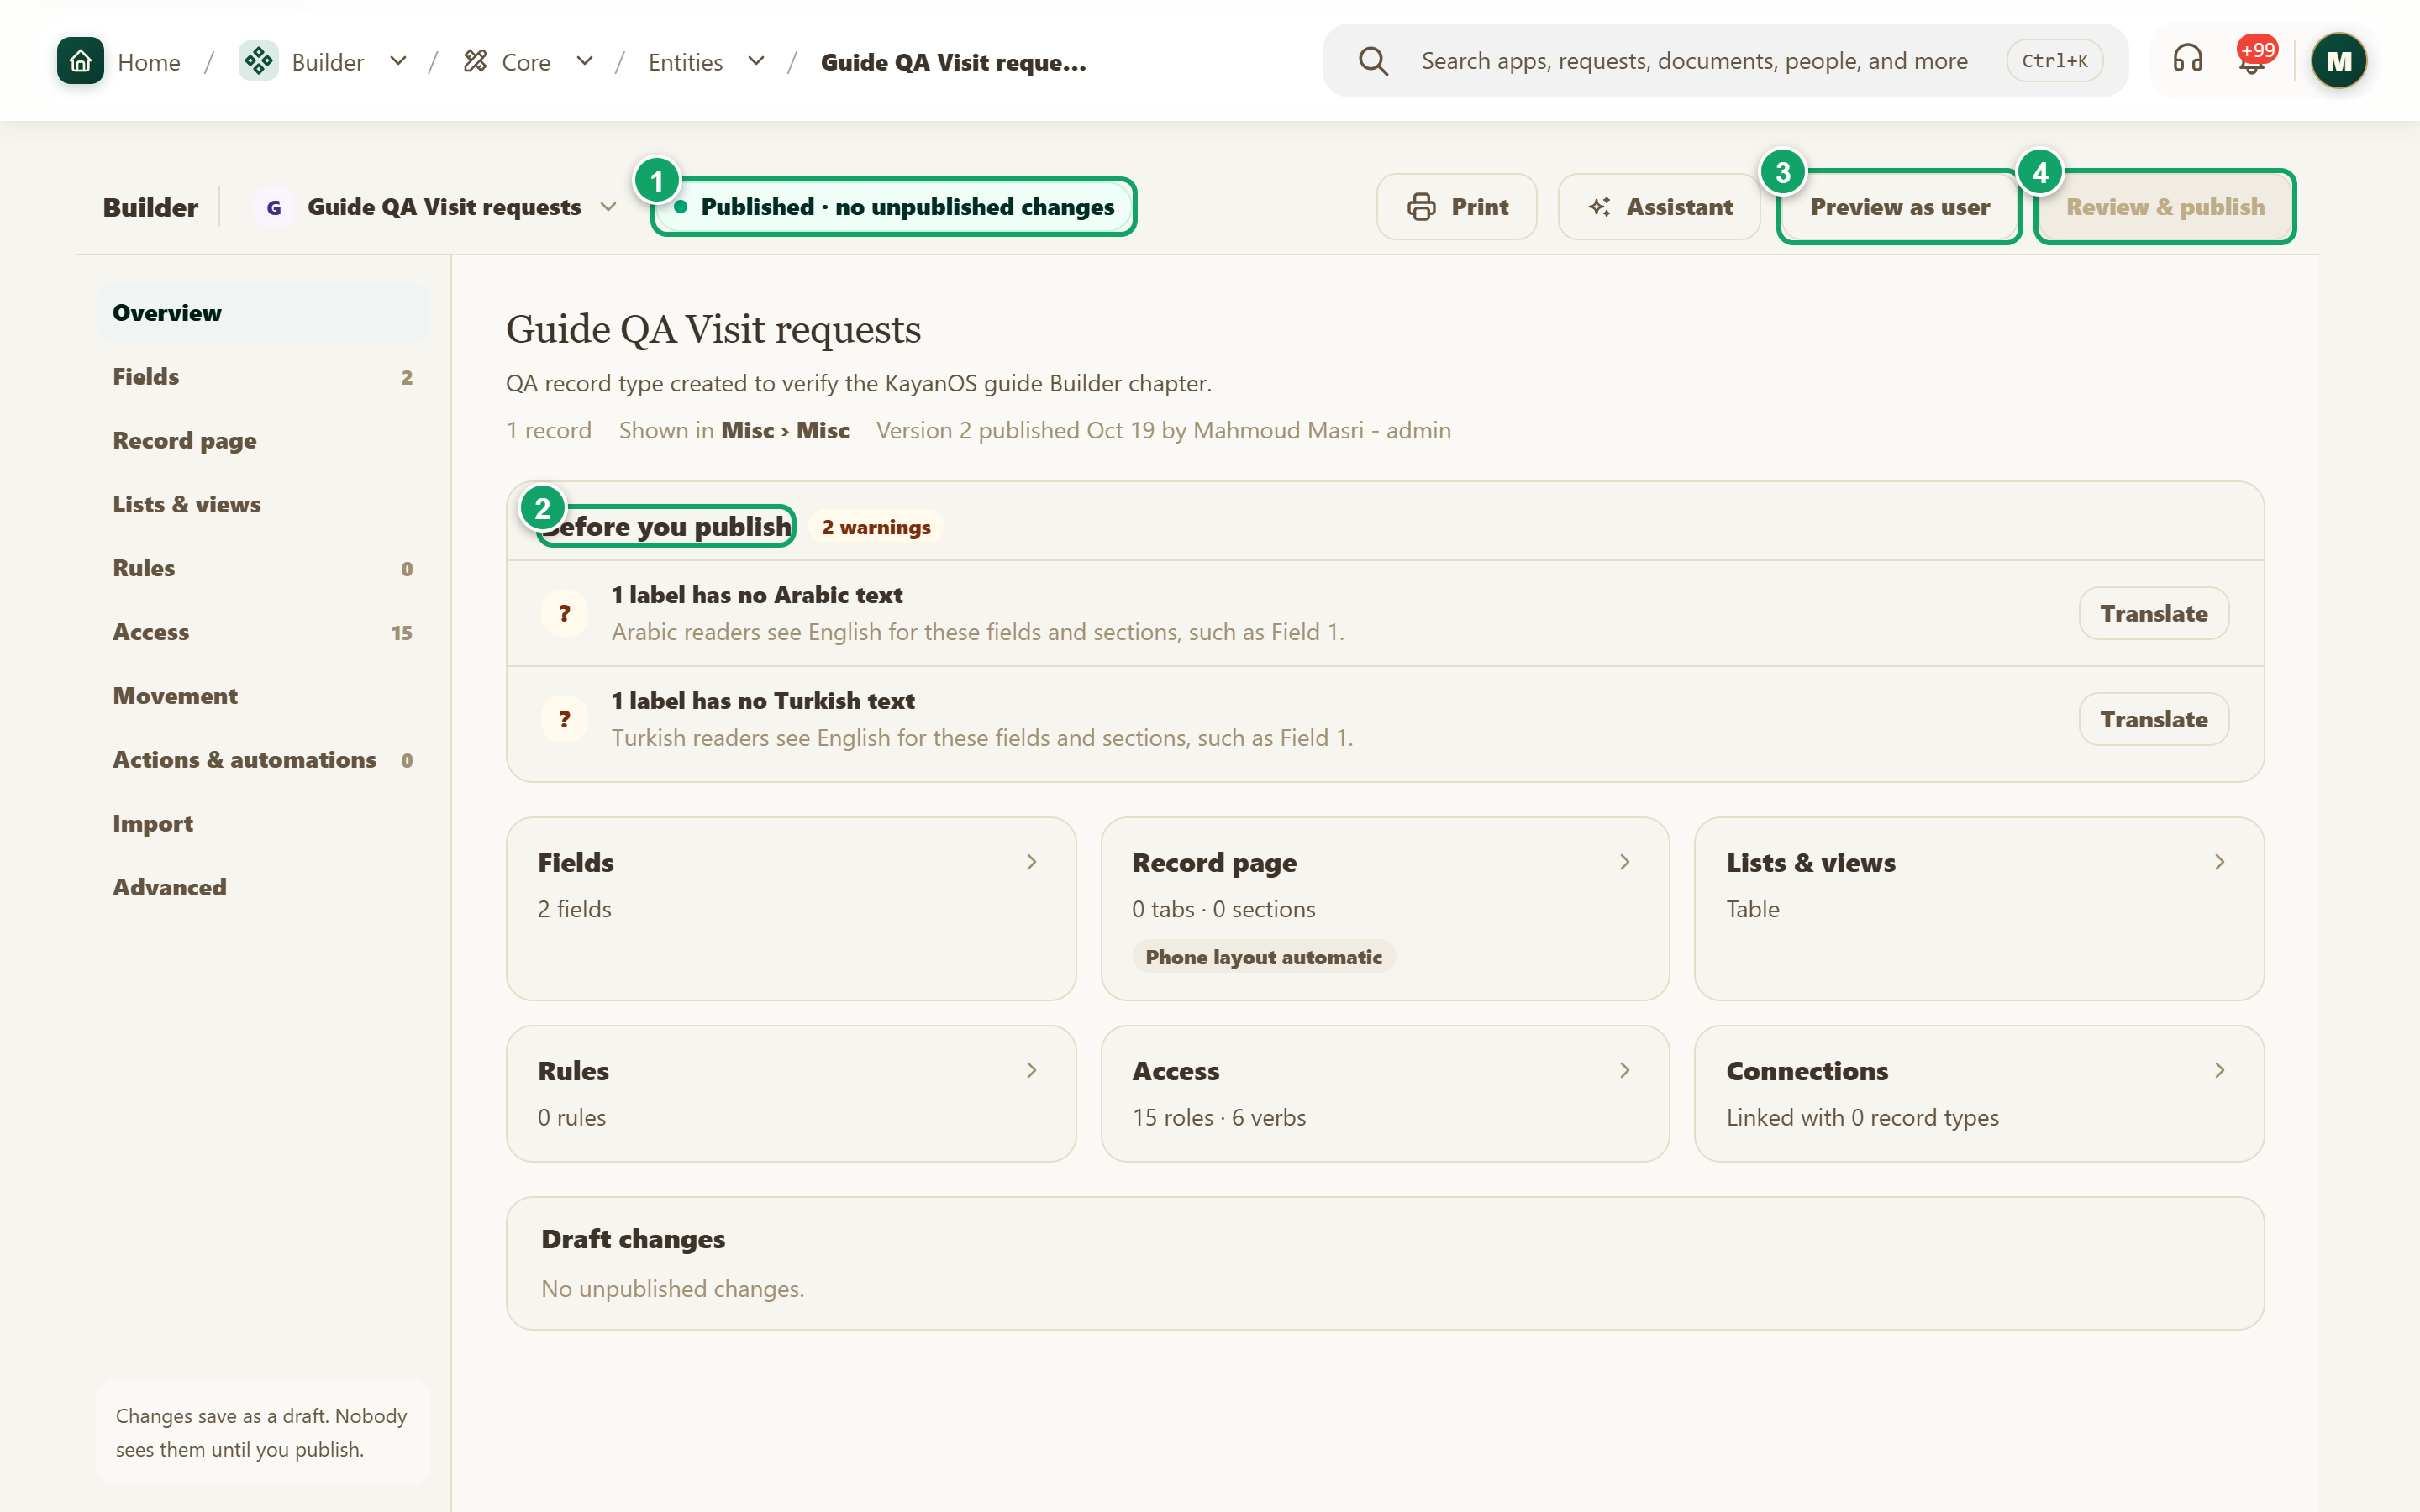
\includegraphics[width=0.95\linewidth,height=0.72\textheight,keepaspectratio]{figures/screens/ch06-ws-overview-en.png}
\caption{“Overview” after publishing}
\label{fig:builder-publish-screen}
\shotnote{“Overview” summarizes the type’s state and what to fix before publishing. The test type here is published as version 2 after testing this chapter, with translation warnings that do not block publishing. ① The state: “Published · no unpublished changes”. ② “Before you publish”: problems and warnings. ③ “Preview as user”. ④ “Review \& publish”: opens the change list and the publish button.}
\end{figure}


\begin{table}[H]
\centering
\caption{What do you find here?}
\label{tab:builder-publish-data}
\begin{tabularx}{\linewidth}{R{3.6cm} Y}
\rcHeaderRow
\thh{Item} & \thh{Meaning and action}\\
Draft & The type has unpublished changes. “Published · no unpublished changes” means the team sees the latest version you built.\\
Overview & A summary of fields, page, lists and rules; “Before you publish” lists the problems that block publishing and the warnings.\\
Preview as user & Shows the type as the user will see it, before publishing.\\
Review \& publish & Opens the review of changes grouped by section; each change has a checkbox you can clear to keep it in the draft. You add an optional description of the version, then press “Publish N changes”.\\
Pending changes & If the organization turned on approval of record-type changes, changes the approval policy covers do not apply on publishing; they are kept as “Pending changes” that you submit for approval from the bar at the top of the workspace. The type and its records keep the current definition until they are approved and applied.\\
Version history & Lists earlier versions. “Restore” puts a version's fields and page layout into the draft; nothing reaches the team until you publish.\\
Discard draft & Removes the unpublished changes for everyone; the published definition stays as it is.\\
\end{tabularx}
\end{table}

\begin{figure}[H]
\centering
\begin{tikzpicture}[node distance=0.5cm]
\node[stepBox] (a) {Changes saved as a draft};
\node[stepBox,below=of a] (b) {Fix “Before you publish”};
\node[stepBox,below=of b] (c) {Preview as user};
\node[stepBox,below=of c] (d) {Publish: a new version};
\draw[flowsTo] (a) -- (b);
\draw[flowsTo] (b) -- (c);
\draw[flowsTo] (c) -- (d);
\end{tikzpicture}
\rclegend
\caption{From draft to published version}
\label{fig:builder-publish-flow}
\shotnote{The diagram shows that publishing is a deliberate step taken by whoever builds the type, not an automatic result of saving. The draft collects changes safely, none of them reaches the team before the problems are fixed and you publish, and each publish becomes a version you can restore.}
\end{figure}

\subsection{Steps and check}
\begin{enumerate}
\item Open “Overview”, review “Before you publish” and fix every problem that blocks publishing.
\item Press “Preview as user” and review the page and lists as the team will see them.
\item Press “Review \& publish”, review the list of changes, clear any change you want to keep in the draft, then press “Publish N changes”.
\item Create a test record from the type's list, then reopen it and confirm its values were saved.
\end{enumerate}

\textbf{Check and recovery:} a message should say the type was “Published as version” with its number, and the status should change to “Published · no unpublished changes”. If a problem appears after publishing, open “Version history” and restore the previous version into the draft, then correct it and publish again, because restoring alone does not change what the team sees.
